\documentclass[a4paper,twoside]{book}

\usepackage[eng,exjobb]{KTHEEtitlepage}
\usepackage[cp1252]{inputenc}

\usepackage{mystyle}


\begin{document}

\ititle{Robust Decentralized
  Control of Inter-constrained Continuous Nonlinear Systems}
\isubtitle{A Receding Horizon Approach} % Optional
\idate{February 2006}
\irefnr{TRITA-EE 2006:666}
\iauthor{Alexandros Filotheou}
\makeititle
\newpage

% Show layout variables
%\printinunitsof{mm}{\pagevalues}
%\verb|\marginparwidth|: \printinunitsof{mm}\prntlen{\marginparwidth}
%\pagediagram


\newpage
\cleardoublepage
\cleardoublepage

%\newgeometry{paperwidth=169mm, paperheight=239mm, top=50mm, bottom=30mm, inner=36mm, outer=18mm, voffset=-1in + 15mm, footskip = 15mm}
\newgeometry{top=50mm, bottom=30mm, inner=36mm, outer=18mm, footskip = 15mm}
\tableofcontents
\restoregeometry
\cleardoublepage


\section{Introduction}

  \noindent formation of multi-agent systems, mpc intro etc. \\

\noindent motivation why we need mpc controllers...  \\

\noindent In many control problems it is desired to design a stabilizing
feedback such that a performance criterion is minimized while satisfying
constraints on the controls and the states. Ideally one would look for a
closed solution for the feedback law satisfying the constraints while
optimizing the performance. However, typically the optimal feedback law
cannot be found analytically, even in the unconstrained case, since it involves
the solution of the corresponding Hamilton-Jacobi-Bellman partial differential
equations. One approach to circumvent this problem is the repeated solution of
an open-loop optimal control problem for a given state. The first part of the
resulting open-loop input signal is implemented and the whole process is
repeated. Control approaches using this strategy are referred to as Model
Predictive Control (MPC).

  \cleardoublepage

%===============================================================================
\part{The problem}
\cleardoublepage

%-------------------------------------------------------------------------------
  \chapter{Notation and Preliminaries}
    \label{sec:notation_reliminaries}

    \section{Notation}

The set of positive integers is denoted by $\mathbb{N}$. The real $n$-coordinate
space, $n\in\mathbb{N}$, is denoted by $\mathbb{R}^n$;
$\mathbb{R}^n_{\geq 0}$ and $\mathbb{R}^n_{> 0}$ are the sets of real
$n$-vectors with all elements nonnegative and positive, respectively. Given a
set $S$, we denote by $\lvert S\lvert$ its cardinality. The notation
$\|\vect{x}\|$ is used for the Euclidean norm of a vector
$\vect{x} \in \mathbb{R}^n$; $\|\vect{x}\|_P$ denotes the $\mat{P}$-norm of
$\vect{x}$. Given matrix $\mat{A}$, $\lambda_{\text{min}}(\mat{A})$
and $\lambda_{\text{max}}(\mat{A})$
denote the minimum and maximum eigenvalues of $\mat{A}$, respectively.
Its minimum and maximum singular values are denoted by
$\sigma_{\text{min}}(\mat{A})$ and $\sigma_{\text{max}}(\mat{A})$ respectively.
Given two sets $A$ and $B$, the operation $A \oplus B$ denotes the Minkowski
addition, defined by
$A \oplus B = \{\vect{a} + \vect{b},\ \vect{a} \in A, \vect{b} \in B\}$. Similarly,
the Minkowski $-$ or Pontryagin difference is defined by
$A \ominus B = \{\vect{a} - \vect{b},\ \vect{a} \in A, \vect{b} \in B\}$.
$\mat{I_n} \in \mathbb{R}^{n \times n}$ and
$\mat{0}_{m \times n} \in \mathbb{R}^{m \times n}$
are the unit matrix and the $m \times n$ matrix with all entries zeros
respectively. The notation
$\mathcal{B}(\vect{c},r) \overset{\Delta}{=} \{\vect{x} \in \mathbb{R}^3: \|\vect{x}-\vect{c}\| \leq r\}$
is reserved for the 3D sphere of radius $r \in \mathbb{R}_{\ge 0}$ and center
located at $\vect{c}\in\mathbb{R}^{3}$.

The vector expressing the coordinates of the origin of frame $\{j\}$ in
frame $\{i\}$ is denoted by $\vect{p}_{j \triangleright i}$. When this vector is
expressed in 3D space in a third frame, frame $\{k\}$, it is denoted by
$\vect{p}_{j \triangleright i}^{k}$.
%Given $\vect{a}\in\mathbb{R}^3$, $\mat{S}(\vect{a})$ is the skew-symmetric
%matrix defined according to $\mat{S}(\vect{a})\vect{b} = \vect{a}\times \vect{b}$.
The angular velocity of frame $\{j\}$ with respect to frame $\{i\}$, expressed
in frame $\{k\}$ coordinates, is denoted by
$\vect{\omega}^k_{j \triangleright i}\in \mathbb{R}^{3}$.
We further denote by $\vect{q}_{j \triangleright i} \in \mathbb{T}^3$
the Euler angles representing the orientation of frame $\{j\}$ with respect to
frame $\{i\}$, where $\mathbb{T}^3$ is the $3$D torus.
We also use the notation $\mathbb{M} = \mathbb{R}^3\times \mathbb{T}^3$.
For notational brevity, when a coordinate frame corresponds to the inertial frame
of reference $\{\mathcal{O}\}$, we will omit its explicit notation
(e.g., $\vect{p}_i = \vect{p}_{i \triangleright \mathcal{O}} = \vect{p}^\mathcal{O}_{i \triangleright \mathcal{O}}$, and
$\vect{\omega}_i = \vect{\omega}_{i \triangleright \mathcal{O}} = \vect{\omega}^\mathcal{O}_{i \triangleright \mathcal{O}}$).
%All vector and matrix differentiations are derived with respect to the inertial
%frame $\{\mathcal{O}\}$ unless stated otherwise.

    \section{Auxiliary Prerequisites}

This section features auxiliary and useful theorems, lemmas and definitions
needed to support the advocated solutions in part
\ref{part:advocated_solutions}.

% The Gronwall-Bellman inequality
%===============================================================================
%\begin{bw_box}
  \begin{lemma} \cite{khalil_nonlinear_systems} \textit{The Gr\"{o}nwall-Bellman Inequality}
    \label{lemma:bellman_inequality}

    Let $\lambda : [a,b] \to \mathbb{R}$ be continuous and
    $\mu : [a,b] \to \mathbb{R}$ be continuous and non-negative. If a
    continuous function $y : [a,b] \to \mathbb{R}$ satisfies
    \begin{align}
      y(t) \leq \lambda(t) + \int_a^t \mu(s) y(s) ds
    \end{align}
    for $a \leq t \leq b$, then on the same interval
    \begin{align}
      y(t) \leq \lambda(t) + \int_a^t \lambda(s) \mu(s) e^{\int_s^t \mu(\tau)d\tau} ds
    \end{align}
    In particular, if $\lambda(t) \equiv \lambda$ is a constant, then
    \begin{align}
      y(t) \leq \lambda e^{\int_a^t \mu(\tau)d\tau} ds
    \end{align}
    If $\lambda(t) \equiv \lambda$ and $\mu(t) \equiv \mu$ are both constants,
    then
    \begin{align}
      y(t) \leq \lambda e^{\mu (t - a)}
    \end{align}
    \\[2.5ex]
  \end{lemma}
%\end{bw_box}

% Class K functions
%===============================================================================
%\begin{bw_box}
\begin{definition}\cite{khalil_nonlinear_systems} (\textit{Class $\mathcal{K}$ function})
\label{def:k_class}

  A continuous function $\alpha : [0, a) \to [0, \infty)$
  is said to belong to class $\mathcal{K}$ if
  \begin{enumerate}
    \item it is strictly increasing
    \item $\alpha (0) = 0$
  \end{enumerate}
  If $a = \infty$ and $\lim\limits_{r \to \infty} \alpha(r) = \infty$, then function
  $\alpha$ is said to belong to class $\mathcal{K}_{\infty}$
\\[2.5ex]
\end{definition}
%\end{bw_box}


% Class KL functions
%===============================================================================
%\begin{bw_box}
\begin{definition}\cite{khalil_nonlinear_systems} (\textit{Class $\mathcal{KL}$ function})
\label{def:kl_class}

  A continuous function $\beta : [0, a) \times [0, \infty) \to [0, \infty)$
  is said to belong to class $\mathcal{KL}$ if
  \begin{enumerate}
    \item for a fixed $s$, the mapping $\beta(r,s)$ belongs to class $\mathcal{K}$ with respect to $r$
    \item for a fixed $r$, the mapping $\beta(r,s)$ decreases with respect to $s$
    \item $\lim\limits_{s \to \infty} \beta(r,s) = 0$
\\[2.5ex]
  \end{enumerate}
\end{definition}
%\end{bw_box}



% Barbalat's lemma
%===============================================================================
%\begin{bw_box}
  \begin{lemma} \cite{Fontes2007} (\textit{A modification of Barbalat's lemma})
  \label{lemma:barbalat}

    Let $f$ be a continuous, positive-definite function, and $\vect{x}$ be an
    absolutely continuous function in $\mathbb{R}$. If the following hold:
  \begin{itemize}
    \item $\|\vect{x}(\cdot)\| < \infty$
    \item $\|\dot{\vect{x}}(\cdot)\| < \infty$
    \item $\lim\limits_{t \to \infty} \int\limits_0^t f\big(\vect{x}(s)\big)ds < \infty$
  \end{itemize}
  then $\lim\limits_{t \to \infty} \|\vect{x}(t)\| = 0$
\\[2.5ex]
  \end{lemma}
%\end{bw_box}

\newpage
% ISS stability definition
%===============================================================================
%\begin{bw_box}
\begin{definition}\cite{marquez2003nonlinear} (\textit{Input-to-State Stability})
\label{def:ISS}

A nonlinear system $\dot{\vect{x}} = f(\vect{x},\vect{u})$, $\vect{x} \in X$,
$\vect{u} \in U$ with initial condition $\vect{x}(t_0)$ is said
to be \textit{locally Input-to-State Stable (ISS)} if there exist functions
$\sigma \in \mathcal{K}$ and $\beta \in \mathcal{KL}$
and constants $k_1, k_2 \in \mathbb{R}_{> 0}$ such that
\begin{align}
  \|\vect{x}(t)\| \leq \beta\big(\|\vect{x}(t_0)\|,t\big) + \sigma\big(\|\vect{u}\|_{\infty}\big),\ \forall t \geq 0
\end{align}
for all $\vect{x}(t_0) \in X$ and $\vect{u} \in U$ satisfying $\|\vect{x}(t_0)\| \leq k_1$
and $\text{sup}\limits_{t > 0} \|\vect{u}(t)\| = \|\vect{u}\|_{\infty} \leq k_2$.
\\[2.5ex]
\end{definition}
%\end{bw_box}



% remark on ISS stability definition
%===============================================================================
%\begin{bw_box}
\begin{remark} \cite{1185106}
\label{def:ISS_remark}
  A nonlinear system $\dot{\vect{x}} = f(\vect{x},\vect{u})$, $\vect{x} \in X$,
$\vect{u} \in U$ which is input-to-output stable, is asymptotically stable
in the absence of disturbances $\vect{u}$, or if the disturbance is decaying.
If the disturbance is merely bounded, then the evolution of the system is
\textit{ultimately bounded} in a set whose size depends on the bound of the
disturbance.
\\[2.5ex]
\end{remark}
%\end{bw_box}



% ISS Lyapunov function definition
%===============================================================================
%\begin{bw_box}
\begin{definition}\cite{marquez2003nonlinear} (\textit{ISS Lyapunov function})
\label{def:ISS_Lyapunov}

A continuous function $V(\vect{x}) : \Psi \to \mathbb{R}_{\geq 0}$ for the
nonlinear system $\dot{\vect{x}} = f(\vect{x}, \vect{\delta})$ is said to be a
\textit{ISS Lyapunov function} in $\Psi$ if there are class
$\mathcal{K}_{\infty}$ functions
$\alpha_1, \alpha_2, \alpha_3$, and a class $\mathcal{K}$ function
$\sigma$ such that
\begin{align}
  \alpha_1\big(\|\vect{x}\|\big) \leq V\big(\vect{x}\big) \leq \alpha_2\big(\|\vect{x}\|\big),\ \forall \vect{x} \in \Psi
\end{align}
and
\begin{align}
  \dfrac{d}{dt}V\big(\vect{x}\big)
    \leq \sigma\big(\|\vect{\delta}\|\big) - \alpha_3\big(\|\vect{x}\|\big),\ \forall \vect{x} \in \Psi, \vect{\delta} \in \Delta
\end{align}
\\[2.5ex]
\end{definition}
%\end{bw_box}


\newpage
% ISS Lyapunov function remark
%===============================================================================
%\begin{bw_box}
\begin{remark}
\label{remark:ISS_Lyapunov}

With regard to definition \eqref{def:ISS_Lyapunov}, the statement
\begin{align}
  \dfrac{d}{dt}V\big(\vect{x}\big)
    \leq \sigma\big(\|\vect{\delta}\|\big) - \alpha_3\big(\|\vect{x}\|\big),\ \forall \vect{x} \in \Psi, \vect{\delta} \in \Delta
\end{align}
is equivalent to
\begin{align}
  V\big(\vect{x}(t_1)\big) - V\big(\vect{x}(t_0)\big)
  \leq \int_{t_0}^{t_1}\Big(\sigma\big(\|\vect{\delta}(t)\|\big) - \alpha_3\big(\|\vect{x}(t)\|\big)\Big)dt,\
    \forall \vect{x} \in \Psi,\ \vect{\delta} \in \Delta,\ t \in [t_0, t_1]
\end{align}
\\[2.5ex]
\end{remark}
%\end{bw_box}


% ISS Lyapunov <==> ISS
%===============================================================================
%\begin{bw_box}
\begin{theorem}\cite{marquez2003nonlinear}
\label{def:ISS_Lyapunov_admit_theorem}

  A nonlinear system $\dot{\vect{x}} = f(\vect{x},\vect{u})$ is said
  to be \textit{Input-to-State Stable} in $\Psi$ if and only if it admits an
  ISS Lyapunov function in $\Psi$.
\\[2.5ex]
\end{theorem}
%\end{bw_box}


% Positively invariant set
%===============================================================================
%\begin{bw_box}
  \begin{definition} (\textit{Positively Invariant Set})
    \label{def:positively_invariant}

    Consider a dynamical system $\dot{\vect{x}} = f(\vect{x})$,
    $\vect{x} \in \mathbb{R}^n$, and a trajectory $\vect{x}(t;\ \vect{x}_0)$,
    where $\vect{x}_0$ is the initial condition. The set
    $S = \{\vect{x} \in \mathbb{R}^n : \gamma(\vect{x}) = 0\}$, where
    $\gamma$ is a valued function, is said to be \textit{positively invariant}
    if the following holds:
    \begin{align}
      \vect{x}_0 \in S \Rightarrow \vect{x}(t;\ \vect{x}_0) \in S,\ \forall t \geq t_0
    \end{align}

    Intuitively, this means that the set $S$ is positively invariant if a
    trajectory of the system does not exit it once it enters it. \\[2.5ex]
  \end{definition}
%\end{bw_box}


% Robust positively invariant set
%===============================================================================
%\begin{bw_box}
\begin{definition}\cite{ISS_SKATOLINI} (\textit{Robust positively-invariant set})
\label{def:robust_positively_invariant_set}

A set $\Psi \in \mathbb{R}^n$ is a robust positively invariant set for the
nonlinear system $\dot{\vect{x}} = f(\vect{x}, \vect{\delta})$ if
$f(\vect{x}, \vect{\delta}) \in \Psi$, for all $\vect{x} \in \Psi$ and for all
$\vect{\delta} \in \Delta$.
\\[2.5ex]
\end{definition}
%\end{bw_box}


%% Robust control invariant set
%%===============================================================================
%%\begin{bw_box}
%\begin{definition}\cite{1024831} (\textit{Robust control invariant set})
%\label{def:robust_control_invariant_set}

%A set $\Psi \in \mathbb{R}^n$ is a robust control invariant set for the
%nonlinear system $\dot{\vect{x}} = f(\vect{x}, \vect{u}) + \vect{\delta}$,
%$\vect{x} \in X, \vect{u} \in U, \vect{\delta} \in \Delta$, if
%$\Psi \subseteq X$ and for all $\vect{x} \in \Omega$ there is an admissible
%control action $\vect{u} = \vect{h}(\vect{u}) \in U$ such that
%$f(\vect{x}, \vect{u}) + \vect{\delta} \in \Omega$ for all
%$\vect{\delta} \in \Delta$.
%\\[2.5ex]
%\end{definition}
%%\end{bw_box}

The proofs of lemmas or properties whose reference is not cited are provided
in appendix \ref{chapter:proofs_of_lemmas}.

    \section{Model Predictive control for non-linear continuous-time systems}

The equations describing a model of a system are doubly powerful: they
are \textit{expressive} inasmuch as they are a collection of properties of the
system, and they are \textit{predictive}: they provide the ability to predict
future values of relevant variables. A natural use for a model for control
design purposes is the calculation of expected future values of the controlled
variables as a function of possible control actions. This way, it is possible
to choose a control action which is the optimal according to a given criterion,
possibly while satisfying constraints on the controlled variables and control
inputs. It is reasonable for a closed-form solution of the state-feedback law
to be sought. Although this is possible when the system is linear and constraints
are absent, it is impossible or infeasible in the general case. Fortunately,
the problem can be bybassed altogether by solving an open-loop optimization
problem periodically (or even aperiodically), applying a fragment of
the resulting control input to the system, and repeating the process ad
infinitum. Control approaches using this strategy (with variations) are referred
to as \textit{Model Predictive Control} (MPC), or \textit{Receding Horizon Control}.
In this context, the term horizon refers to the period of time or timesteps
considered during the solution of the optimization problem.

In greater detail, in its pure form, the MPC strategy assumes the following
form: at an initial sampling time $t$, the controller, having measurements of
the states to be controlled, predicts the dynamic behaviour of the system over a
prediction horizon $T_p$, that is until $t+T_p$, and determines the appropriate
control input that minimizes a predetermined open-loop objective, typically
under constraints involving the states and the inputs. The calculated input
is then applied to the system until the next sampling time, at which time
the above process is repeated. Hence the term ``receding horizon".

When the system's dynamics are linear and there are is no system uncertainty
(disturbances affecting the states of the system or model-plant mismatch)
and no constraints are enforced, the input can be determined off-line by
solving the optimization problem over an infinite horizon. In this case the
input is applied to the open loop once, and the process is not repeated from
then on. However, in general, systems may be non-linear, subject to disturbances,
partially descriptive, under constraints, while an infinite horizon approach
may be practically infeasible. Hence, the optimization problem must be solved
on-line under a finite time-horizon.

In its general form, nonlinear MPC (NMPC) possesses a unique usefulness
in that it can directly incorporate nonlinear models for prediction,
nonlinear constraints, and explicit constraints on the states of the system
and its calculated/implemented inputs. Detailed descriptions and analyses of the
NMPC strategy can be found in the notable \cite{262032} and \cite{FINDEISEN2003190}.

    \cleardoublepage


%-------------------------------------------------------------------------------
  \chapter{Problem Formulation}
    \label{sec:prob_formulation}

    %-------------------------------------------------------------------------------
\section{System Model}

Consider a set $\mathcal{V}$ of $N$ rigid bodies,
$\mathcal{V} = \{ 1,2, \ldots, N\}$, $|\mathcal{V}| = N \geq 2$, operating in
a workspace $W\subseteq \mathbb{R}^3$. A coordinate frame
$\{i\}, i\in\mathcal{V}$ is attached to the center of mass of each body.
The workspace is assumed to be modeled as a
bounded sphere $\mathcal{B}\big(\vect{p}_W,r_W\big)$ expressed in an inertial frame
$\{\mathcal{O}\}$.

We consider that over time $t$ each agent $i \in \mathcal{V}$ occupies the
space of a sphere $\mathcal{B}\big(\vect{p}_i(t), r_i\big)$, where
$\vect{p}_i : \mathbb{R}_{\geq 0} \to \mathbb{R}^3$
is the position of the agent's center of mass, and $r_i < r_W$ is the radius of the
agent's body. We denote by $\vect{q}_i(t):\mathbb{R}_{\geq 0} \to \mathbb{T}^3$,
the Euler angles representing the agents' orientation with respect to the
inertial frame $\{\mathcal{O}\}$,
with $\vect{q}_i \triangleq [\phi_i,\theta_i,\psi_i]^{\top}$, where
$\phi_i, \psi_i \in [-\pi, \pi]$ and
$\theta_i \in [-\frac{\pi}{2}, \frac{\pi}{2}]$. We define
$$\vect{x}_i (t)\triangleq [\vect{p}_i(t)^{\top},\vect{q}_i(t)^{\top}]^{\top},
\vect{x}_i(t):\mathbb{R}_{\geq 0} \to \mathbb{R}^3\times \mathbb{T}^3 \equiv \mathbb{M}$$
$$\vect{v}_i(t) \triangleq [\dot{\vect{p}}_i(t)^{\top}, \vect{\omega}_i(t)^{\top}]^{\top},
\vect{v}_i(t) : \mathbb{R}_{\geq 0} \to \mathbb{R}^3\times \mathbb{R}^3 \equiv \mathbb{R}^6$$
and model the motion of agent $i$ under continuous second order dynamics:
\begin{subequations}
	\begin{align}
    \dot{\vect{x}}_i(t) &= \mat{J}_i^{-1}(\vect{x}_i) \vect{v}_i(t), \label{eq:system_1} \\[2.5ex]
    \vect{u}_i(t) &= \mat{M}_i(\vect{x}_i) \dot{\vect{v}}_i(t) +
      \mat{C}_i(\vect{x}_i,\dot{\vect{x}}_i) \vect{v}_i(t)+\vect{g}_i(\vect{x}_i) \label{eq:system_2}
	\end{align}
  \label{eq:system}
\end{subequations}

In equation \eqref{eq:system_1}, $\mat{J}_i:\mathbb{T}^3 \to \mathbb{R}^{6\times6}$ is
a Jacobian matrix that maps the non-orthogonal Euler angle rates to the
orthogonal angular velocities $\vect{v}_i$:

\begin{equation}
  \mat{J}_i(\vect{x}_i) =
  \begin{bmatrix}
    \mat{I}_3 & \mat{0}_{3 \times 3} \\[2.5ex]
    \mat{0}_{3 \times 3} & \mat{J}_{ q }(\vect{x}_i) \\[2.5ex]
  \end{bmatrix} \notag, \text{ where }
  \mat{J}_q(\vect{x}_i) =
  \begin{bmatrix}
    1 & 0 & \sin\theta_i \\[2.5ex]
    0 & \cos\phi_i & -\cos\theta_i \sin\phi_i \\[2.5ex]
    0 & \sin\phi_i & \cos\phi_i \cos\theta_i
  \end{bmatrix} \notag
\end{equation}

Matrix $\mat{J}_i$ is singular when $det(\mat{J}_i)$ $=$ $\cos\theta_i = 0$
$\Leftrightarrow$ $\theta_i$ $=$ $\pm \frac{\pi}{2}$. The control scheme
proposed in this thesis guarantees that this is always avoided, and hence
equation \eqref{eq:system_1} is well defined.
%This gives rise to the following remark:
%\begin{bw_box}
  %\begin{remark}
    %$det(\mat{J}_i) = \cos\theta_i \leq 1$, $\forall i \in \mathcal{V}$
  %\end{remark}
%\end{bw_box}

In equation \eqref{eq:system_2}, $\mat{M}_i:\mathbb{M} \to \mathbb{R}^{6\times6}$ is
the symmetric and positive definite \textit{inertia matrix},
$\mat{C}_i:\mathbb{M}\times\mathbb{R}^6 \to \mathbb{R}^{6\times6}$ is the
\textit{Coriolis matrix} and $\vect{g}_i:\mathbb{M} \to \mathbb{R}^6$ is the
\textit{gravity vector}.
Finally, $\vect{u}_i\in\mathbb{R}^6$ is the control input vector representing
the $6$D generalized \textit{actuation force} acting on the agent.

%Let us also define the vectors
%$\vect{X} = [\vect{x}_1^\top, \dots, x_N^\top]^\top :
%\mathbb{R}_{\geq 0} \to \mathbb{M}^N, \vect{V} = [\vect{v}_1^\top, \dots
%\vect{v}_N^\top]^\top: \mathbb{R}_{\geq 0} \to \mathbb{R}^{6N}$.


%\begin{bw_box}
  %\begin{remark}
    %According to \cite{Murray:1994:MIR:561828}, the matrices
    %$\dot{\mat{M}}_i - 2\mat{C}_i, i \in \mathcal{V}$ are skew-symmetric.
    %The quadratic form of a skew-symmetric matrix is always equal to 0, hence:

    %\begin{equation}
      %\vect{y}^\top \left[\dot{\mat{M}}_i - 2 \mat{C}_i\right]\vect{y} = 0,
        %\forall \vect{y} \in \mathbb{R}^6, i \in \mathcal{V}.
    %\label{eq:skew_symm}
    %\end{equation}
  %\end{remark}
%\end{bw_box}

However, access to measurements of, or knowledge about these matrices and
vectors was not hitherto considered. At this point we make the following
assumption:

\begin{gg_box}
  \begin{assumption} (\textit{Measurements and Access to Information
    from an Inter-agent Perspective})
  \label{ass:measurements_access}
  \begin{enumerate}

    \item Agent $i$ has access to measurements
      $\vect{p}_i, \vect{q}_i, \dot{\vect{p}}_i, \vect{\omega}_i, \forall i\in\mathcal{V}$,
      that is, vectors $\vect{x}_i, \vect{v}_i$ pertaining to himself,

    \item Agent $i$ has a (upper-bounded) sensing range $d_i$ such that
      $$d_i > \max\{r_i + r_j : \forall i,j \in \mathcal{V}, i \neq j\}$$

    \item the inertia $\mat{M}_i$ and Coriolis $\mat{C}_i$ vector fields are
      bounded and unknown for all $i \in \mathcal{V}$

    \item the gravity vectors $\vect{g}$ are bounded and known for all $i \in \mathcal{V}$

  \end{enumerate}
\end{assumption}
\end{gg_box}

The consequence of points 1 and 2 of assumption \eqref{ass:measurements_access}
is that by defining the set of agents $j$ that are within the sensing range
of agent $i$ at time $t$ as
$$\mathcal{R}_i(t) \triangleq \{j\in\mathcal{V} : \vect{p}_j(t)\in\mathcal{B}\big(\vect{p}_i(t), d_i\big)\}$$
or equivalently
$$\mathcal{R}_i(t) \triangleq \{j\in\mathcal{V} : \| \vect{p}_i(t) - \vect{p}_j(t) \| \leq d_i\}$$
agent $i$ also knows at each time instant $t$ all
$$\vect{p}_{j \triangleright i}(t), \vect{q}_{j \triangleright i}(t),
\dot{\vect{p}}_{j \triangleright i}(t), \vect{\omega}_{j \triangleright i}(t)$$
Therefore, agent $i$ assumes access to all measurements
$$\vect{p}_{j}(t), \vect{q}_{j}(t), \dot{\vect{p}}_j(t),
\vect{\omega}_j(t),\ \forall j\in \mathcal{R}_i(t),t\in\mathbb{R}_{\geq 0}$$
of all agents $j \in \mathcal{R}_i(t)$ by virtue of being able to calculate
them using knowledge of its own
$\vect{p}_i(t)$, $\vect{q}_i(t)$, $\dot{\vect{p}}_i(t)$, $\vect{\omega}_i(t)$.


In the workspace there is a set $\mathcal{L}$ of $L$ \textit{static obstacles},
$\mathcal{L} = \{1, 2, \dots, L\}$,
$L = |\mathcal{L}|$, also modeled as spheres, with centers at positions
$\vect{p}_{\ell} \in \mathbb{R}^3$ with radii
$r_{\ell}\in \mathbb{R}$, $\ell \in \mathcal{L}$. Thus, the obstacles are
modeled by spheres
$\mathcal{B}\big(\vect{p}_{\ell}, r_{\ell}\big)$, $\ell \in \mathcal{L}$.
Their position and size in 3D space is assumed to be known a priori
to each agent. The geometry of two agents $i$ and $j$ as well as an obstacle
$\ell$ in workspace $W$ is depicted in Fig. \ref{fig:two_agents_one_obstacle}.

\begin{figure}[ht!]
	\centering
    \begin{tikzpicture}[scale = 0.5]
	%draw the global frame
	\draw [color=black,thick,->,>=stealth'](-9, -5) to (-7, -5);
	\draw [color=black,thick,->,>=stealth'](-9, -5) to (-9, -3);
	\draw [color=black,thick,->,>=stealth'](-9, -5) to (-10, -6.5);
  \node at (-9.9, -5.0) {$\{\mathcal{O}\}$};

	%draw agent i
	\draw [color = blue, fill = blue!20] (-4.5,0) circle (2.5cm);
  \node at (-5.7, 0.0) {$\{i\}$};
	\draw[green,thick,dashed] (-4.5,0) circle (6.0cm);
	\draw [color=black,thick,->,>=stealth'](-9, -5) to (-4.5, -0.1);
	\node at (-7.7, -3.0) {$p_i$};
	\draw [color=green,thick,dashed,->,>=stealth'](-4.5, 0.0) to (-9.93, 2.43);
	\node at (-7.3, 2.15) {$d_i$};
	\draw [color=black,thick,dashed,->,>=stealth'](-4.5, 0.0) to (-2.0, 0.0);
	\node at (-3.3, 0.3) {$r_i$};
	\node at (-4.5, 0.0) {$\bullet$};
	\node at (-4.8, 3.0) {$\mathcal{B}(p_i, r_i)$};

	%draw agent j
	\draw [color = red, fill = red!20] (0.2, 0) circle (1.5cm);
	\node at (-0.5, 0.3) {$\{j\}$};
	\draw[orange,thick,dashed,] (0.2, 0) circle (5.1cm);
	\draw [color=black,thick,->,>=stealth'](-9, -5) to (0.2, -0.1);
	\node at (-6.0, -3.9) {$p_j$};
	\draw [color=orange,thick,dashed,->,>=stealth'](0.2, 0.0) to (0.2, -5.0);
	\node at (0.8, -3.7) {$d_j$};
	\draw [color=black,thick,dashed,->,>=stealth'](0.2, 0.0) to (1.7, 0.0);
	\node at (1.1, 0.3) {$r_j$};
	\node at (0.2, 0.0) {$\bullet$};
	\node at (3.0, 2.1) {$\mathcal{B}(p_j, r_j)$};

	% draw the obstacle
	\draw [color = black, fill = black!20] (-1, -8) circle (1.2cm);
	\draw [color=black,thick,->,>=stealth'](-9, -5) to (-1.1, -7.98);
	\draw [color=black,thick,dashed,->,>=stealth'](-1, -8) to (-1, -6.8);
	\node at (-1, -8) {$\bullet$};
	\node at (-5.0, -6.0) {$p_{\ell}$};
	\node at (-0.40, -7.5) {$r_{\ell}$};
\end{tikzpicture}

    \caption{Illustration of two agents $i, j \in \mathcal{V}$ and a static
      obstacle $\ell \in \mathcal{L}$ in the workspace; $\{\mathcal{O}\}$ is the inertial
      frame, $\{i\}, \{j\}$ are the frames attached to the agents' center of
      mass, $\vect{p}_i, \vect{p}_j, \vect{p}_{\ell} \in \mathbb{R}^3$ are the
      positions of the centers of mass of agents $i,j$ and obstacle $\ell$
      respectively, expressed in frame $\{\mathcal{O}\}$. $r_i, r_j, r_{\ell}$
      are the radii of the agents $i,j$ and the obstacle $\ell$ respectively.
      $d_i, d_j$ with $d_i > d_j$ are the agents' sensing ranges.
      In this figure, agents $i$ and $j$ are neighbours, since the center
      of mass of agent $j$ is within the sensing range of agent $i$ and vice
      versa: $\vect{p}_j \in \mathcal{B}\big(\vect{p}_i(t), d_i\big)$ and
      $\vect{p}_i \in \mathcal{B}\big(\vect{p}_j(t), d_j\big)$. Furthermore, the
      configuration between the two agents and the obstacle is a collision-free
      configuration.}
	\label{fig:two_agents_one_obstacle}
\end{figure}

Let us now define the distance between any two agents $i,j$ at time $t$ as
$d_{ij,a}(t)$; that between agent $i$ and obstacle $\ell$ as $d_{i\ell,o}(t)$;
and that between an agent $i$ and the origin of the workspace $W$ as
$d_{i,W}(t)$, with $d_{ij,a}, d_{i\ell,o}, d_{i,W} : \mathbb{R}^3 \to \mathbb{R}_{\geq 0}$:
\begin{subequations}
	\begin{align}
    d_{ij,a}(t) &\triangleq \| \vect{p}_i(t) - \vect{p}_j(t) \| \\[2.5ex]
    d_{i\ell,o}(t) &\triangleq \| \vect{p}_i(t) - \vect{p}_\ell(t) \| \\[2.5ex]
    d_{i,W}(t) &\triangleq \| \vect{p}_W - \vect{p}_i(t) \|
	\end{align}
\end{subequations}
as well as constants
\begin{subequations}
	\begin{align}
    \underline{d}_{ij, a} &\triangleq r_{i} + r_{j} \\[2.5ex]
    \underline{d}_{i\ell, o} &\triangleq r_{i} + r_{\ell} \\[2.5ex]
    \overline{d}_{i,W} &\triangleq r_W - r_i
	\end{align}
\end{subequations}
$\forall i, j \in \mathcal{V}$, $i \neq j$, $\ell \in \mathcal{L}$.
The latter stand for the minimum distance between two \textit{agents}, the
minimum distance between an \textit{agent} and an \textit{obstacle},
and the maximum distance between an \textit{agent} and the origin of the
workspace, respectively. They arise spatially as physical limitations and will
be utilized in forming collision-avoidance constraints.

Based on these definitions, we will now define the concept of a
\textit{collision-free configuration}:
\begin{bw_box}
\begin{definition} (\textit{Collision-free Configuration})
\label{definition:collision_free_conf}
  A collision-free configuration between
  \begin{itemize}
    \item any two agents $i,j \in \mathcal{V}$ is when $d_{ij,a}(t) > \underline{d}_{ij,a}$
    \item an agent $i \in \mathcal{V}$ and an obstacle $\ell \in \mathcal{L}$
     is when $d_{il,o}(t) > \underline{d}_{il,o}$
    \item an agent $i \in \mathcal{V}$ and the workspace $W$ boundary,
     is when $d_{i,W}(t) < \overline{d}_{i,W}$
  \end{itemize}
  at a generic time instant $t \in \mathbb{R}_{\geq 0}$. When all three
  conditions are met, we will simply refer to the overall configuration as
  a collision-free configuration.
\end{definition}
\end{bw_box}

    %-------------------------------------------------------------------------------
\section{Initial Conditions}

We assume that at time $t=0$ \textit{all} agents are in a
\textit{collision-free configuration}, i.e.
\begin{subequations}
\begin{align}
    d_{ij,a}(0) &> \underline{d}_{ij,a} \\[2.5ex]
    d_{il,o}(0) &> \underline{d}_{il,o} \\[2.5ex]
    d_{i,W}(0)  &< \overline{d}_{i,W}
\label{eq:initially_coll_free}
\end{align}
\end{subequations}
$\forall i \in \mathcal{V}, \ell \in \mathcal{L}$. Before declaring further
assumptions that relate to the initial conditions of the system's configuration,
we have to give the definition of the \textit{neighbour set} $\mathcal{N}_i$ of
a generic agent $i \in \mathcal{V}$:
\begin{bw_box}
\begin{definition} (\textit{Neighbours Set})

Agents $j \in \mathcal{N}_i$ are defined as the \textit{neighbours} of
agent $i \in \mathcal{V}$. The set $\mathcal{N}_i$ is composed of the
indices of agents $j \in \mathcal{V}$ which
\begin{enumerate}
  \item are within the sensing range of agent $i$ at time $t=0$, i.e.
    $j \in \mathcal{R}_i(0)$, \textit{and}
  \item are \textit{intended} to be kept within the sensing range of agent $i$ at all
    times $t \in \mathbb{R}_{> 0}$
\end{enumerate}
\end{definition}
\end{bw_box}

Therefore, while the composition of the set $\mathcal{R}_i(t)$ evolves and
varies through time in general, the set $\mathcal{N}_i$ \textit{should} remain
invariant over time\footnote{This reason, and the fact that the proposed
control scheme guarantees that $\mathcal{N}_i$ \textit{will} remain invariant
over time, is why we do not refer to this set as $\mathcal{N}_i(t)$.}.

It is not necessary that all agents are assigned a set of agents with whom they
should maintain connectivity; however, if \textit{all} agents were
neighbour-less, then the concept of \textit{cooperation} between them would be
void, since in that case the problem would break down into $|\mathcal{V}|$
individual problems of smaller significance or interest, while weakening the
``multi-agent" perspective as well. Therefore, we assume that
$\sum\limits_i |\mathcal{N}_i| > 0$.

It is further assumed that $\mathcal{N}_i$ is given at $t=0$, and that
neighbouring relations are reciprocal, i.e. agent $i$ is a neighbour of
agent $j$ if and only if $j$ is a neighbour of $i$:
\begin{subequations}
\begin{align}
  j \in \mathcal{N}_i \Leftrightarrow i \in \mathcal{N}_j,\ \forall i,j \in \mathcal{V}, i\not=j
\end{align}
\end{subequations}
%Topologically, this means that the graph $\mathcal{G}$ constructed by the edges
%connecting neighbouring agents $i \in \mathcal{V}$ is undirected.

Furthermore, it is assumed that at time $t=0$ the Jacobians $\mat{J}_i$ are
well-defined $\forall i \in \mathcal{V}$, and that the system \eqref{eq:system}
enjoys a continuous solution for all initial conditions. The assumptions which
concern the initial conditions of the problem are formally summarized in
assumption \ref{ass:initial_conditions}:\\[1ex]

\begin{gg_box}
\begin{assumption}(\textit{Initial Conditions Assumption})
  \label{ass:initial_conditions}

  At time $t = 0$

  \begin{enumerate}

    \item the sets $\mathcal{N}_i$ are known for all $i \in \mathcal{V}$
      and $\sum\limits_i |\mathcal{N}_i| > 0$

    \item all agents are in a collision-free configuration with each other,
      the obstacles $\ell \in \mathcal{L}$ and the workspace $W$ boundary

    \item all agents are in a singularity-free configuration:

      $$ -\frac{\pi}{2} < \theta_i(0) < \frac{\pi}{2},\ \forall i \in \mathcal{V}$$

  \end{enumerate}
\end{assumption}
\end{gg_box}

    %-------------------------------------------------------------------------------
\section{Objective}
\label{sec:objective}

Given the aforementioned structure of the system, the objective to be
pursued is the \textit{stabilization of all agents} $i \in \mathcal{V}$ starting
from an initial configuration abiding by assumption
\eqref{ass:initial_conditions} to a desired feasible configuration
$\vect{x}_{i,des}, \vect{v}_{i,des}$, while
satisfying all communication constraints, i.e. sustaining connectivity between
neighbouring agents, and avoiding collisions between agents, obstacles, and the
workspace boundary. The concept of a \textit{desired feasible configuration}
or \textit{feasible steady-state configuration} is given in definition
\eqref{definition:feasible_steady_state_conf}.

\begin{bw_box}
\begin{definition} (\textit{Feasible Steady-state Configuration})
\label{definition:feasible_steady_state_conf}

The desired steady-state configuration $\vect{x}_{i,des}$ of agents
$\forall i \in \mathcal{V}, j \in \mathcal{N}_i$ is \textit{feasible} if and
only if
\begin{enumerate}
  \item it is a collision-free configuration according to definition
    \eqref{definition:collision_free_conf}
  \item it does not result in violation of the communication constraints
    between neighbouring agents $i,j$, i.e. the following inequalities hold
    true simultaneously:
    \begin{align}
      \|\vect{p}_{i,des} - \vect{p}_{j,des}\| < d_i \\[2.5ex]
      \|\vect{p}_{i,des} - \vect{p}_{j,des}\| < d_j \\[2.5ex]
    \end{align}
\end{enumerate}

\end{definition}
\end{bw_box}

At this point we must address an issue
that refers to the feasibility of its solution and relates to the avoidance of
collisions from an intra-environmental perspective. Namely, we demand that a
solution be feasible if and only if the agent with the largest radius is able to
pass through the spaces demarcated by (a) the two least distant obstacles,
and (b) the obstacle closest to the boundary of the workspace and the
boundary of the workspace itself. To this end, we formalize the relevant notions
in Definition \eqref{def:intra_environmental_arrangement}. \\[2.5ex]

\begin{bw_box}
\begin{definition} (\textit{Intra-environmental Arrangement})
\label{def:intra_environmental_arrangement}

  Let us define $\underline{d}_{\ell'\ell}$
  \begin{align}
    \underline{d}_{\ell'\ell} &\triangleq \min\{\| \vect{p}_{\ell} - \vect{p}_{\ell'}\| + r_{\ell} + r_{\ell'} :
      \ell,\ell' \in \mathcal{L}, \ell \neq \ell' \},
  \end{align}
  as the distance between the two least distant obstacles in the workspace,
  $\underline{d}_{\ell,W}$
  \begin{align}
    \underline{d}_{\ell,W} & \triangleq \min\{r_W - (\|\vect{p}_W - \vect{p}_{\ell}\| + r_{\ell}) : \ell \in \mathcal{L}\},
  \end{align}
  as the distance between the least distant obstacle from the boundary of the
  workspace and the boundary itself, and $D$
  \begin{equation}
    D \triangleq \min\{\underline{d}_{\ell'\ell}, \underline{d}_{\ell,W}\}
  \end{equation}
  as the least of these two distances.
\end{definition}
\end{bw_box}
Given these notions, we can state an assumption on the feasibility of a
solution to the problem that this work addresses:

\begin{gg_box}
  \begin{assumption}(\textit{Intra-environmental Arrangement of Obstacles})
  \label{ass:intra_environmental_arrangement}

    All obstacles $\ell \in \mathcal{L}$ are situated inside the workspace $W$
    in such a way that

  \begin{equation}
    D > 2 r_i,\ i \in \mathcal{V} : r_i = max\{r_j\}\ \forall j \in \mathcal{V}
  \label{eq:geometric_constraint}
  \end{equation}
  where $D$ is defined in Definition \eqref{def:intra_environmental_arrangement}.
\end{assumption}
\end{gg_box}

The designed desirable control scheme should provide feasible control
inputs $\vect{u}_i$
per agent $i \in \mathcal{V}$, that is, inputs that abide by the input
constraints $\mathcal{U}_i$:

\begin{bw_box}
  \begin{definition} (\textit{Feasible Control Input})
    \label{definition:feasible_control_input}
    The control input $\vect{u}_i (\cdot)$ is called feasible when it abides
    by its respective constraint:
  \begin{align}
    \vect{u}_i(t) \in \mathcal{U}_i = \{ \vect{u}_i(t) \in \mathbb{R}^6 : \|\vect{u}_i (t)\| \leq \overline{u}_i\}
  \end{align}

\end{definition}
\end{bw_box}

Overall then, the objective of each agent $i$ is for
$\lim\limits_{t \to \infty} \|\vect{x}_i(t) - \vect{x}_{i,des}\| = 0$.
If we design feasible control inputs $\vect{u}_i \in \mathcal{U}_i$,
$\forall i \in \mathcal{V}$ such that the signal
$\lim\limits_{t \to \infty} \vect{x}_i(t) = \vect{x}_{i,des}$ with
dynamics given in \eqref{eq:system}, constrained under
assumptions \eqref{ass:measurements_access}, \eqref{ass:initial_conditions},
and \eqref{ass:intra_environmental_arrangement} satisfies
$\lim\limits_{t \to \infty} \|\vect{x}_i(t) - \vect{x}_{i,des}\| = 0$,
while all system related signals remain bounded in their respective regions,
$-$ if all of the above are achieved, then problem \eqref{problem} has been
solved.

    \section{Problem Statement}

Due to the fact that the agents are not dimensionless and their communication
capabilities are limited, given feasible steady-state configurations
$\vect{p}_{i,des}, \vect{q}_{i,des}$, the control protocol should for all
agents $i \in \mathcal{V}$ guarantee that:
\begin{enumerate}
  \item the desired positions $\vect{p}_{i,des}$ are achieved in finite time
  \item the desired angles $\vect{q}_{i,des}$ are achieved in finite time
  \item connectivity between neighbouring agents $j \in \mathcal{N}_i$ is
    maintained at all times
\end{enumerate}
Furthermore, for all agents $i \in \mathcal{V}$, obstacles $\ell \in \mathcal{L}$
and the workspace boundary $W$, it should guarantee for all
$t\in\mathbb{R}_{\geq 0}$ that:
\begin{enumerate}
  \item all agents avoid collision with each other
  \item all agents avoid collision with all obstacles
  \item all agents avoid collision with the workspace boundary
  \item singularity of the Jacobian matrices $\mat{J}_i$ is avoided
  \item all input control signals are bounded in their respective regions
\end{enumerate}

Therefore, all neighboring agents of agent $i$ must remain within a distance
less than $d_i$ to him, for all $i \in \mathcal{V}: |\mathcal{N}_i| \not= 0$,
and all agents $i, j\in \mathcal{V}, i \neq j$ must remain within distance
greater than $\underline{d}_{ij,a}$ with one another.

Formally, the control problem under the aforementioned constraints is
formulated as follows:\\

\begin{bg_box}
\label{problem}
\begin{problem}
  Consider $N$ agents modeled as bounded spheres $\mathcal{B}(\vect{p}_i, r_i)$,
  $i \in \mathcal{V}, N = |\mathcal{V}|$, that operate in workspace $W$ that is
  also modeled as a bounded sphere $\mathcal{B}(\vect{p}_W,r_W)$. $W$
  features $|\mathcal{L}|$ spherical obstacles in its interior, also modeled as
  bounded spheres $\mathcal{B}(\vect{p}_{\ell}, r_{\ell}), \ell \in \mathcal{L}$.

  All agents $i \in \mathcal{V}$ are governed by the dynamics \eqref{eq:system},
  and the compound system of agents, obstacles and the workspace is subject to
  assumptions \eqref{ass:measurements_access}, \eqref{ass:initial_conditions},
  \eqref{ass:intra_environmental_arrangement}. Given desired \textit{feasible}
  steady-state agent configurations $\vect{x}_{i,des}$ according to definition
  \eqref{definition:feasible_steady_state_conf},
  $\forall i \in \mathcal{V}$, design feasible decentralized control laws
  $\vect{u}_i(t)$ according to definition \eqref{definition:feasible_control_input},
  such that $\forall i \in \mathcal{V}$ and for all times $t \in \mathbb{R}_{\geq 0}$,
  the following hold:

  \begin{enumerate}

    \item Position and orientation configuration is achieved in steady-state
      $$\lim_{t \to \infty} \|\vect{x}_i(t) - \vect{x}_{i,des}(t)\| = 0$$

    \item Inter-agent collision is avoided
      $$\|\vect{p}_i(t) - \vect{p}_j(t)\| = d_{ij,a}(t) > \underline{d}_{ij,a},
      \forall j \in \mathcal{V} \backslash \{i\}$$

    \item Inter-agent connectivity loss between neighbouring agents is avoided
      $$ \|\vect{p}_i(t) - \vect{p}_j(t)\| = d_{ij,a} (t) < d_i,
      \forall j \in \mathcal{N}_i, \forall i : |\mathcal{N}_i| \not= 0$$

    \item Agent-with-obstacle collision is avoided
      $$ \|\vect{p}_i(t) - \vect{p}_{\ell}(t)\| = d_{i\ell,o} (t) > \underline{d}_{i\ell,o},
      \forall \ell \in \mathcal{L}$$

    \item Agent-with-workspace-boundary collision is avoided
      $$ \|\vect{p}_W - \vect{p}_i(t)\| = d_{i,W} (t) < \overline{d}_{i,W}$$

    \item All maps $\mat{J}_i$ are well defined
      $$- \frac{\pi}{2} < \theta_i(t) < \frac{\pi}{2}$$

    \item The control laws $\vect{u}_i(t)$ abide by their respective input constraints
      $$\vect{u}_i(t) \in \mathcal{U}_i$$

  \end{enumerate}
\end{problem}
\end{bg_box}

    \cleardoublepage


%===============================================================================
\part{Advocated Solutions}
\label{part:advocated_solutions}
    \cleardoublepage

%-------------------------------------------------------------------------------
  \chapter{Disturbance-free Stabililization}
    \label{sec:stabilization_without_disturbance}

    The purpose to be saught in this chapter is the steering of each agent
$i \in \mathcal{V}$ into a \textit{position} in 3D space while conforming to
the requirements posed by the problem. Here, the real system and its model are
equivalent: no model-reality mismatches exist, and no disturbances act on the
real system. At first, the model of system \eqref{eq:system} will be formalized.
Next, the error model and \textit{its} constraints will be expressed. Then, the
optimization problem to be solved periodically will be posed;
it will equip us with the optimum feasible input that steers the system towards
achieving its intended collision-free steady-state configuration, while avoiding
the pitfall of violating its constraints. This will lead to the proof of
stability of the compound closed-loop system of agents $i \in \mathcal{V}$
under the proposed control regime.

%; that is, all agents should avoid colliding with each other, all
%obstacles in the workspace, and the workspace boundary itself, while remaining
%in a non-singular configuration and sustaining the connectivity to their
%respective neighbours.

%-------------------------------------------------------------------------------
\section{Formalizing the system's model}

We begin by rewriting the system equations \eqref{eq:system_1},
\eqref{eq:system_2} for a generic agent $i \in \mathcal{V}$ in state-space form:
\begin{subequations}
\begin{align}
  \dot{\vect{x}}_i(t) &= \mat{J}_i^{-1}(\vect{x}_i) \vect{v}_i(t) \\[2.5ex]
  \dot{\vect{v}}_i(t) &= -\mat{M}_i^{-1}(\vect{x}_i)\mat{C}_i(\vect{x}_i,\dot{\vect{x}}_i) \vect{v}_i(t)
    - \mat{M}_i^{-1}(\vect{x}_i)\vect{g}_i(\vect{x}_i)
    + \mat{M}_i^{-1}(\vect{x}_i)\vect{u}_i(t)
\end{align}
\label{eq:state_space_system}
\end{subequations}
where the inversion of $\mat{M}_i$ is possible due to it being
positive-definite $\forall i \in \mathcal{V}$. Denoting by $\vect{z}_i(t)$
\begin{align}
  \vect{z}_i(t) \triangleq
    \begin{bmatrix}
      \vect{x}_i(t) \\
      \vect{v}_i(t)
    \end{bmatrix},\
    \vect{z}_i(t) : \mathbb{R}_{\geq 0} \to \mathbb{R}^9 \times \mathbb{T}^3
\end{align}
and
$\dot{\vect{x}}_i(t)$ and $\dot{\vect{v}}_i(t)$ by
\begin{subequations}
\begin{align}
  \dot{\vect{x}}_i(t) &= f_{i,x}(\vect{z}_i, \vect{u}_i) \\[2.5ex]
  \dot{\vect{v}}_i(t) &= f_{i,v}(\vect{z}_i, \vect{u}_i)
\end{align}
\end{subequations}
we get the compact representation of the system's model
\begin{align}
  \dot{\vect{z}}_i(t) =
    \begin{bmatrix}
      f_{i,x}(\vect{z}_i, \vect{u}_i) \\
      f_{i,v}(\vect{z}_i, \vect{u}_i)
    \end{bmatrix} =
 f_i \big(\vect{z}_i (t), \vect{u}_i (t)\big)
\end{align}
The state evolution of agent $i$ is modeled by a system of non-linear
continuous-time differential equations of the form
\begin{align}
  \dot{\vect{z}}_i(t) &= f_i \big(\vect{z}_i (t), \vect{u}_i (t)\big) \label{eq:non_perturbed_system}\\[2.5ex]
  \vect{z}_i(0) &= \vect{z}_{i,0} \\[2.5ex]
  \vect{z}_i (t) & \subset \mathbb{R}^{9} \times \mathbb{T}^3 \\[2.5ex]
  \vect{u}_i (t) & \subset \mathbb{R}^6
  \label{eq:original_z_system}
\end{align}
where state $\vect{z}_i$ is directly measurable as per assumption
\eqref{ass:measurements_access}.

We define the set $\mathcal{Z}_{i,t} \subset \mathbb{R}^{9} \times \mathbb{T}^3$
as the set that captures all the \textit{state} constraints on the system
posed by the problem \eqref{problem} at $t \in \mathbb{R}_{\geq 0}$.
Therefore $\mathcal{Z}_{i,t}$ is such that:
\begin{align}
  \mathcal{Z}_{i,t} \triangleq \big\{\vect{z}_i(t) \in \mathbb{R}^{9}\times \mathbb{T}^3 : \
      & \|\vect{p}_i(t) - \vect{p}_j(t)\| > \underline{d}_{ij,a}, \forall j \in \mathcal{R}_i(t), \label{constraint:p_1}\\[2.5ex]
      & \|\vect{p}_i(t) - \vect{p}_j(t)\| < d_i, \forall j \in \mathcal{N}_i, \\[2.5ex]
      & \|\vect{p}_i(t) - \vect{p}_{\ell}\| > \underline{d}_{i\ell,o}, \forall \ell \in \mathcal{L}, \\[2.5ex]
      & \|\vect{p}_W - \vect{p}_i(t)\| < \overline{d}_{i,W}, \\[2.5ex]
      & - \frac{\pi}{2} < \theta_i(t) < \frac{\pi}{2} \label{constraint:p_5}, \\[2.5ex]
      &\forall t \in \mathbb{R}_{\geq 0}\big\}
\end{align}

    %-------------------------------------------------------------------------------
\section{The error model}

A feasible desired configuration
$\vect{z}_{i,des} \in \mathbb{R}^9 \times \mathbb{T}^3$
is associated to each agent $i \in \mathcal{V}$, with the aim of agent $i$
achieving it in steady-state:
$\lim\limits_{t \to \infty} \|\vect{z}_i(t) - \vect{z}_{i,des}\| = 0$. The
interior of the norm of this expression denotes the state error of agent $i$:
\begin{align}
  \vect{e}_i(t) : \mathbb{R}_{\geq 0} \to \mathbb{R}^9 \times \mathbb{T}^3,\
  \vect{e}_i(t) = \vect{z}_i(t) - \vect{z}_{i,des}
\end{align}
The error dynamics are denoted by $g_i(\vect{e}_i, \vect{u}_i)$:
\begin{align}
  \dot{\vect{e}}_i(t) = \dot{\vect{z}}_i(t) - \dot{\vect{z}}_{i,des} =
  \dot{\vect{z}}_i(t) = f_i\big(\vect{z}_i(t), \vect{u}_i(t)\big) = g_i(\vect{e}_i(t), \vect{u}_i(t)\big)
  \label{eq:position_based_error_model}
\end{align}
with $\vect{e}_i(0) = \vect{z}_i(0) - \vect{z}_{i,des}$.

In order to translate
the constraints that are dictated for the state $\vect{z}_i(t)$ into constraints
regarding the error state $\vect{e}_i(t)$, we define the set
$\mathcal{E}_i \subset \mathbb{R}^9 \times \mathbb{T}^3$ as:
$$\mathcal{E}_i = \big\{\vect{e}_i(t) \in \mathbb{R}^9 \times \mathbb{T}^3 :
\vect{e}_i(t) \in \mathcal{Z}_i \ominus \vect{z}_{i,des}\big\}$$
as the set that captures all constraints on the error state with dynamics
\eqref{eq:position_based_error_model} dictated by problem \eqref{problem}.

On functions $g_i$ we make the following assumption:
\begin{bw_box}
  \begin{assumption} (\textit{$g_i$ is Lipschitz continuous in $\mathcal{E}_i \times \mathcal{U}_i$})
  \label{ass:g_i_Lipschitz}

    Suppose that $\vect{e}_1, \vect{e}_2 \in \mathcal{E}_i$ and
    $\vect{u} \in \mathcal{U}_i$. Functions $g_i$ are Lipschitz continuous in
    $\mathcal{E}_i \times \mathcal{U}_i$ with Lipschitz constants $L_{g_i}$:
    \begin{align}
      \big\|g_i\big(\vect{e}_1, \vect{u} \big) - g_i\big(\vect{e}_2, \vect{u} \big)\big\|
        \leq L_{g_i} \big\|\vect{e}_1 - \vect{e}_2\big\|
    \end{align}

\end{assumption}
\end{bw_box}

If we design control laws $\vect{u}_i \in \mathcal{U}_i$,
$\forall i \in \mathcal{V}$ such that the error signal $\vect{e}_i(t)$ with
dynamics given in \eqref{eq:position_based_error_model}, constrained under
$\vect{e}_i(t) \in \mathcal{E}_i$, satisfies
$\lim\limits_{t \to \infty} \|\vect{e}_i(t)\| = 0$, while all system related
signals remain bounded in their respective regions,$-$ if all of the above are
achieved, then problem \eqref{problem} has been solved.

In order to achieve this task, we employ a Nonlinear Receding Horizon scheme.

    %-------------------------------------------------------------------------------
\section{The optimization problem}
Consider a sequence of sampling times $\{t_k\}_{k \geq 0}$, with a constant
sampling time $h$, $0 < h < T_p$, where $T_p$ is the finite time-horizon, such
that $t_{k+1} = t_k + h$. In sampling data NMPC, a finite-horizon open-loop
optimal control problem (FHOCP) is solved at discrete sampling time instants $t_k$
based on the then-current state error measurement $\vect{e}_i(t_k)$. The
solution is an optimal control signal $\overline{\vect{u}}_i^{\star}(t)$, computed over
$t \in [t_k, t_k+T_p]$. This signal is applied to the open-loop system in
between sampling times $t_k$ and $t_{k+1}$.

At a generic time $t_k$ then, agent $i$ solves the following
optimization problem:
\begin{problem}
\label{problem:opt_without_disturbances}
\begin{align}
  \text{Find }& \\[2.5ex]
              &J_i^{\star} \big(\vect{e}_i(t_k)\big) \triangleq \text{min }\limits_{\overline{\vect{u}}_i (\cdot)}\
    J_i \big(\vect{e}_i(t_k), \overline{\vect{u}}_i (\cdot) \big)  \label{position_based_cost} \\[2.5ex]
    \text{where}& \\[2.5ex]
    &J_i \big(\vect{e}_i(t_k), \overline{\vect{u}}_i (\cdot) \big) \triangleq
      \int_{t_k}^{t_k + T_p} F_i \big(\overline{\vect{e}}_i(s), \overline{\vect{u}}_i (s)\big) ds +
      V_i \big(\overline{\vect{e}}_i (t_k + T_p)\big) \\[2.5ex]
  \text{subject to:} & \nonumber \\[2.5ex]
                     & \dot{\overline{\vect{e}}}_i(s) = g_i \big(\overline{\vect{e}}_i (s), \overline{\vect{u}}_i (s)\big) \label{eq:internal_error_model},\quad
                       \overline{\vect{e}}_i (t_k) = \vect{e}_i (t_k) \\[2.5ex]
                     & \overline{\vect{u}}_i(s) \in \mathcal{U}_i, \quad \overline{\vect{e}}_i (s) \in \mathcal{E}_{i,s}, \quad s \in [t_k, t_k + T_p]\\[2.5ex]
                     & \overline{\vect{e}}_i (t_k + T_p) \in \Omega_i %\subseteq \mathcal{E}_{i,s}
\end{align}
\end{problem}

The notation $\overline{\cdot}$ is used to distinguish predicted states which
are internal to the controller, as opposed to their actual values, because
the predicted values will not be equal to the actual closed-loop values. This
means that $\overline{\vect{e}}_i(\cdot)$ is the solution to
\eqref{eq:internal_error_model} driven by the control input
$\overline{\vect{u}}_i(\cdot) : [t_k, t_k + T_p] \to \mathcal{U}_i$ with
initial condition $\vect{e}_i(t_k)$.

The applied input signal is a portion of the optimal solution to an
optimization problem where information on the states of the neighbouring
agents of agent $i$ is taken into account only in the constraints considered
in the optimization problem. These constraints pertain to the set of its
neighbours $\mathcal{N}_i$ and, in total, to the set of all agents within its
sensing range $\mathcal{R}_i$. Regarding these, we make the following assumption:

\begin{bw_box}
  \begin{assumption} (\textit{Access to Predicted Information from an
    Inter-agent Perspective})
    \label{ass:access_to_predicted_info_n}

Considering the context of Receding Horizon Control, when
at time $t_k$ agent $i$ solves a finite horizon optimization problem, he has
access to\footnote{Although
  $\mathcal{N}_i \subseteq \mathcal{R}_i$, we make the distinction between
  the two because all agents $j \in \mathcal{R}_i$ need to avoid collision
  with agent $i$, but only agents $j' \in \mathcal{N}_i$ need to remain
  within the sensing range of agent $i$.
  %The distinction will prove the
  %justification of its existence when considering the state constraints
  %in the subsequent declaration of the optimization problem.
}

\begin{enumerate}
  \item measurements of the states\footnote{as per assumption
    \eqref{ass:measurements_access}}
    \begin{itemize}
      \item $\vect{z}_j(t_k)$ of all agents $j \in \mathcal{R}_i(t_k)$ within its sensing range at time $t_k$
      \item $\vect{z}_{j'}(t_k)$ of all of its neighbouring agents $j' \in \mathcal{N}_i$ at time $t_k$
      \end{itemize}
    \item the \textit{predicted states}
      \begin{itemize}
        \item $\overline{\vect{z}}_j(\tau)$ of all agents $j \in \mathcal{R}_i(t_k)$ within its sensing range
        \item $\overline{\vect{z}}_{j'}(\tau)$ of all of its neighbouring agents $j' \in \mathcal{N}_i$
      \end{itemize}
      across the entire horizon $\tau \in (t_k, t_k + T_p]$
\end{enumerate}
\end{assumption}
\end{bw_box}

\begin{bw_box}
\begin{remark}
The justification for this assumption is the following: considering that
$\mathcal{N}_i \subseteq \mathcal{R}_i$, that the state
vectors $\vect{z}_j$ are comprised of 12 real numbers that are encoded by
4 bytes, and that sampling occurs with a frequency $f$ for all agents, the
overall downstream bandwidth required by each agent is
$$BW_d = 12 \times 32\ \text{[bits]} \times |\mathcal{R}_i| \times \dfrac{T_p}{h} \times f\ [\text{sec}^{-1}]$$
Given a conservative sampling time $f = 100$ Hz and a horizon of
$\dfrac{T_p}{h} = 100$ timesteps, the wireless protocol IEEE 802.11n-2009
(a standard for present-day devices) can accommodate up to

$$|\mathcal{R}_i| = \dfrac{600\ [\text{Mbit}\cdot \text{sec}^{-1}] }{12\times32[\text{bit}]\times10^4 [\text{sec}^{-1}]} \approx
16 \cdot 10^2 \text{ agents}$$ within the range of one agent.
We deem this number to be large enough for practical applications
for the approach of assuming access to the predicted states of agents
within the range of one agent to be legal.
\end{remark}
\end{bw_box}

In other words, each time an agent solves its own individual
optimization problem, he knows the state predictions that have been generated
by the solution of the optimization problem of all agents within
its range at that time, for the next $T_p$ timesteps. This assumption is
crucial to satisfying the constraints regarding collision aversion and
connectivity maintenance between neighbouring agents.
We assume that the above pieces of information are (a) always available and
accurate, and (b) exchanged without delay. We encapsulate these pieces of
information in four stacked vectors:
\begin{subequations}
\begin{align}
  \vect{z}_{\mathcal{R}_i}(t_k) &\triangleq col[\vect{z}_j(t_k)], \forall j \in \mathcal{R}_i(t_k) \\[2.5ex]
  \vect{z}_{\mathcal{N}_i}(t_k) &\triangleq col[\vect{z}_j(t_k)], \forall j \in \mathcal{N}_i \\[2.5ex]
  \overline{\vect{z}}_{\mathcal{R}_i}(\tau) &\triangleq col[\overline{\vect{z}}_j(\tau)], \forall j \in \mathcal{R}_i(\tau), \tau \in [t_k, t_k + T_p] \\[2.5ex]
  \overline{\vect{z}}_{\mathcal{N}_i}(\tau) &\triangleq col[\overline{\vect{z}}_j(\tau)], \forall j \in \mathcal{N}_i, \tau \in [t_k, t_k + T_p]
\end{align}
\end{subequations}
These are taken into consideration during the solution to the optimization
problem as follows: when agent $i$ solves his own optimization problem,
his predicted configuration at time $\tau \in [t_k, t_k + T_p]$ is
constrained by the predicted configuration of its neighbouring and
perceivable\footnote{agents within its sensing range} agents at the same
time instant $\tau$. The form of the inter-agent constraint regime is necessary
to be such, as each agent is constrained not by constant values, but by
the trajectories of its associated agents, which are time-varying in nature.

Formally then, $\mathcal{E}_{i,s} = \{ \vect{e}_i(s): \vect{e}_i(s) \in \mathcal{Z}_{i,s} \ominus \vect{z}_{i,des}\}$,
for $s \in [t_k, t_k + T_p]$, where, for $s = t_k$:
\begin{align}
  \mathcal{Z}_{i,t_k} = \big\{\vect{z}_i(t_k) \in \mathbb{R}^{9}\times \mathbb{T}^3 : \
      & \|\vect{p}_i(t_k) - \vect{p}_{\mathcal{R}_i}(t_k)\| > \underline{d}_{ij,a}, \forall j \in \mathcal{R}_i(t_k)\\[2.5ex]
      & \|\vect{p}_i(t_k) - \vect{p}_{\mathcal{N}_i}(t_k)\| < d_i, \forall j \in \mathcal{N}_i, \\[2.5ex]
      & \|\vect{p}_i(t_k) - \vect{p}_{\ell}\| > \underline{d}_{i\ell,o}, \forall \ell \in \mathcal{L}, \\[2.5ex]
      & \|\vect{p}_W - \vect{p}_i(t_k)\| < \overline{d}_{i,W}, \\[2.5ex]
      & - \frac{\pi}{2} < \theta_i(t_k) < \frac{\pi}{2} \big\}
\end{align}

and, for $s \in (t_k, t_k + T_p]$:
\begin{align}
  \mathcal{Z}_{i,s} = \big\{\vect{z}_i(s) \in \mathbb{R}^{9}\times \mathbb{T}^3 : \
      & \|\overline{\vect{p}}_i(s) - \overline{\vect{p}}_{\mathcal{R}_i}(s)\| > \underline{d}_{ij,a}, \forall j \in \mathcal{R}_i(s)\\[2.5ex]
      & \|\overline{\vect{p}}_i(s) - \overline{\vect{p}}_{\mathcal{N}_i}(s)\| < d_i, \forall j \in \mathcal{N}_i, \\[2.5ex]
      & \|\overline{\vect{p}}_i(s) - \vect{p}_{\ell}\| > \underline{d}_{i\ell,o}, \forall \ell \in \mathcal{L}, \\[2.5ex]
      & \|\vect{p}_W - \overline{\vect{p}}_i(s)\| < \overline{d}_{i,W}, \\[2.5ex]
      & - \frac{\pi}{2} < \overline{\theta}_i(s) < \frac{\pi}{2} \big\}
\end{align}

The denotations $\vect{p}_{\mathcal{R}_i}(t_k)$, $\vect{p}_{\mathcal{N}_i}(t_k)$,
$\overline{\vect{p}}_{\mathcal{R}_i}(s)$, and $\overline{\vect{p}}_{\mathcal{N}_i}(s)$
serve as to point to the column vectors $\vect{z}_{\mathcal{R}_i}(t_k)$,
$\vect{z}_{\mathcal{N}_i}(t_k)$, $\overline{\vect{z}}_{\mathcal{R}_i}(s)$, and
$\overline{\vect{z}}_{\mathcal{N}_i}(s)$ respectively, of which they are
components, and whose notation they abide by.
Figure \eqref{fig:constraint_regime_horizon} depicts the designed inter-agent
(and intra-horizon) constraint regime.\\[2.5ex]

\begin{figure}[ht!]
  \centering
  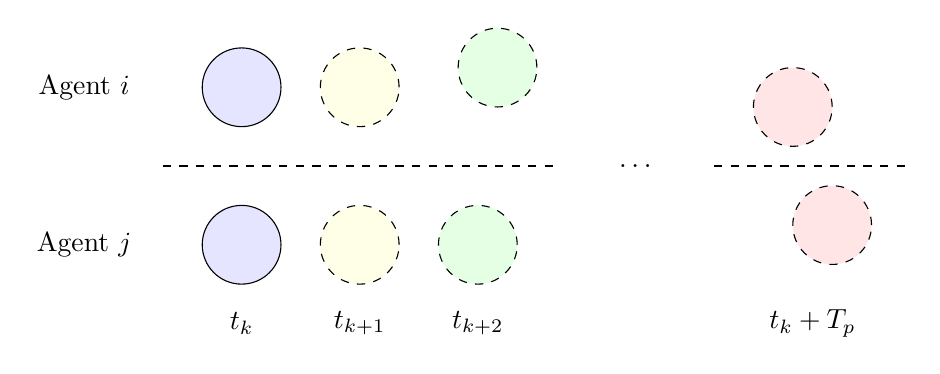
\begin{tikzpicture}[scale = 0.5]

  \draw[dashed] (0,0) -- (10,0);

  \node at (-2, 2) {Agent $i$};
  \node at (-2, -2) {Agent $j$};

  \filldraw[fill=blue!10!white, draw=black](2,2) circle (1cm);
  \filldraw[fill=blue!10!white, draw=black](2,-2) circle (1cm);
  \node at (2, -4) {$t_k$};


  \filldraw[fill=yellow!10!white, draw=black,dashed] (5,2) circle (1cm);
  \filldraw[fill=yellow!10!white, draw=black,dashed] (5,-2) circle (1cm);
  \node at (5, -4) {$t_{k+1}$};

  \filldraw[fill=green!10!white, draw=black,dashed] (8.5, 2.5) circle (1cm);
  \filldraw[fill=green!10!white, draw=black,dashed] (8,-2) circle (1cm);
  \node at (8, -4) {$t_{k+2}$};

  \node at (12, 0) {$\dots$};

  \draw[dashed] (14,0) -- (19,0);

  \filldraw[fill=red!10!white, draw=black,dashed] (16, 1.5) circle (1cm);
  \filldraw[fill=red!10!white, draw=black,dashed] (17,-1.5) circle (1cm);
  \node at (16.5, -4) {$t_k + T_p$};

\end{tikzpicture}

  \caption{The inter-agent constraint regime for two agents, $i,j$. Fully
    outlined circles denote measured configurations, while partly outlined
    circles denote predicted configurations. During the solution to the
    individual optimization problems, the predicted configuration of each agent
    at each timestep is constrained by the predicted configuration of the other
    agent at the same timestep (hence the homologously identical colours at
    each discrete timestep).}
  \label{fig:constraint_regime_horizon}
\end{figure}


The functions
$F_i : \mathcal{E}_{i,s} \times \mathcal{U}_i \to \mathbb{R}_{\geq 0}$ and
$V_i: \Omega_i \to \mathbb{R}_{\geq 0}$ are defined as
\begin{align}
  F_i \big(\overline{\vect{e}}_i(t), \overline{\vect{u}}_i(t)\big)
    &\triangleq \overline{\vect{e}}_i(t)^{\top} \mat{Q}_i \overline{\vect{e}}_i(t)
  + \overline{\vect{u}}_i(t)^{\top} \mat{R}_i \overline{\vect{u}}_i(t) \label{eq:F_i_def} \\[2.5ex]
  V_i \big(\overline{\vect{e}}_i(t)\big) & \triangleq \overline{\vect{e}}_i(t)^{\top} \mat{P}_i \overline{\vect{e}}_i(t) \label{eq:V_i_def}
\end{align}
Matrices $\mat{R}_i \in \mathbb{R}^{6 \times 6}$ and
$\mat{Q}_i, \mat{P}_i \in \mathbb{R}^{12 \times 12}$ are symmetric and positive
definite.  The running costs $F_i$ are upper- and lower-bounded by class
$\mathcal{K}_{\infty}$ functions:

\begin{bw_box}
  \begin{lemma} (\textit{$F_i$ is lower- and upper-bounded by class $\mathcal{K}_{\infty}$ functions})
    \label{lemma:F_i_bounded_K_class}

    Let functions $\alpha_1, \alpha_2 \in \mathcal{K}_{\infty}$ and $F_i$
    be defined by \eqref{eq:F_i_def}. Then, for all
    $\vect{e}_i \in \mathcal{E}_{i,s}$
    \begin{align}
      \alpha_1\big(\|\vect{e}_i\|\big) \leq F_i\big(\vect{e}_i, \vect{u}_i\big) \leq \alpha_2\big(\| \vect{e}_i \|\big)
    \end{align}
  \end{lemma}
\end{bw_box}


\begin{bw_box}
  \begin{lemma} ($F_i$ is Lipschitz continuous in $\mathcal{E}_{i,s} \times \mathcal{U}_i$)
\label{lemma:F_Lipschitz}

  Suppose that $\vect{e}_1, \vect{e}_2 \in \mathcal{E}_{i,s}$,
  $\vect{u}_i \in \mathcal{U}_i$ and that $F_i$ is defined by \eqref{eq:F_i_def}.
  The running costs $F_i$ are Lipschitz continuous in
  $\mathcal{E}_{i,s} \times \mathcal{U}_i$:
  $$\big|F_i(\vect{e}_1, \vect{u}_i) - F_i(\vect{e}_2, \vect{u}_i)\big| \leq L_{F_i} \|\vect{e}_1 - \vect{e}_2\|$$
  with Lipschitz constant $L_{F_i} = 2 \sigma_{max}(\mat{Q}_i) \overline{\varepsilon}_i $,
  where $\overline{\varepsilon}_i = \text{sup}\limits_{\vect{e}_i \in \mathcal{E}_{i,s}} \|\vect{e}_i\|$

\end{lemma}
\end{bw_box}


The terminal set $\Omega_i \subseteq \mathcal{E}_{i,t_k + T_p}$ is an admissible
positively invariant set according to definition
\eqref{def:positively_invariant} for system
\eqref{eq:position_based_error_model} such that
\begin{align}
  \Omega_i = \{\vect{e}_i \in \mathcal{E}_{i,t_k + T_p} : V_i(\vect{e}_i) \leq \varepsilon_{\Omega_i} \}
\end{align}
where $\varepsilon_{\Omega_i}$ is an arbitrarily small but fixed positive real scalar.

With regard to the terminal penalty function $V_i$, the following lemma will
prove to be useful in guaranteeing the convergence of the solution to the
optimal control problem to the terminal region $\Omega_i$:

\begin{bw_box}
\begin{lemma} ($V_i$ is Lipschitz continuous in $\Omega_i$)
\label{lemma:V_Lipschitz_e_0}

  Suppose that $\vect{e}_1, \vect{e}_2 \in \Omega_i$, and that
  $V_i$ is defined by \eqref{eq:V_i_def}. The terminal penalty function
  $V_i$ is Lipschitz continuous in $\Omega_i$
  $$\big|V_i(\vect{e}_1) - V_i(\vect{e}_2)\big| \leq L_{V_i} \|\vect{e}_1 - \vect{e}_2\|$$
  with Lipschitz constant $L_{V_i} = 2 \sigma_{max}(\mat{P}_i) \overline{\varepsilon}_{i,\Omega_i} $\\

  where $\overline{\varepsilon}_{i,\Omega_i} = \text{sup}\limits_{\vect{e}_i \in \Omega_i} \|\vect{e}_i\|$


\end{lemma}
\end{bw_box}


Furthermore, $V_i$ is lower- and upper-bounded by class $\mathcal{K}_{\infty}$ functions.

\begin{bw_box}
  \begin{lemma} (\textit{$V_i$ is lower- and upper-bounded by class
      \label{lemma:V_i_lower_upper_bounded}
    $\mathcal{K}_{\infty}$ functions in $\Omega_i$})
  \end{lemma}

  Let $\alpha_1, \alpha_2 \in \mathcal{K}_{\infty}$, $\vect{e}_i \in \Omega_i$
  and let $V_i$ be defined by \eqref{eq:V_i_def}. Then
  \begin{align}
    \alpha_1\big(\|\vect{e}_i\|\big) \leq V_i(\vect{e}_i) \leq \alpha_2\big(\| \vect{e}_i \|\big)
  \end{align}

\end{bw_box}


The solution to the optimal control problem \eqref{position_based_cost}
at time $t_k$ is an optimal control input, denoted by
$\overline{\vect{u}}_i^{\star}(\cdot;\ \vect{e}_i(t_k))$, which
is applied to the open-loop system until the next sampling instant $t_k + h$,
with $h \in (0,T_p)$:
\begin{align}
  %\vect{u}_i\big(t;\ \vect{e}_i(t_k)\big) = \overline{\vect{u}}_i^{\star}\big(t;\ \vect{e}_i(t_k)\big),\  t \in [t_k, t_k + h) \nonumber \\[2.5ex]
  \vect{u}_i(t) = \overline{\vect{u}}_i^{\star}\big(t;\ \vect{e}_i(t_k)\big),\  t \in [t_k, t_k + h]
 \label{eq:position_based_optimal_u}
\end{align}
At time $t_{k+1}$ a new finite horizon optimal control problem is solved in the
same manner, leading to a receding horizon approach.

The control input $\vect{u}_i(\cdot)$ is of feedback form,
since it is recalculated at each sampling instant based on the then-current
state. The solution to equation \eqref{eq:position_based_error_model} $-$ the
model of the real system, starting at time $t_1$, from an initial condition
$\vect{e}_i(t_1) = \overline{\vect{e}}_i(t_1)$,
by application of the control input $\vect{u}_i : [t_1, t_2] \to \mathcal{U}_i$
is denoted by
\begin{align}
  \vect{e}_i\big(t;\ \vect{u}_i(\cdot), \vect{e}_i(t_1)\big),\ t \in [t_1, t_2]
\end{align}


On the existence of solutions to \eqref{eq:position_based_error_model} we
assume the following:
\begin{bw_box}
\begin{assumption}
  \label{ass:existence_of_solutions_without_disturbance}

  The system \eqref{eq:position_based_error_model} has a
  \textit{continuous solution} for any $\vect{e}_i(0) \in \mathcal{E}_{i,0}$ and
  any \textit{piecewise continuous} input
  $\vect{u}_i(\cdot) :[0,T_p] \to \mathcal{U}_i$.
\end{assumption}
\end{bw_box}

The states of the open-loop system \eqref{eq:internal_error_model} $-$ the
predicted states obey the following notation:
\begin{bw_box}
\begin{remark}
The \textit{predicted} state of the system \eqref{eq:position_based_error_model}
at time $\tau \geq t_k$ , based on the measurement of the state at time
$t_k$, $\vect{e}_i(t_k)$, by application of the control input
\eqref{eq:position_based_optimal_u}, is denoted by
\begin{align}
  \overline{\vect{e}}_i\big(\tau;\ \vect{u}_i(\tau), \vect{e}_i(t_k)\big) \label{eq:position_based_predicted_error_0}
\end{align}
\end{remark}
\end{bw_box}

The closed-loop system for which stability is to be guaranteed is
\begin{align}
  \vect{e}_i(\tau) = g_i\big(\vect{e}_i(\tau), \overline{\vect{u}}_i^{\star}(\tau)\big),\ \tau \geq t_0 = 0
  \label{eq:without_disturbances_closed_loop}
\end{align}
where $\overline{\vect{u}}_i^{\star}(\tau) = \overline{\vect{u}}_i^{\star}(\tau;\ \vect{e}_i(t_k))$,
$\tau \in [t_k, t_k + h)$ and $t_0 = 0$.


We can now give the definition of an \textit{admissible input} for the FHOCP
\eqref{problem:opt_without_disturbances}:

\begin{bw_box}
  \begin{definition} (\textit{Admissible input for the FHOCP
\eqref{problem:opt_without_disturbances}})
  \label{definition:admissible_input}

  A control input $\vect{u}_i : [t_k, t_k + T_p] \to \mathbb{R}^6$ for a state
  $\vect{e}_i(t_k)$ is called \textit{admissible} for the problem
  \eqref{problem:opt_without_disturbances} if all the following hold:

  \begin{enumerate}
    \item $\vect{u}_i(\cdot)$ is piecewise continuous
    \item $\vect{u}_i(\tau) \in \mathcal{U}_i,\ \forall \tau \in [t_k, t_k + T_p]$
    \item $\overline{\vect{e}}_i\big(\tau;\ \vect{u}_i(\cdot), \vect{e}_i(t_k)\big) \in \mathcal{E}_{i,\tau},\ \forall \tau \in [t_k, t_k + T_p]$
    \item $\overline{\vect{e}}_i\big(t_k + T_p;\ \vect{u}_i(\cdot), \vect{e}_i(t_k)\big) \in \Omega_i$
  \end{enumerate}

  In other words, $\vect{u}_i$ is admissible if it conforms to the constraints
  on the input and its application yields states that conform to the
  prescribed state constraints of problem
  \eqref{problem:opt_without_disturbances} along the entire horizon
  $[t_k, t_k + T_p]$, and the terminal predicted state conforms to the
  terminal constraint.

\end{definition}
\end{bw_box}

    %-------------------------------------------------------------------------------
\section{Stabilization: Feasibility and Convergence}

Under these considerations, we can now state the theorem that relates to
the guaranteeing of the stability of the compound system of agents
$i \in \mathcal{V}$, when each of them is assigned a desired
position which results in feasible displacements:\\[2.5ex]

\begin{bw_box}
\begin{theorem}

  Suppose that

  \begin{enumerate}
    \item the terminal region $\Omega_i \subseteq \mathcal{E}_{i,s}$ is
      closed with $\vect{0} \in \Omega_i$
    \item a solution to the optimal control problem \eqref{position_based_cost}
      is feasible at time $t=0$, that is, assumptions
      \eqref{ass:measurements_access}, \eqref{ass:initial_conditions}, and
      \eqref{ass:intra_environmental_arrangement} hold at time $t=0$
    \item assumptions \eqref{ass:g_i_Lipschitz}, \eqref{ass:access_to_predicted_info_n},
      and \eqref{ass:existence_of_solutions_without_disturbance} hold
    \item there exists an admissible control input
      $h_i(\vect{e}_i) : [t_k + T_p, t_{k+1} + T_p] \to \mathcal{U}_i$
      such that for all $\vect{e}_i \in \Omega_i$ and
      $\forall \tau \in [t_k + T_p, t_{k+1} + T_p]$:

      \begin{enumerate}
        \item $\vect{e}_i(\tau) \in \Omega_i$
        \item $\dfrac{\partial V_i}{\partial \vect{e}_i} g_i\big(\vect{e}_i(\tau),
        h_i\big(\vect{e}_i(\tau)\big)
          + F_i\big(\vect{e}_i(\tau), h_i\big(\vect{e}_i(\tau)\big)\big) \leq 0$
      \end{enumerate}

  \end{enumerate}

  then the closed loop system \eqref{eq:without_disturbances_closed_loop} under
  the control input \eqref{eq:position_based_optimal_u} converges to the set
  $\Omega_i$ when $t \to \infty$.

\end{theorem}
\end{bw_box}

\textbf{Proof}. The proof of the above theorem consists of two parts:
in the first, recursive feasibility is established, that is, initial
feasibility is shown to imply subsequent feasibility; in the second, and based
on the first part, it is shown that the error state $\vect{e}_i(t)$ converges
to the terminal set $\Omega_i$.\\[2.5ex]

\textbf{Feasibility analysis}
Consider a sampling instant $t_k$ for which a
solution $\overline{\vect{u}}_i^{\star}\big(\cdot;\ \vect{e}_i(t_k)\big)$ to
\eqref{position_based_cost} exists.
%In between $t_k$ and $t_k + h$,
%where $h$ is the sampling time, the optimal control signal
%$\vect{u}_i^{\star}\big(\cdot;\ \vect{e}_i(t_k)\big)$ is applied to the open-loop
%system.
Suppose now a time instant $t_{k+1}$ such that\footnote{It is not strictly necessary
that $t_{k+1} = t_k + h$ here, however it is necessary for the following that
$t_{k+1} - t_k \leq h$} $t_k < t_{k+1} < t_k + T_p$, and consider that the
optimal control signal calculated at $t_k$ is comprised by the following two
portions:

\begin{equation}
  \overline{\vect{u}}_i^{\star}\big(\cdot;\ \vect{e}_i(t_k)\big) = \left\{
      \begin{array}{ll}
        \overline{\vect{u}}_i^{\star}\big(\tau_1;\ \vect{e}_i(t_k)\big), & \tau_1 \in [t_k, t_{k+1}] \\[2.5ex]
        \overline{\vect{u}}_i^{\star}\big(\tau_2;\ \vect{e}_i(t_k)\big), & \tau_2 \in [t_{k+1}, t_k + T_p]
      \end{array}
      \right.
  \label{eq:optimal_input_portions_without_disturbances}
\end{equation}

Both portions are admissible since the calculated optimal control input is
admissible, and hence they both conform to the input constraints.
As for the resulting predicted states, they satisfy the state constraints, and,
crucially: $\overline{\vect{e}}_i\big(t_k + T_p;\ \overline{\vect{u}}_i^{\star}(\cdot), \vect{e}_i(t_k)\big) \in \Omega_i$.
Furthermore, according to assumption (3) of the theorem, there exists an
admissible (and certainly not guaranteed optimal) input $h_i(\vect{e}_i)$ that
renders $\Omega_i$ invariant over $[t_k + T_p, t_{k+1} + T_p]$.

Given the above facts, we can construct an admissible input
$\widetilde{\vect{u}}_i(\cdot)$  starting at time $t_{k+1}$ by sewing together
the second portion of \eqref{eq:optimal_input_portions_without_disturbances}
and the input $h_i(\vect{e}_i)$:

\begin{equation}
  \widetilde{\vect{u}}_i(\tau) = \left\{
      \begin{array}{ll}
        \overline{\vect{u}}_i^{\star}\big(\tau;\ \vect{e}_i(t_k)\big), & \tau \in [t_{k+1}, t_k + T_p] \\[2.5ex]
        h_i\big(\vect{e}_i(\tau)\big), & \tau \in (t_k + T_p, t_{k+1} + T_p]
      \end{array}
      \right.
\label{eq:optimal_input_t_plus_one_without_disturbances}
\end{equation}

The control input $\widetilde{\vect{u}}_i(\cdot)$ is admissible as a
composition of admissible control inputs. This means that feasibility of a
solution to the optimization problem at time $t_k$ implies feasibility at
time $t_{k+1} > t_k$, and, thus, since at time $t=0$ a solution is assumed to
be feasible, a solution to the optimal control problem is feasible for all
$t \geq 0$.\\[2.5ex]

\textbf{Convergence analysis}
The second part of the proof involves demonstrating the convergence of the
state $\vect{e}_i$ to the terminal set $\Omega_i$. In order for this
to be proved, it must be shown that a proper value function decreases along
closed-loop trajectories starting at some initial time $t_k$. We consider the
\textit{optimal} cost $J_i^{\star}\big(\vect{e}_i(t)\big)$ as a candidate
Lyapunov function:
$$J_i^{\star}\big(\vect{e}_i(t)\big) \triangleq J_i \Big(\vect{e}_i(t), \overline{\vect{u}}_i^{\star}\big(\cdot;\ \vect{e}_i(t)\big)\Big)$$
and, in particular, our goal is to show that that this cost decreases over
consecutive sampling instants $t_{k+1} = t_k + h$, i.e.
$J_i^{\star}\big(\vect{e}_i(t_{k+1})\big) - J_i^{\star}\big(\vect{e}_i(t_k)\big) \leq 0$.\\[2.5ex]

In order not to wreak notational havoc, let us define the following terms:
\begin{gg_box}
\begin{itemize}
  \item $\vect{u}_{0,i}(\tau) \triangleq \overline{\vect{u}}_i^{\star}\big(\tau;\ \vect{e}_i(t_k)\big)$
    as the \textit{optimal} input that results from the solution to problem
    \eqref{problem:opt_without_disturbances} based on the measurement of state
    $\vect{e}_i(t_k)$, applied at time $\tau \geq t_k$
  \item $\vect{e}_{0,i}(\tau) \triangleq \overline{\vect{e}}_i\big(\tau;\ \overline{\vect{u}}_i^{\star}\big(\cdot;\ \vect{e}_i(t_k)\big), \vect{e}_i(t_k)\big)$
    as the \textit{predicted} state at time $\tau \geq t_k$, that is,
    the state that results from the application of the above input
    $\overline{\vect{u}}_i^{\star}\big(\cdot;\ \vect{e}_i(t_k)\big)$ to the
    state $\vect{e}_i(t_k)$, at time $\tau$
  \item $\vect{u}_{1,i}(\tau) \triangleq \widetilde{\vect{u}}_i(\tau)$
    as the \textit{admissible} input at $\tau \geq t_{k+1}$
    (see eq. \eqref{eq:optimal_input_t_plus_one_without_disturbances})
  \item $\vect{e}_{1,i}(\tau) \triangleq \overline{\vect{e}}_i\big(\tau;\ \widetilde{\vect{u}}_i(\cdot), \vect{e}_i(t_{k+1})\big)$
    as the \textit{predicted} state at time $\tau \geq t_{k+1}$, that is,
    the state that results from the application of the above input
    $\widetilde{\vect{u}}_i(\cdot)$ to the state
    $\vect{e}_i\big(t_{k+1};\ \overline{\vect{u}}_i^{\star}\big(\cdot;\ \vect{e}_i(t_k)\big), \vect{e}_i(t_k)\big)$, at time $\tau$
\end{itemize}
\end{gg_box}

\begin{bw_box}
  \begin{remark}
  \label{remark:predicted_actual_equations_without_disturbance}
    Given that no model mismatch or disturbances exist, for
    the predicted and actual states at time
    $\tau_1 \geq \tau_0 \in \mathbb{R}_{\geq 0}$ it holds that:
    \begin{align}
      \vect{e}_i\big(\tau_1;\ \vect{u}_i(\cdot), \vect{e}_i(\tau_0)\big) &=
        \vect{e}_i(\tau_0) + \int_{\tau_0}^{\tau_1} g_i\big(\vect{e}_i(s;\ \vect{e}_i(\tau_0)), \vect{u}_i(s)\big) ds \\[2.5ex]
      \overline{\vect{e}}_i\big(\tau_1;\ \vect{u}_i(\cdot), \vect{e}_i(\tau_0)\big) &=
        \vect{e}_i(\tau_0) + \int_{\tau_0}^{\tau_1} g_i\big(\overline{\vect{e}}_i(s;\ \vect{e}_i(\tau_0)), \vect{u}_i(s)\big) ds
    \end{align}
  \end{remark}
\end{bw_box}

Before beginning to prove convergence, it is worth noting that while the cost
$$J_i \Big(\vect{e}_i(t), \overline{\vect{u}}_i^{\star}\big(\cdot;\ \vect{e}_i(t)\big)\Big)$$
is optimal (in the sense that it is based on the optimal input, which provides
its minimum realization), a cost that is based on a plainly admissible
(and thus, without loss of generality, sub-optimal) input
$\vect{u}_i \not= \overline{\vect{u}}_i^{\star}$ will result in a configuration where
\begin{equation}
J_i \Big(\vect{e}_i(t), \vect{u}_i\big(\cdot;\ \vect{e}_i(t)\big)\Big)
\geq J_i \Big(\vect{e}_i(t), \overline{\vect{u}}_i^{\star}\big(\cdot;\ \vect{e}_i(t)\big)\Big)
\end{equation}

Let us now begin our investigation on the difference between the cost
that results from the application of the feasible input $\vect{u}_{1,i}$,
which we shall denote by $\overline{J}_i\big(\vect{e}_i(t_{k+1})\big)$,
and the optimal cost $J_i^{\star}\big(\vect{e}_i(t_k)\big)$. We remind
ourselves that
$J_i \big(\vect{e}_i(t), \overline{\vect{u}}_i (\cdot)\big)$ $=$
$\int_{t}^{t + T_p} F_i \big(\overline{\vect{e}}_i(s), \overline{\vect{u}}_i (s)\big) ds$ $+$
$V_i \big(\overline{\vect{e}}_i (t + T_p)\big)$:
\begin{align}
  \overline{J}_i\big(\vect{e}_i(t_{k+1})\big) - J_i^{\star}\big(\vect{e}_i(t_k)\big) =\
   & V_i \big(\vect{e}_{1,i} (t_{k+1} + T_p)\big) + \int_{t_{k+1}}^{t_{k+1} + T_p} F_i \big(\vect{e}_{1,i}(s), \vect{u}_{1,i} (s)\big) ds \\[2.5ex]
  -&V_i \big(\vect{e}_{0,i} (t_k + T_p)\big) - \int_{t_k}^{t_k + T_p} F_i \big(\vect{e}_{0,i}(s), \vect{u}_{0,i} (s)\big) ds
\end{align}
Considering that $t_k < t_{k+1} < t_k + T_p < t_{k+1} + T_p$, we break down the
two integrals above in between these intervals:
\begin{align}
  \overline{J}_i\big(\vect{e}_i(t_{k+1})\big) - J_i^{\star}\big(\vect{e}_i(t_k)\big) &= \\[2.5ex]
    V_i \big(\vect{e}_{1,i} (t_{k+1} + T_p)\big)
    &+ \int_{t_{k+1}}^{t_k + T_p} F_i \big(\vect{e}_{1,i}(s), \vect{u}_{1,i} (s)\big) d s
    + \int_{t_k + T_p}^{t_{k+1} + T_p} F_i \big(\vect{e}_{1,i}(s), \vect{u}_{1,i} (s)\big) d s \\[2.5ex]
    -V_i \big(\vect{e}_{0,i} (t_k + T_p)\big)
    &- \int_{t_k}^{t_{k+1}} F_i \big(\vect{e}_{0,i}(s), \vect{u}_{0,i} (s)\big) d s
    - \int_{t_{k+1}}^{t_k + T_p} F_i \big(\vect{e}_{0,i}(s), \vect{u}_{0,i} (s)\big) d s
\label{eq:convergence_4_integrals}
\end{align}

\begin{gg_box}

Since no model mismatch or disturbances are present, consulting with remark
\eqref{remark:predicted_actual_equations_without_disturbance} and substituting
for $\tau_0 = t_k$ and $\tau_1 = t_{k+1}$ yields:
\begin{align}
  \vect{e}_i\big(t_{k+1};\ \overline{\vect{u}}_i^{\star}\big(\cdot;\ \vect{e}_i(t_k)\big), \vect{e}_i(t_k)\big) &=
    \vect{e}_i(t_k) + \int_{t_k}^{t_{k+1}} g_i\big(\vect{e}_i(s;\ \vect{e}_i(t_k)), \overline{\vect{u}}_i^{\star}(s)\big) ds \\[2.5ex]
  \overline{\vect{e}}_i\big(t_{k+1};\ \overline{\vect{u}}_i^{\star}\big(\cdot;\ \vect{e}_i(t_k)\big), \vect{e}_i(t_k)\big) &=
    \vect{e}_i(t_k) + \int_{t_k}^{t_{k+1}} g_i\big(\overline{\vect{e}}_i(s;\ \vect{e}_i(t_k)), \overline{\vect{u}}_i^{\star}(s)\big) ds
\end{align}
Subtracting the second expression from the first, we get
\begin{align}
  \vect{e}_i\big(t_{k+1};\ &\overline{\vect{u}}_i^{\star}\big(\cdot;\ \vect{e}_i(t_k)\big), \vect{e}_i(t_k)\big) -
  \overline{\vect{e}}_i\big(t_{k+1};\ \overline{\vect{u}}_i^{\star}\big(\cdot;\ \vect{e}_i(t_k)\big), \vect{e}_i(t_k)\big) \\[2.5ex]
  &=\int_{t_k}^{t_{k+1}} g_i\big(\vect{e}_i(s;\ \vect{e}_i(t_k)), \overline{\vect{u}}_i^{\star}(s)\big) ds -
    \int_{t_k}^{t_{k+1}} g_i\big(\overline{\vect{e}}_i(s;\ \vect{e}_i(t_k)), \overline{\vect{u}}_i^{\star}(s)\big) ds\\[2.5ex]
  &=\int_{t_k}^{t_{k+1}} \bigg( g_i\big(\vect{e}_i(s;\ \vect{e}_i(t_k)), \overline{\vect{u}}_i^{\star}(s)\big)
  - g_i\big(\overline{\vect{e}}_i(s;\ \vect{e}_i(t_k)), \overline{\vect{u}}_i^{\star}(s)\big) \bigg) ds \\[2.5ex]
\end{align}
Taking norms on either side yields
\begin{align}
  \bigg\|\vect{e}_i\big(t_{k+1};\ &\overline{\vect{u}}_i^{\star}\big(\cdot;\ \vect{e}_i(t_k)\big), \vect{e}_i(t_k)\big)
    -\overline{\vect{e}}_i\big(t_{k+1};\ \overline{\vect{u}}_i^{\star}\big(\cdot;\ \vect{e}_i(t_k)\big), \vect{e}_i(t_k)\big) \bigg\| \\[2.5ex]
  &=\bigg\|\int_{t_k}^{t_{k+1}} \bigg( g_i\big(\vect{e}_i(s;\ \vect{e}_i(t_k)), \overline{\vect{u}}_i^{\star}(s)\big)
  - g_i\big(\overline{\vect{e}}_i(s;\ \vect{e}_i(t_k)), \overline{\vect{u}}_i^{\star}(s)\big) \bigg) ds \bigg\|\\[2.5ex]
  &=\int_{t_k}^{t_{k+1}} \bigg\| g_i\big(\vect{e}_i(s;\ \vect{e}_i(t_k)), \overline{\vect{u}}_i^{\star}(s)\big)
  - g_i\big(\overline{\vect{e}}_i(s;\ \vect{e}_i(t_k)), \overline{\vect{u}}_i^{\star}(s)\big) \bigg\| ds\\[2.5ex]
  &\leq L_{g_i}\int_{t_k}^{t_{k+1}} \bigg\|
    \vect{e}_i\big(s;\ \overline{\vect{u}}_i^{\star}\big(\cdot;\ \vect{e}_i(t_k)\big), \vect{e}_i(t_k)\big)
    -\overline{\vect{e}}_i\big(s;\ \overline{\vect{u}}_i^{\star}\big(\cdot;\ \vect{e}_i(t_k)\big), \vect{e}_i(t_k)\big) \bigg\| ds
\end{align}
since $g_i$ is Lipschitz continuous in $\mathcal{E}_{i,s}$ with Lipschitz constant
$L_{g_i}$. Reformulation yields
\begin{align}
  \bigg\|\vect{e}_i\big(t_k&+h;\ \overline{\vect{u}}_i^{\star}\big(\cdot;\ \vect{e}_i(t_k)\big), \vect{e}_i(t_k)\big)
    -\overline{\vect{e}}_i\big(t_k+h;\ \overline{\vect{u}}_i^{\star}\big(\cdot;\ \vect{e}_i(t_k)\big), \vect{e}_i(t_k)\big) \bigg\| \\[2.5ex]
  &\leq L_{g_i}\int_{0}^{h} \bigg\|
    \vect{e}_i\big(t_k + s;\ \overline{\vect{u}}_i^{\star}\big(\cdot;\ \vect{e}_i(t_k)\big), \vect{e}_i(t_k)\big)
    -\overline{\vect{e}}_i\big(t_k + s;\ \overline{\vect{u}}_i^{\star}\big(\cdot;\ \vect{e}_i(t_k)\big), \vect{e}_i(t_k)\big) \bigg\| ds
\end{align}
By applying the Gr\"{o}nwall-Bellman inequality we obtain zero as an
upper bound for the norm of the difference between the two states. Since
any norm cannot be negative, we conclude that
\begin{align}
  \bigg\|\vect{e}_i\big(t_{k+1};\ \overline{\vect{u}}_i^{\star}\big(\cdot;\ \vect{e}_i(t_k)\big), \vect{e}_i(t_k)\big)
    -\overline{\vect{e}}_i\big(t_{k+1};\ \overline{\vect{u}}_i^{\star}\big(\cdot;\ \vect{e}_i(t_k)\big), \vect{e}_i(t_k)\big) \bigg\| = 0
\end{align}
which means that
\begin{align}
  \vect{e}_i\big(t_{k+1};\ \overline{\vect{u}}_i^{\star}\big(\cdot;\ \vect{e}_i(t_k)\big), \vect{e}_i(t_k)\big)
    =\overline{\vect{e}}_i\big(t_{k+1};\ \overline{\vect{u}}_i^{\star}\big(\cdot;\ \vect{e}_i(t_k)\big), \vect{e}_i(t_k)\big)
\end{align}

In between times $t_{k+1}$ and $t_k + T_p$, the constructed admissible input
$\widetilde{\vect{u}}_i(\cdot)$ is equal to the optimal
input $\overline{\vect{u}}_i^{\star}\big(\cdot;\ \vect{e}_i(t_k)\big)$
(see eq. \ref{eq:optimal_input_t_plus_one_without_disturbances}), which means
that $\vect{u}_{1,i}(\tau) = \vect{u}_{0,i}(\tau)$ in the interval
$\tau \in [t_{k+1}, t_k + T_p]$. Since the initial conditions at $t=t_{k+1}$ are
equal and the control laws are also equal, so will the predicted states over the
same interval:
\begin{align}
  \overline{\vect{e}}_i\big(\tau;\ \widetilde{\vect{u}}_i(\cdot), \vect{e}_i(t_{k+1})\big) =
  \overline{\vect{e}}_i\big(\tau;\ \overline{\vect{u}}_i^{\star}(\cdot), \overline{\vect{e}}_i(t_{k+1})\big), \ \tau \in [t_{k+1}, t_k + T_p]
  \label{eq:equal_predicted_without_disturbance}
\end{align}
Using our notation then, in the same interval:
$\vect{e}_{1,i}(\cdot) = \vect{e}_{0,i}(\cdot)$. Coupled with the fact that
in the same interval $\vect{u}_{1,i}(\tau) = \vect{u}_{0,i}(\tau)$, the following
equality holds over $[t_{k+1}, t_k + T_p]$:
\begin{align}
  F_i \big(\vect{e}_{1,i}(s), \vect{u}_{1,i} (s)\big) =
  F_i \big(\vect{e}_{0,i}(s), \vect{u}_{0,i} (s)\big),\ s \in [t_{k+1}, t_k + T_p]
\end{align}
Integrating this equality over the interval where it is valid yields
\begin{align}
  \int_{t_{k+1}}^{t_k + T_p}F_i \big(\vect{e}_{1,i}(s), \vect{u}_{1,i} (s)\big) ds =
  \int_{t_{k+1}}^{t_k + T_p}F_i \big(\vect{e}_{0,i}(s), \vect{u}_{0,i} (s)\big) ds
\end{align}
\end{gg_box}
This means that these two integrals with ends over the interval
$[t_{k+1}, t_k + T_p]$ featured in the right-hand side of eq.
\eqref{eq:convergence_4_integrals} vanish, and thus the cost difference becomes
\begin{align}
  \overline{J}_i\big(\vect{e}_i(t_{k+1})\big) - J_i^{\star}\big(\vect{e}_i(t_k)\big) &=
    V_i \big(\vect{e}_{1,i} (t_{k+1} + T_p)\big)
    +\int_{t_k + T_p}^{t_{k+1} + T_p} F_i \big(\vect{e}_{1,i}(s), \vect{u}_{1,i} (s)\big) d s \\[2.5ex]
    &-V_i \big(\vect{e}_{0,i} (t_k + T_p)\big)
    -\int_{t_k}^{t_{k+1}} F_i \big(\vect{e}_{0,i}(s), \vect{u}_{0,i} (s)\big) d s
\label{eq:convergence_2_integrals}
\end{align}

During the course of arriving at the above result, we have concluded that,
in the absence of disturbances, the remark \eqref{eq:error_now_to_predicted_error}
holds.
\begin{bw_box}
  \begin{remark}
  \label{eq:error_now_to_predicted_error}
    In the absence of disturbances, the following equality holds over
    the entire horizon $t \in [t_k, t_k + T_p]$:
    \begin{align}
      \vect{e}_i\big(t;\ \overline{\vect{u}}_i^{\star}\big(\cdot;\ \vect{e}_i(t_k)\big), \vect{e}_i(t_k)\big)
        =\overline{\vect{e}}_i\big(t;\ \overline{\vect{u}}_i^{\star}\big(\cdot;\ \vect{e}_i(t_k)\big), \vect{e}_i(t_k)\big)
    \end{align}
  \end{remark}
\end{bw_box}

\begin{gg_box}
  We turn our attention to the first integral in the above expression, and we
  note that $[t_{k+1} + T_p, t_k + T_p]$, is exactly the
  the interval where assumption (3b) of the theorem holds. Hence,
  we decide to integrate the expression found in the assumption over the
  interval $[t_k + T_p, t_{k+1} + T_p]$, for the controls and states applicable
  in it:
  \begin{align}
    \int_{t_k + T_p}^{t_{k+1} + T_p} \Bigg(\dfrac{\partial V_i}{\partial \vect{e}_{1,i}} g_i\big(\vect{e}_{1,i}(s), \vect{u}_{1,i}(s)\big)
    + F_i\big(\vect{e}_{1,i}(s), \vect{u}_{1,i}(s)\big)\Bigg) ds &\leq 0 \\[2.5ex]
    \int_{t_k + T_p}^{t_{k+1} + T_p} \dfrac{d}{ds} V_i\big(\vect{e}_{1,i}(s)\big) d s
    + \int_{t_k + T_p}^{t_{k+1} + T_p} F_i\big(\vect{e}_{1,i}(s), \vect{u}_{1,i}(s)\big) ds &\leq 0 \\[2.5ex]
    V_i\big(\vect{e}_{1,i}(t_{k+1} + T_p)\big) - V_i\big(\vect{e}_{1,i}(t_k + T_p)\big)
    + \int_{t_k + T_p}^{t_{k+1} + T_p} F_i\big(\vect{e}_{1,i}(s), \vect{u}_{1,i}(s)\big) ds &\leq 0 \\[2.5ex]
    V_i\big(\vect{e}_{1,i}(t_{k+1} + T_p)\big)
    + \int_{t_k + T_p}^{t_{k+1} + T_p} F_i\big(\vect{e}_{1,i}(s), \vect{u}_{1,i}(s)\big) ds &\leq V_i\big(\vect{e}_{1,i}(t_k + T_p)\big)
  \end{align}

  The left-hand side expression is the same as the first two terms in the
  right-hand side of equality \eqref{eq:convergence_2_integrals}. We can
  introduce the third one by subtracting it from both sides:
  \begin{align}
    V_i\big(\vect{e}_{1,i}(t_{k+1} + T_p)\big)
    &+ \int_{t_k + T_p}^{t_{k+1} + T_p} F_i\big(\vect{e}_{1,i}(s), \vect{u}_{1,i}(s)\big) ds
    - V_i\big(\vect{e}_{0,i}(t_k + T_p)\big) \\[2.5ex]
    &\leq V_i\big(\vect{e}_{1,i}(t_k + T_p)\big)
    - V_i\big(\vect{e}_{0,i}(t_k + T_p)\big) \\[2.5ex]
    &\leq \Big|V_i\big(\vect{e}_{1,i}(t_k + T_p)\big)
    - V_i\big(\vect{e}_{0,i}(t_k + T_p)\big)\Big|
  \end{align}
  since $x \leq |x|, \forall x \in \mathbb{R}$.

  By revisiting lemma \eqref{lemma:V_Lipschitz_e_0}, the above inequality
  becomes
  \begin{align}
    V_i\big(\vect{e}_{1,i}(t_{k+1} + T_p)\big)
    + \int_{t_k + T_p}^{t_{k+1} + T_p} F_i\big(\vect{e}_{1,i}(s), \vect{u}_{1,i}(s)\big) ds
    - V_i\big(\vect{e}_{0,i}(t_k + T_p)\big) \\[2.5ex]
    \leq L_{V_i} \big\|\vect{e}_{1,i}(t_k + T_p) - \vect{e}_{0,i}(t_k + T_p)\big\|
  \end{align}

  However, as we witnessed in \eqref{eq:equal_predicted_without_disturbance},
  in the interval $[t_{k+1}, t_k + T_p]$:
  $\vect{e}_{1,i}(\cdot) = \vect{e}_{0,i}(\cdot)$, hence the right-hand
  side of the inequality equals zero:
  \begin{align}
    V_i\big(\vect{e}_{1,i}(t_{k+1} + T_p)\big)
    + \int_{t_k + T_p}^{t_{k+1} + T_p} F_i\big(\vect{e}_{1,i}(s), \vect{u}_{1,i}(s)\big) ds
    - V_i\big(\vect{e}_{0,i}(t_k + T_p)\big) \leq 0
  \end{align}

  By subtracting the fourth term needed to complete the right-hand side
  expression of \eqref{eq:convergence_2_integrals}, i.e.
  $\int_{t_k}^{t_{k+1}} F_i \big(\vect{e}_{0,i}(s), \vect{u}_{0,i} (s)\big) d s$
  from both sides we get
  \begin{align}
    V_i\big(\vect{e}_{1,i}(t_{k+1} + T_p)\big)
    + \int_{t_k + T_p}^{t_{k+1} + T_p} F_i\big(\vect{e}_{1,i}(s), \vect{u}_{1,i}(s)\big) ds& \\[2.5ex]
    - V_i\big(\vect{e}_{0,i}(t_k + T_p)\big)
    -\int_{t_k}^{t_{k+1}} F_i \big(\vect{e}_{0,i}(s), \vect{u}_{0,i} (s)\big) d s
    &\leq -\int_{t_k}^{t_{k+1}} F_i \big(\vect{e}_{0,i}(s), \vect{u}_{0,i} (s)\big) d s
  \end{align}

  The left-hand side of this inequality is now equal to the cost difference
  $\overline{J}_i\big(\vect{e}_i(t_{k+1})\big) - J_i^{\star}\big(\vect{e}_i(t_k)\big)$.
\end{gg_box}
Hence, the cost difference becomes bounded by
\begin{align}
  \overline{J}_i\big(\vect{e}_i(t_{k+1})\big) - J_i^{\star}\big(\vect{e}_i(t_k)\big) \leq
    -\int_{t_k}^{t_{k+1}} F_i \big(\vect{e}_{0,i}(s), \vect{u}_{0,i} (s)\big) ds
\end{align}
\begin{gg_box}
  $F_i$ is a positive-definite function as a sum of a positive-definite
  $\|\vect{u}_i\|^2_{\mat{R}_i}$ and a positive semi-definite function
  $\|\vect{e}_i\|^2_{\mat{Q}_i}$. If we denote by
  $m_i = \lambda_{min}(\mat{Q}_i, \mat{R}_i) \geq 0$ the minimum eigenvalue
  between those of matrices $\mat{R}_i, \mat{Q}_i$, this means that
  \begin{align}
    F_i \big(\vect{e}_{0,i}(s), \vect{u}_{0,i} (s)\big) \geq m_i \|\vect{e}_{0,i}(s)\|^2
  \end{align}

  By integrating the above between our interval of interest $[t_k, t_{k+1}]$ we get
  \begin{align}
    \int_{t_k}^{t_{k+1}} F_i \big(\vect{e}_{0,i}(s), \vect{u}_{0,i} (s)\big) &\geq \int_{t_k}^{t_{k+1}} m_i \|\vect{e}_{0,i}(s)\|^2 ds \\[2.5ex]
    \text{or}\\[2.5ex]
    -\int_{t_k}^{t_{k+1}} F_i \big(\vect{e}_{0,i}(s), \vect{u}_{0,i} (s)\big) &\leq -m_i \int_{t_k}^{t_{k+1}} \|\vect{e}_{0,i}(s)\|^2 ds
  \end{align}
\end{gg_box}

This means that the cost difference is upper-bounded by a class $\mathcal{K}$
function
\begin{align}
  \overline{J}_i\big(\vect{e}_i(t_{k+1})\big) - J_i^{\star}\big(\vect{e}_i(t_k)\big)
  &\leq -m_i \int_{t_k}^{t_{k+1}} \|\vect{e}_{0,i}(s)\|^2 ds \leq 0
\end{align}
and since the cost $\overline{J}_i\big(\vect{e}_i(t_{k+1})\big)$ is, in general,
sub-optimal: $J_i^{\star}\big(\vect{e}_i(t_{k+1})\big) - \overline{J}_i\big(\vect{e}_i(t_{k+1})\big) \leq 0$:
\begin{align}
 J_i^{\star}\big(\vect{e}_i(t_{k+1})\big) - J_i^{\star}\big(\vect{e}_i(t_k)\big) \leq -m_i \int_{t_k}^{t_{k+1}} \|\vect{e}_{0,i}(s)\|^2 ds
 \label{eq:J_opt_between_consecutive_k}
\end{align}
With this milestone result established, we need to trace the time $t_k$ back
to $t_0 = 0$ in order to prove that the closed-loop system is stable at all
times $t \in \mathbb{R}_{\geq 0}$.

\begin{gg_box}
  The integral of $\|\vect{e}_{0,i}(\tau)\|^2$ over the interval $[t_0, t_{k+1}]$,
  $t_0 < t_k < t_{k+1}$ can be decomposed into the addition of two integrals
  with limits ranging from (a) $t_0$ to $t_k$ and (b) $t_k$ to $t_{k+1}$:
  \begin{align}
    \int_{t_0}^{t_{k+1}} \|\vect{e}_{0,i}(s)\|^2 ds = \int_{t_0}^{t_{k}} \|\vect{e}_{0,i}(s)\|^2 ds + \int_{t_k}^{t_{k+1}} \|\vect{e}_{0,i}(s)\|^2 ds
  \end{align}
  By rearranging terms, this means that
  \begin{align}
    \int_{t_k}^{t_{k+1}} \|\vect{e}_{0,i}(s)\|^2 ds = \int_{t_0}^{t_{k+1}} \|\vect{e}_{0,i}(s)\|^2 ds - \int_{t_0}^{t_{k}} \|\vect{e}_{0,i}(s)\|^2 ds
  \end{align}
  making the optimal cost difference between the consecutive sampling times
  $t_k$ and $t_{k+1}$ in \eqref{eq:J_opt_between_consecutive_k}
  \begin{align}
    J_i^{\star}\big(\vect{e}_i(t_{k+1})\big) - J_i^{\star}\big(\vect{e}_i(t_k)\big) \leq
      -m_i \int_{t_0}^{t_{k+1}} \|\vect{e}_{0,i}(s)\|^2 ds +m_i \int_{t_0}^{t_{k}} \|\vect{e}_{0,i}(s)\|^2 ds
  \end{align}
  Similarly, the optimal cost difference between the sampling times $t_{k-1}$
  and $t_{k}$ is
  \begin{align}
    J_i^{\star}\big(\vect{e}_i(t_{k})\big) - J_i^{\star}\big(\vect{e}_i(t_{k-1})\big) \leq
      -m_i \int_{t_0}^{t_{k}} \|\vect{e}_{0,i}(s)\|^2 ds +m_i \int_{t_0}^{t_{k-1}} \|\vect{e}_{0,i}(s)\|^2 ds
  \end{align}
  and we can apply this rationale all the way back to the cost difference
  between $t_0$ and $t_1$. Summing all the inequalities between the pairs of
  consecutive sampling times $(t_0, t_1)$, $(t_1, t_2)$, $\dots$,
  $(t_{k-1}, t_k)$, we get
  \begin{align}
    J_i^{\star}\big(\vect{e}_i(t_{k})\big) - J_i^{\star}\big(\vect{e}_i(t_0)\big) \leq
      -m_i \int_{t_0}^{t_{k}} \|\vect{e}_{0,i}(s)\|^2 ds
  \end{align}
\end{gg_box}

Hence, for $t_0 = 0$
\begin{align}
  J_i^{\star}\big(\vect{e}_i(t_{k})\big) - J_i^{\star}\big(\vect{e}_i(0)\big) \leq
    -m_i \int_{0}^{t_{k}} \|\vect{e}_{0,i}(s)\|^2 ds \leq 0
\label{eq:J_opt_between_k_and_0}
\end{align}
which implies that the value function $J_i^{\star}\big(\vect{e}_i(t_{k})\big)$
in non-increasing for all sampling times:
\begin{align}
  J_i^{\star}\big(\vect{e}_i(t_{k})\big) \leq J_i^{\star}\big(\vect{e}_i(0)\big),\ \forall t_k \in \mathbb{R}_{\geq0}
\end{align}
Let us now define the function $\Xi_i\big(\vect{e}_i(t)\big)$:
\begin{align}
  \Xi_i\big(\vect{e}(t)\big) \triangleq J_i^{\star}\big(\vect{e}_i(\tau)\big),\ t \in \mathbb{R}_{\geq0}
\end{align}
where $\tau = max\{t_k : t_k \leq t\}$ $-$ i.e. the immediately previous to
$t$ sampling time. Then the above inequality reforms into
\begin{align}
  \Xi_i\big(\vect{e}(t)\big) \leq \Xi_i\big(\vect{e}_i(0)\big),\ t \in \mathbb{R}_{\geq0}
\end{align}

Since $\Xi_i\big(\vect{e}_i(0)\big)$
is bounded (as composition of bounded parts), this implies
that $\Xi_i\big(\vect{e}(t)\big)$ is also bounded. The signals
$\vect{e}_i(t) \in \mathcal{E}_{i,s}$ and $\vect{u}_i(t) \in \mathcal{U}_i$
are also bounded. According to \eqref{eq:position_based_error_model}, this
means that $\dot{\vect{e}}_i(t)$ is bounded as well. From inequality
\eqref{eq:J_opt_between_k_and_0} we then have
\begin{align}
  \Xi_i\big(\vect{e}_i(t)\big) \leq \Xi_i\big(\vect{e}_i(0)\big)
    -m_i \int_{0}^{\tau} \|\vect{e}_{0,i}(s)\|^2 ds \leq 0
\end{align}
which, due to the fact that $\tau \leq t$, is equivalent to
\begin{align}
  \Xi_i\big(\vect{e}_i(t)\big) \leq \Xi_i\big(\vect{e}_i(0)\big) -m_i \int_{0}^{t} \|\vect{e}_{0,i}(s)\|^2 ds \leq 0,\ t \in \mathbb{R}_{\geq 0}
\end{align}
Solving for the integral we get
\begin{align}
  \int_{0}^{t} \|\vect{e}_{0,i}(s)\|^2 ds \leq
    \dfrac{1}{m_i}\Big(\Xi_i\big(\vect{e}_i(0)\big) - \Xi_i\big(\vect{e}_i(t)\big)\Big),\ t \in \mathbb{R}_{\geq 0}
\end{align}
Both $\Xi_i\big(\vect{e}_i(0)\big)$ and $\Xi_i\big(\vect{e}_i(t)\big)$
are bounded, and therefore so is their difference, which means that the
integral $\int\limits_{0}^{t} \|\vect{e}_{0,i}(s)\|^2 ds$ and its limit when
$t \to \infty$ are bounded as well. Lemma \eqref{lemma:barbalat} assures us
that under these conditions for the error and its dynamics, which are
fulfilled in our case, the error
\begin{align}
  \lim\limits_{t \to \infty}\|\vect{e}_{0,i}(t)\| &= 0 \Leftrightarrow \\[2.5ex]
  \lim\limits_{t \to \infty}
  \Big\| \overline{\vect{e}}_i\Big(t;\ \overline{\vect{u}}_i^{\star}\big(\cdot;\ \vect{e}_i(t_k)\big), \vect{e}_i(t_k) \Big) \Big\| &= 0,\
\forall t_k \in \mathbb{R}_{\geq 0}
\end{align}
which, given remark \eqref{eq:error_now_to_predicted_error},
and dropping the initial condition, means that
$$\lim\limits_{t \to \infty}\|\vect{e}_i(t)\| = 0$$
which implies that
$$\lim\limits_{t \to \infty}\vect{e}_i(t) \in \Omega_i$$
Therefore, the closed-loop trajectory of the error state $\vect{e}_i$ converges
to the terminal set $\Omega_i$ as $t \to \infty$.

In turn, this means that the system \eqref{eq:original_z_system} converges
to $\vect{z}_{i,des}$ while simultaneously conforming to
all constraints $\mathcal{Z}_i$, as $t \to \infty$. This conclusion holds
for all $i \in \mathcal{V}$, and hence, the compound system of agents
$\mathcal{V}$ is stable in $\mathcal{Z}_i$.
\qedsymbol

    \cleardoublepage

%-------------------------------------------------------------------------------
  \chapter{Stabilization in the face of Disturbances}
    \label{sec:stabilization_with_disturbance}

    We are interested in steering each agent $i \in \mathcal{V}$ into
a \textit{position} in 3D space, while conforming to the requirements
posed by the problem. Here, the real system and its model are \textit{not}
equivalent: we consider that additive disturbances act on the real
system. At first, the model of the perturbed system \eqref{eq:system} will
be formalized. Next, the error model and \textit{its} constraints will be
expressed. We will then pose the optimization problem to be solved periodically:
it will equip us with the optimum feasible input that steers the system towards
achieving its intended configuration regardless of the introduced uncertainty,
provided that it is bounded by a certain value. This will lead to the proof
of this statement, i.e. that the compound closed-loop system of agents
$i \in \mathcal{V}$ is stable under the proposed control regime, provided
that the disturbance is bounded.

%-------------------------------------------------------------------------------
\section{The perturbed model}

In the following, we assume that the real system is
subject to bounded additive disturbances $\vect{\delta}_i$ such that
$\vect{\delta}_i \in \Delta_i \subset \mathbb{R}^9 \times \mathbb{T}^3$, where
$\Delta_i$ is a compact set containing the origin.
The real system is described by:
\begin{align}
  \dot{\vect{z}}_i(t) &= f_i^R \big(\vect{z}_i (t), \vect{u}_i (t)\big) \label{eq:perturbed_system} \\[2.5ex]
                      &= f_i \big(\vect{z}_i (t), \vect{u}_i (t)\big) + \vect{\delta}_i(t) \\[2.5ex]
  \vect{z}_i(0) &= \vect{z}_{i,0} \\[2.5ex]
  \vect{z}_i (t) & \subset \mathbb{R}^{9} \times \mathbb{T}^3 \\[2.5ex]
  \vect{u}_i (t) & \subset \mathbb{R}^6 \\[2.5ex]
  \vect{\delta}_i(t) &\in \Delta_i \subset \mathbb{R}^9 \times \mathbb{T}^3,\ t \in \mathbb{R}_{\geq 0}\\[2.5ex]
  \text{sup}\limits_{t \in \mathbb{R}_{\geq 0}} \|\vect{\delta}_i(t)\| &\leq \overline{\delta}_i
\end{align}
where state $\vect{z}_i$ is directly measurable as per assumption
\eqref{ass:measurements_access}.

The constraint set $\mathcal{Z}_i \subset \mathbb{R}^{9} \times \mathbb{T}^3$
is unchanged: it is the set that captures all the state constraints of
the system's dynamics posed by the problem \eqref{problem},
for $t \in \mathbb{R}_{\geq 0}$. We include it again here for reference
purposes.
\begin{align}
  \mathcal{Z}_i = \big\{\vect{z}_i(t) \in \mathbb{R}^{9}\times \mathbb{T}^3 : \
      & \|\vect{p}_i(t) - \vect{p}_j(t)\| > \underline{d}_{ij,a}, \forall j \in \mathcal{R}_i(t), \label{constraint:p_1_2}\\[2.5ex]
      & \|\vect{p}_i(t) - \vect{p}_j(t)\| < d_i, \forall j \in \mathcal{N}_i, \\[2.5ex]
      & \|\vect{p}_i(t) - \vect{p}_{\ell}\| > \underline{d}_{i\ell,o}, \forall \ell \in \mathcal{L}, \\[2.5ex]
      & \|\vect{p}_W - \vect{p}_i(t)\| < \overline{d}_{i,W}, \\[2.5ex]
      & - \frac{\pi}{2} < \theta_i(t) < \frac{\pi}{2} \label{constraint:p_5_2}, \\[2.5ex]
      &\forall t \in \mathbb{R}_{\geq 0}\big\}
\end{align}

    %-------------------------------------------------------------------------------
\section{The error model}

A feasible desired configuration
$\vect{z}_{i,des} \in \mathbb{R}^9 \times \mathbb{T}^3$
is assigned to each agent $i \in \mathcal{V}$, with the aim of agent $i$
achieving it in steady-state:
$\lim\limits_{t \to \infty} \|\vect{z}_i(t) - \vect{z}_{i,des}\| = 0$. The
interior of the norm of this expression denotes the state error of agent $i$:
$$\vect{e}_i(t) = \vect{z}_i(t) - \vect{z}_{i,des},\ \vect{e}_i(t) :
\mathbb{R}_{\geq 0} \to \mathbb{R}^9 \times \mathbb{T}^3$$
The error dynamics are equally affected by the additive uncertainty;
they are denoted by $g_i^R(\vect{e}_i, \vect{u}_i)$:
\begin{align}
  \dot{\vect{e}}_i(t) &= \dot{\vect{z}}_i(t) - \dot{\vect{z}}_{i,des} =
  \dot{\vect{z}}_i(t) = f_i^R\big(\vect{z}_i(t), \vect{u}_i(t)\big) =  f_i \big(\vect{z}_i (t), \vect{u}_i (t)\big) + \vect{\delta}_i(t) \\[2.5ex]
  &=g_i \big(\vect{e}_i (t), \vect{u}_i (t)\big) + \vect{\delta}_i(t) \\[2.5ex]
                      &= g_i^R(\vect{e}_i(t), \vect{u}_i(t)\big)
    \label{eq:position_based_error_model_with_disturbance}
\end{align}
with $\vect{e}_i(0) = \vect{z}_i(0) - \vect{z}_{i,des}$.
The error-wise translated constraints that are required on the state
$\vect{z}_i(t)$ are unchanged:
$$\mathcal{E}_{i,t} = \big\{\vect{e}_i(t) \in \mathbb{R}^9 \times \mathbb{T}^3 :
\vect{e}_i(t) \in \mathcal{Z}_{i,t} \ominus \vect{z}_{i,des} \big\}$$
Again, $\mathcal{E}_{i,t} $ is the set that captures all constraints for the
error dynamics \eqref{eq:position_based_error_model_with_disturbance} dictated
by the problem \eqref{problem} at time $t > \mathbb{R}_{\geq 0}$.

On functions $g_i, g^R_i$ we make the following assumption:\\[1ex]
\begin{bw_box}
  \begin{assumption}
  \label{ass:g_i_g_R_Lipschitz}

    Functions $g_i, g^R_i$ are Lipschitz continuous in $\mathcal{E}_{i,t}$
    with Lipschitz constants $L_{g_i}$.

\end{assumption}
\end{bw_box}

If we design control laws $\vect{u}_i \in \mathcal{U}_i$,
$\forall i \in \mathcal{V}$ such that the error signal $\vect{e}_i(t)$ with
dynamics given in \eqref{eq:position_based_error_model_with_disturbance}, constrained under
$\vect{e}_i(t) \in \mathcal{E}_{i,t}$, satisfies
$\lim\limits_{t \to \infty} \|\vect{e}_i(t)\| = 0$, while all system related
signals remain bounded in their respective regions,$-$ if all of the above are
achieved, then problem \eqref{problem} has been solved.

In order to achieve this task, we employ a Nonlinear Receding Horizon scheme.

    %-------------------------------------------------------------------------------
\section{The optimization problem}
Consider a sequence of sampling times $\{t_k\}_{k \geq 0}$, with a constant
sampling time $h$, $0 < h < T_p$, where $T_p$ is the finite time-horizon, such
that $t_{k+1} = t_k + h$. In sampling data NMPC, a finite-horizon open-loop
optimal control problem (FHOCP) is solved at discrete sampling time instants
$t_k$ based on the then-current state error measurement $\vect{e}_i(t_k)$. The
solution is an optimal control signal $\overline{\vect{u}}_i^{\star}(t)$,
computed over $t \in [t_k, t_k+T_p]$. This signal is applied to the open-loop
system in between sampling times $t_k$ and $t_k + h$.

At a generic time $t_k$ then, agent $i$ solves the following optimization
problem:
\begin{problem}
\label{problem:opt_with_disturbances}
\begin{align}
  \text{Find }& \\[2.5ex]
              &J_i^{\star} \big(\vect{e}_i(t_k)\big) \triangleq \text{min }\limits_{\overline{\vect{u}}_i (\cdot)}\
    J_i \big(\vect{e}_i(t_k), \overline{\vect{u}}_i (\cdot) \big) \label{position_based_cost_2} \\[2.5ex]
    \text{where}& \\[2.5ex]
    &J_i \big(\vect{e}_i(t_k), \overline{\vect{u}}_i (\cdot) \big) \triangleq
      \int_{t_k}^{t_k + T_p} F_i \big(\overline{\vect{e}}_i(s), \overline{\vect{u}}_i (s)\big) ds +
      V_i \big(\overline{\vect{e}}_i (t_k + T_p)\big)  \\[2.5ex]
  \text{subject to:} & \nonumber \\[2.5ex]
                     & \dot{\overline{\vect{e}}}_i(s) = g_i \big(\overline{\vect{e}}_i (s), \overline{\vect{u}}_i (s)\big) \label{eq:internal_error_model_2},\ \overline{\vect{e}}_i (t_k) = \vect{e}_i (t_k) \\[2.5ex]
                     & \overline{\vect{u}}_i(s) \in \mathcal{U}_i,\ \overline{\vect{e}}_i (s) \in \mathcal{E}_{i, s - t_k},\ s \in [t_k, t_k + T_p]\\[2.5ex]
                     & \overline{\vect{e}}_i (t_k + T_p) \in \Omega_i
\end{align}
\end{problem}
The notation $\overline{\cdot}$ is used to distinguish predicted states which
are internal to the controller, as opposed to their actual values, because,
even in the nominal case, the predicted values will not be equal to the
actual closed-loop values. This means
that $\overline{\vect{e}}_i(\cdot)$ is the solution to
\eqref{eq:internal_error_model_2} driven by the control input
$\overline{\vect{u}}_i(\cdot) : [t_k, t_k + T_p] \to \mathcal{U}_i$ with
initial condition $\vect{e}_i(t_k)$.

The applied input signal is a portion of the optimal solution to an
optimization problem where information on the states of the neighbouring agents
of agent $i$ are taken into account only in the constraints considered in the
optimization problem. These constraints pertain to the set of its neighbours
$\mathcal{N}_i$ and, in total, to the set of all agents within its sensing
range $\mathcal{R}_i$. Regarding these, we assume assumption
\eqref{ass:access_to_predicted_info_n}, i.e. at time $t_k$ when agent $i$
solves the optimization problem, he has access to the measurements of the states
and the values of the predicted states for all agents within its sensing range.


\note{?? more on the actual $\mathcal{E}_i$}


\begin{figure}[ht!]
  \centering
  \begin{tikzpicture}[scale = 1]
  \draw (2,2) ellipse (6cm and 3cm);
    \node at ($(2.5,2.5)+(75:6 and 3)$) {$\mathcal{E}_i$};
  \draw[dashed] (2,2) ellipse (5cm and 2.5cm);
    \node at ($(1.7,1.7)+(75:5 and 2.5)$) {$\mathcal{E}_i \oplus \mathcal{B}_{i,t_{k+1} - t_k}$};
  \draw[dashed] (2,2) ellipse (2cm and 1cm);
    \node at ($(1.6,1.6)+(75:2 and 1)$) {$\mathcal{E}_i \oplus \mathcal{B}_{i,t_k + T_p - t_k}$};

  \node at (5.5,2) {$\dots$};
  \node at (-1.5,2) {$\dots$};
\end{tikzpicture}

  \caption{The nominal constraint set $\mathcal{E}_i$ in bold and the
    consecutive restricted constraint sets $\mathcal{E}_i \ominus \mathcal{B}_{i, s-t_k}$,
    $s \in [t_k, t_k + T_p]$, dashed.}
\end{figure}

While in the disturbance-free case the constraint set is $\mathcal{E}_i$,
due to the existence of disturbances here, the constraint set is replaced in
problem \eqref{problem:opt_with_disturbances} by
\begin{align}
  \mathcal{E}_{i, s-t_k} \equiv \mathcal{E}_i \ominus \mathcal{B}_{i,s-t_k}
\label{eq:restricted_constraint_set}
\end{align}
where
\begin{align}
  \mathcal{B}_{i,s-t} \equiv \big\{ \vect{e}_i \in \mathbb{R}^9 \times \mathbb{T}^3 :
    \|\vect{e}_i(s)\| \leq \dfrac{\overline{\delta}_i}{L_{g_i}}\big( e^{L_{g_i}(s - t)} - 1\big),\ \forall s \in [t, t + T_p] \big\}
\label{eq:b_restricted_constraint_set}
\end{align}
The reason for this substitution lies in the following. Consider that there
are no disturbances affecting the states of the plant; the state evolution of
the plant and its model considered in the solution to the optimization problem
abide both by the state constraints since the two models are identical. Consider
now that there are disturbances affecting the states of the plant, disturbances
that are unknown to the model considered in the solution to the optimization
problem. If the state constraint set was left unchanged during the solution of
the optimization problem, the applied input to the plant, coupled with the
uncertainty affecting the states of the plant could, without loss of
generality\footnote{Receding Horizon Control is inherently robust
under certain considerations, see \cite{Fontes2007} for more.}, force the states
of the plant to escape their intended bounds.

If the state constraint set considered in the solution of the optimization
problem \eqref{problem:opt_with_disturbances} is equal to
\eqref{eq:restricted_constraint_set}, then the state of the real system,
the plant, is guaranteed to abide by the original state constraint set
$\mathcal{E}_i$. We formalize this statement in property
\eqref{property:restricted_constraint_set}.

\begin{bw_box}
  \begin{property}
  \label{property:restricted_constraint_set}

  For every $s \in [t, t + T_p]$
  \begin{align}
    \overline{\vect{e}}_i\big( s;\ \vect{u}_i(\cdot,\ \vect{e}_i(t)), \vect{e}_i(t) \big) \in \mathcal{E}_i \ominus \mathcal{B}_{i,s-t}
    \Rightarrow
    \vect{e}_i(s) \in \mathcal{E}_i
  \end{align}
  where $\mathcal{B}_{i,s-t}$ is given by \eqref{eq:b_restricted_constraint_set}.
\end{property}
\end{bw_box}



\begin{bw_box}
  \begin{assumption}
  \label{ass:psi}
  The terminal set $\Omega_i \subseteq \Psi_i$ is a subset of an admissible and
  positively invariant set $\Psi_i$ as per definition
  \eqref{def:positively_invariant}, where $\Psi_i$ is defined as
  \begin{align}
    \Psi_i \triangleq \big\{\vect{e}_i \in \mathcal{E}_i : V_i(\vect{e}_i)
      \leq \varepsilon_{\Psi_i} \big\},\ \varepsilon_{\Psi_i} > 0
  \end{align}
  \end{assumption}
\end{bw_box}

\begin{bw_box}
  \begin{assumption}
  \label{ass:phi_psi}
  The set $\Psi_i$ belongs to the set $\Phi_i$, $\Psi_i \subseteq \Phi_i$,
  which is the set of states within $\mathcal{E}_{i,T_p}$ for which there is an
  admissible control input whose form is of linear feedback with regard to the
  state:
  \begin{align}
    \Phi_i \triangleq \big\{\vect{e}_i \in \mathcal{E}_{i,T_p} : h_i(\vect{e}_i) \in \mathcal{U}_i \big\}
  \end{align}
  \end{assumption}
\end{bw_box}


\begin{bw_box}
  \begin{assumption}
  \label{ass:psi_omega}
  The admissible and positively invariant set $\Psi_i$ is such that
  \begin{align}
    %\forall \vect{e}_i \in \Psi_i \Rightarrow g_i(\vect{e}_i, h_i(\vect{e}_i)) \in \Omega_i \subseteq \Psi_i
  \forall \vect{e}_i(t) \in \Psi_i \Rightarrow \overline{\vect{e}}_i\big(t+\tau;\ h_i(\vect{e}_i(t)), \vect{e}_i(t)\big) \in \Omega_i \subseteq \Psi_i
  \end{align}
  for some $\tau \in [0,h]$
  \end{assumption}
\end{bw_box}

\begin{bw_box}
  \begin{assumption}
  \label{ass:omega}
  The terminal set $\Omega_i$ is closed, includes the origin, and is defined by
  \begin{align}
    \Omega_i \triangleq \big\{\vect{e}_i \in \mathcal{E}_i : V_i(\vect{e}_i)
      \leq \varepsilon_{\Omega_i}\big\}\ \text{, where } \varepsilon_{\Omega_i} \in (0, \varepsilon_{\Psi_i})
  \end{align}
  \end{assumption}
\end{bw_box}

\begin{figure}[ht!]
  \centering
  \begin{tikzpicture}[scale = 1, rotate=-30]
  \draw[dashed](2,2) ellipse (5cm and 2.5cm);
    \node at ($(2.7,2.7)+(75:5 and 2.5)$) {$\mathcal{E}_i \ominus \mathcal{B}_{i,T_p-h}$};
  \draw[dashdotted](2,2) ellipse (4cm and 2cm);
    \node at ($(2.2,2.2)+(75:4 and 2)$) {$\Phi_i$};
  \draw[dashdotted] (2,2) ellipse (3cm and 1.5cm);
    \node at ($(2.2,2.2)+(75:3 and 1.5)$) {$\Psi_i$};
  \draw (2,2) ellipse (2cm and 1cm);
    \node at ($(2.2,2.2)+(75:2 and 1)$) {$\Omega_i$};
\pgflowlevel{\pgftransformrotate{30}}
\end{tikzpicture}

  \caption{The hierarchy of sets
  $\Omega_i \subseteq \Psi_i \subseteq \Phi_i \subseteq \mathcal{E}_{i,T_p}$,
  in bold, dash-dotted, dash-dotted, and dashed, respectively.
  For every state in $\Phi_i$ there is a linear state feedback control
  $h_i(\vect{e}_i)$ which, when applied to a state
  $\vect{e}_i \in \Psi_i$, causes the trajectory of the state of the system to
  fall into the terminal set $\Omega_i$.}
\end{figure}


Functions
$F_i : \mathcal{E}_i \times \mathcal{U}_i \to \mathbb{R}_{\geq 0}$ and
$V_i: \Psi_i \to \mathbb{R}_{\geq 0}$ are defined by \eqref{eq:F_i_def}
and \eqref{eq:V_i_def} respectively, as in the disturbance-free case.
Matrices $\mat{R}_i \in \mathbb{R}^{6 \times 6}$,
$\mat{Q}_i, \mat{P}_i \in \mathbb{R}^{12 \times 12}$ are positive definite.
Consequently, lemmas \eqref{lemma:F_i_bounded_K_class},
\eqref{lemma:F_Lipschitz}, \eqref{lemma:V_Lipschitz_e_0} and
\eqref{lemma:V_i_lower_upper_bounded} hold true here, as in the
disturbance-free case: the running costs $F_i$ are Lipschitz continuous in
$\mathcal{E}_i \times \mathcal{U}_i$ with Lipschitz constant $L_{F_i}$ and
they are lower- and upper-bounded by class $\mathcal{K}_{\infty}$ functions;
the terminal penalty functions $V_i$ are Lipschitz continuous in $\Psi_i$
with Lipschitz constant $L_{V_i}$, and they are lower- and upper-bounded
by class $\mathcal{K}_{\infty}$ functions.


The solution to the optimal control problem \eqref{position_based_cost_2}
at time $t_k$ is an optimal control input, denoted by
$\overline{\vect{u}}_i^{\star}(\cdot;\ \vect{e}_i(t_k))$, which
is applied to the open-loop system until the next sampling instant $t_k + h$,
with $h \in (0,T_p)$.
\begin{align}
  %\vect{u}_i\big(t;\ \vect{e}_i(t_k)\big) = \overline{\vect{u}}_i^{\star}\big(t;\ \vect{e}_i(t_k)\big),\  t \in [t_k, t_k + h) \nonumber \\[2.5ex]
  \vect{u}_i(t) = \overline{\vect{u}}_i^{\star}\big(t;\ \vect{e}_i(t_k)\big),\  t \in [t_k, t_k + h]
 \label{eq:position_based_optimal_u_2}
\end{align}
At time $t_{k+1}$ a new finite horizon optimal control problem is solved in the
same manner, leading to a receding horizon approach.

The control input $\vect{u}_i(\cdot)$ is of feedback form,
since it is recalculated at each sampling instant based on the then-current
state. The solution to equation \eqref{eq:position_based_error_model_with_disturbance}, starting at time
$t_1$, from an initial condition $\vect{e}_i(t_1) = \overline{\vect{e}}_i(t_1)$,
by application of the control input $\vect{u}_i : [t_1, t_2] \to \mathcal{U}_i$
is denoted by
\begin{align}
  \vect{e}_i\big(t;\ \vect{u}_i(\cdot), \vect{e}_i(t_1)\big),\ t \in [t_1, t_2]
\end{align}

As before, the \textit{predicted} state of the system
\eqref{eq:position_based_error_model_with_disturbance}
at time $t_k + \tau$, based on the measurement of the state at time
$t_k$, $\vect{e}_i(t_k)$, by application of the control input
$\vect{u}_i\big(t;\ \vect{e}_i(t_k)\big)$, for the time period $t \in [t_k, t_k + \tau]$
is denoted by
\begin{align}
  \overline{\vect{e}}_i\big(t_k + \tau;\ \vect{u}_i(\cdot), \vect{e}_i(t_k)\big) \label{eq:position_based_predicted_error_0_2}
\end{align}

On the existence of solutions to
\eqref{eq:position_based_error_model_with_disturbance} we assume the following:
\begin{bw_box}
\begin{assumption}
  \label{ass:existence_of_solutions_with_disturbance}

  The system \eqref{eq:position_based_error_model_with_disturbance} has a
  \textit{continuous solution} for any $\vect{e}_i(0) \in \mathcal{E}_i$,
  any \textit{piecewise continuous} input
  $\vect{u}_i(\cdot) :[0,T_p] \to \mathcal{U}_i$, and any
  \textit{exogenous disturbance} $\delta_i(\cdot) : [0,T_p] \to \Delta_i$.
\end{assumption}
\end{bw_box}


In contrast to the disturbance-free case where the predicted state coincided
with the state of the actual system, due to the existence of disturbances
this equality is void.

\begin{bw_box}
\begin{remark}
  The following holds true here because \textit{there are} disturbances
  acting on the system.
  \begin{align}
    \overline{\vect{e}}_i\big(\tau_1;\ \vect{u}_i(\cdot), \vect{e}_i(\tau_0)\big) \not=
    \vect{e}_i\big(\tau_1;\ \vect{u}_i(\cdot), \vect{e}_i(\tau_0)\big)
    \label{eq:error_now_to_predicted_error_2}
  \end{align}
\end{remark}
\end{bw_box}

The closed-loop system for which stability is to be guaranteed is
\begin{align}
  \vect{e}_i(\tau) = g_i^R\big(\vect{e}_i(\tau), \overline{\vect{u}}_i^{\star}(\tau)\big),\ \tau \geq t_0 = 0
  \label{eq:with_disturbances_closed_loop}
\end{align}
where $\overline{\vect{u}}_i^{\star}(\tau) = \overline{\vect{u}}_i^{\star}(\tau;\ \vect{e}_i(t_k))$,
$\tau \in [t_k, t_k + h)$.

We can now give the definition of an \textit{admissible input} for the FHOCP
\eqref{problem:opt_with_disturbances}:

\begin{bw_box}
  \begin{definition} (\textit{Admissible input for the FHOCP
    \eqref{problem:opt_with_disturbances}})
  \label{definition:admissible_input_with_disturbance}

  A control input $\vect{u}_i : [t_k, t_k + T_p] \to \mathbb{R}^6$ for a state
  $\vect{e}_i(t_k)$ is called \textit{admissible} for the problem
  \eqref{problem:opt_with_disturbances} if all the following hold:

  \begin{enumerate}
    \item $\vect{u}_i(\cdot)$ is piecewise continuous
    \item $\vect{u}_i(\tau) \in \mathcal{U}_i,\ \forall \tau \in [t_k, t_k + T_p]$
    \item $\overline{\vect{e}}_i\big(t_k + \tau;\ \vect{u}_i(\cdot), \vect{e}_i(t_k)\big) \in \mathcal{E}_i \ominus \mathcal{B}_{i,\tau},\ \forall \tau \in [0, T_p]$
    \item $\overline{\vect{e}}_i\big(t_k + T_p;\ \vect{u}_i(\cdot), \vect{e}_i(t_k)\big) \in \Omega_i$
  \end{enumerate}

  In other words, $\vect{u}_i$ is admissible if it conforms to the constraints
  on the input and its application yields states that conform to the
  prescribed state constraints of problem \eqref{problem:opt_with_disturbances}
  along the entire horizon $[t_k, t_k + T_p]$, and the terminal predicted
  state conforms to the terminal constraint.

\end{definition}
\end{bw_box}

    %-------------------------------------------------------------------------------
\section{Stabilization: Feasibility and Convergence}

Under these considerations, we can now state the theorem that relates to
the guaranteeing of the stability of the compound system of agents
$i \in \mathcal{V}$, when each of them is assigned a desired
position which results in feasible displacements:\\[2.5ex]

\begin{bw_box}
\begin{theorem}
  \label{theorem:with_disturbances}
  Suppose that

  \begin{enumerate}
    \item a solution to the optimal control problem \eqref{position_based_cost_2}
      is feasible at time $t=0$, that is, assumptions
      \eqref{ass:measurements_access}, \eqref{ass:initial_conditions}, and
      \eqref{ass:intra_environmental_arrangement} hold at time $t=0$
    \item assumptions \eqref{ass:access_to_predicted_info_n},
      \eqref{ass:g_i_g_R_Lipschitz} $-$%,
      %\eqref{ass:psi},
      %\eqref{ass:phi_psi},
      %\eqref{ass:psi_omega},
      %\eqref{ass:omega} and
      \eqref{ass:existence_of_solutions_with_disturbance} hold true
    \item there exists an admissible control input of linear feedback form
      $h_i(\vect{e}_i) : [t_k + T_p, t_{k+1} + T_p] \to \mathcal{U}_i$
      such that for all $\vect{e}_i \in \Psi_i$ and $\forall \tau \in
      [t_k + T_p, t_{k+1} + T_p]$:
      \begin{align}
        \dfrac{\partial V_i}{\partial \vect{e}_i} g_i\big(\vect{e}_i(\tau), h_i(\vect{e}_i(\tau))\big)
          + F_i\big(\vect{e}_i(\tau), h_i(\vect{e}_i(\tau))\big) \leq 0
      \end{align}
    \item the upper bound $\overline{\delta}_i$ of the disturbance
      $\vect{\delta}_i(t)$,
      $\overline{\delta}_i = \text{sup}\limits_{t \geq 0}\|\vect{\delta}_i(t)\| = \|\vect{\delta}_i\|_{\infty}$
      is in turn bounded by
      \begin{align}
        \overline{\delta}_i \leq \dfrac{\varepsilon_{\Psi_i} - \varepsilon_{\Omega_i}}{\dfrac{L_{V_i}}{L_{g_i}} (e^{L_{g_i}h} - 1) e^{L_{g_i} (T_p - h)}}
      \end{align}
      for all $t \in \mathbb{R}_{\geq 0}$

  \end{enumerate}

  then the closed loop system \eqref{eq:with_disturbances_closed_loop} under
  the control input \eqref{eq:position_based_optimal_u_2} converges to the set
  $\Omega_i$ and is ultimately bounded there.
\end{theorem}
\end{bw_box}

\textbf{Proof}. The proof of the above theorem consists of two parts:
in the first, recursive feasibility is established, that is, initial
feasibility is shown to imply subsequent feasibility; in the second, and based
on the first part, it is shown that the error state $\vect{e}_i(t)$ reaches
the terminal set $\Omega_i$ and is trapped there.


\begin{bw_box}
  \begin{remark}
    Given that disturbances \textit{are} present, for the predicted and actual
    states at time $\tau_1 \geq \tau_0 \in \mathbb{R}_{\geq 0}$ it holds that:
    \begin{align}
      \vect{e}_i\big(\tau_1;\ \vect{u}_i(\cdot), \vect{e}_i(\tau_0)\big) &=
        \vect{e}_i(\tau_0) + \int_{\tau_0}^{\tau_1} g_i^R\big(\vect{e}_i(s;\ \vect{e}_i(\tau_0)), \vect{u}_i(s)\big) ds \\[2.5ex]
      \overline{\vect{e}}_i\big(\tau_1;\ \vect{u}_i(\cdot), \vect{e}_i(\tau_0)\big) &=
        \vect{e}_i(\tau_0) + \int_{\tau_0}^{\tau_1} g_i\big(\overline{\vect{e}}_i(s;\ \vect{e}_i(\tau_0)), \vect{u}_i(s)\big) ds
    \end{align}
    \label{remark:predicted_actual_equations_with_disturbance}
  \end{remark}
\end{bw_box}


% --- START diff real_vs_predicted at t_(k+1) from t_k -------------------------
\begin{bw_box}
  \begin{lemma}
    Suppose that the real system, which is under the existence of bounded
    additive disturbances, and the model are both at time $t$ at state
    $\vect{e}_i(t)$. Applying at time $t$ a control law $\vect{u}(\cdot)$
    to the system model deemed ``real" and its model will cause at time $t + \tau$,
    $\tau \geq 0$ a divergence between the states of the real system and its
    model. The norm of the difference between the state of the real system
    and the state of the model system is bounded by
    \begin{align}
      \bigg\| \vect{e}_i\big(t + \tau;\ \vect{u}(\cdot), \vect{e}_i(t)\big) -
        \overline{\vect{e}}_i\big(t + \tau;\ \vect{u}(\cdot), \vect{e}_i(t)\big) \bigg\|
        \leq \dfrac{\overline{\delta}_i}{\L_{g_i}} (e^{L_{g_i} \tau} - 1)
    \end{align}
    where $\overline{\delta}_i$ is the upper bound of the disturbance,
    and $L_{g_i}$ the Lipschitz constant of both models.
  \label{lemma:diff_state_from_same_conditions}
  \end{lemma}
\end{bw_box}

% --- END diff real_vs_predicted at t_(k+1) from t_k ---------------------------

\textbf{Feasibility analysis}
In this section we will show that there can be constructed an admissible
but not necessarily optimal control input according to definition
\eqref{definition:admissible_input_with_disturbance}.

Consider a sampling instant $t_k$ for which a
solution $\overline{\vect{u}}_i^{\star}\big(\cdot;\ \vect{e}_i(t_k)\big)$ to
problem \eqref{problem:opt_with_disturbances} exists.
%In between $t_k$ and $t_k + h$,
%where $h$ is the sampling time, the optimal control signal
%$\vect{u}_i^{\star}\big(\cdot;\ \vect{e}_i(t_k)\big)$ is applied to the open-loop
%system.
Suppose now a time instant $t_{k+1}$ such that\footnote{It is not strictly necessary
that $t_{k+1} = t_k + h$ here, however it is necessary for the following that
$t_{k+1} - t_k \leq h$} $t_k < t_{k+1} < t_k + T_p$, and consider that the
optimal control signal calculated at $t_k$ is comprised by the following two
portions:

\begin{equation}
  \overline{\vect{u}}_i^{\star}\big(\cdot;\ \vect{e}_i(t_k)\big) = \left\{
      \begin{array}{ll}
        \overline{\vect{u}}_i^{\star}\big(\tau_1;\ \vect{e}_i(t_k)\big), & \tau_1 \in [t_k, t_{k+1}] \\[2.5ex]
        \overline{\vect{u}}_i^{\star}\big(\tau_2;\ \vect{e}_i(t_k)\big), & \tau_2 \in [t_{k+1}, t_k + T_p]
      \end{array}
      \right.
  \label{eq:optimal_input_portions_with_disturbances}
\end{equation}

Both portions are admissible since the calculated optimal control input is
admissible, and hence they both conform to the input constraints.
As for the resulting predicted states, they satisfy the state constraints, and,
crucially:
\begin{align}
  \overline{\vect{e}}_i\big(t_k + T_p;\ \overline{\vect{u}}_i^{\star}(\cdot), \vect{e}_i(t_k)\big) \in \Omega_i
  \label{eq:predicted_t_k_T_p_from_t_k_in_omega}
\end{align}
Furthermore, according to assumption (3) of the theorem, there exists an
admissible (and certainly not guaranteed optimal) input
$h_i \in \mathcal{U}_i$ that renders $\Psi_i$
(and consequently $\Omega_i$) invariant over $[t_k + T_p, t_k + T_p + h]$.

Given the above facts, we can construct an admissible input
$\widetilde{\vect{u}}_i(\cdot)$  for time $t_{k+1}$ by sewing together the second
portion of \eqref{eq:optimal_input_portions_with_disturbances} and the
admissible input $h_i(\cdot)$:

\begin{equation}
  \widetilde{\vect{u}}_i(\tau) = \left\{
      \begin{array}{ll}
        \overline{\vect{u}}_i^{\star}\big(\tau;\ \vect{e}_i(t_k)\big), & \tau \in [t_{k+1}, t_k + T_p] \\[2.5ex]
        h_i\big(\overline{\vect{e}}_i\big(\tau;\ \overline{\vect{u}}_i^{\star}(\cdot), \vect{e}_i(t_{k+1})\big)\big), & \tau \in (t_k + T_p, t_{k+1} + T_p]
      \end{array}
      \right.
\label{eq:optimal_input_t_plus_one_with_disturbances}
\end{equation}

Applied at time $t_{k+1}$, $\widetilde{\vect{u}}_i(\tau)$
is an admissible control input with regard to the input constraints as
a composition of admissible control inputs, for
all $\tau \in [t_{k+1}, t_{k+1} + T_p]$.


%-------- START Feasibility point 2 --------------------------------------------
Furthermore, $\overline{\vect{e}}_i\big(t_{k+1} + s;\ \widetilde{\vect{u}}_i(\cdot), \vect{e}_i(t_{k+1})\big) \in \mathcal{E}_i \ominus \mathcal{B}_{s}$,
for all $s \in [0, T_p]$


\begin{gg_box}
By applying lemma \eqref{lemma:diff_state_from_same_conditions} for
$t=t_{k+1} + s$ and $\tau=t_k$ we get
\begin{align}
    \bigg\|
      \vect{e}_i\big(t_{k+1}+s;\  \overline{\vect{u}}_i^{\star}(\cdot), \vect{e}_i(t_k)\big)
      -\overline{\vect{e}}_i\big(t_{k+1} + s;\ \overline{\vect{u}}_i^{\star}(\cdot), \vect{e}_i(t_k)\big)
    \bigg\|
    \leq \dfrac{\overline{\delta}_i}{L_{g_i}}\big(e^{L_{g_i} (h+s)}-1\big)
\end{align}
or, in set language
\begin{align}
      \vect{e}_i\big(t_{k+1}+s;\  \overline{\vect{u}}_i^{\star}(\cdot), \vect{e}_i(t_k)\big)
      -\overline{\vect{e}}_i\big(t_{k+1} + s;\ \overline{\vect{u}}_i^{\star}(\cdot), \vect{e}_i(t_k)\big)
      \in \mathcal{B}_{i, h+s}
\end{align}

By applying a reasoning identical to the proof of lemma
\eqref{lemma:diff_state_from_same_conditions} for $t=t_{k+1}$ (in the model
equation) and $t = t_k$ (in the real model equation), and $\tau = s$ we get
\begin{align}
    \bigg\|
      \vect{e}_i\big(t_{k+1}+s;\  \overline{\vect{u}}_i^{\star}(\cdot), \vect{e}_i(t_k)\big)
      -\overline{\vect{e}}_i\big(t_{k+1} + s;\ \overline{\vect{u}}_i^{\star}(\cdot), \vect{e}_i(t_{k+1})\big)
    \bigg\|
  \leq \dfrac{\overline{\delta}_i}{L_{g_i}}\big(e^{L_{g_i} s}-1\big)
\end{align}
which translates to
\begin{align}
      \vect{e}_i\big(t_{k+1}+s;\  \overline{\vect{u}}_i^{\star}(\cdot), \vect{e}_i(t_k)\big)
      -\overline{\vect{e}}_i\big(t_{k+1} + s;\ \overline{\vect{u}}_i^{\star}(\cdot), \vect{e}_i(t_{k+1})\big)
      \in \mathcal{B}_{i,s}
\end{align}

Furthermore, we know that the solution to the optimization problem is
feasible at time $t_k$, which means that
\begin{align}
  \overline{\vect{e}}_i\big(t_{k+1} + s;\ \overline{\vect{u}}_i^{\star}(\cdot), \vect{e}_i(t_k)\big) \in \mathcal{E}_i \ominus \mathcal{B}_{i,h+s}
\end{align}
Let us for sake of readability set
\begin{align}
  \vect{e}_{0} &= \vect{e}_i\big(t_{k+1} + s;\ \overline{\vect{u}}_i^{\star}(\cdot), \vect{e}_i(t_k)\big) \\[2.5ex]
  \overline{\vect{e}}_{0} &= \overline{\vect{e}}_i\big(t_{k+1} + s;\ \overline{\vect{u}}_i^{\star}(\cdot), \vect{e}_i(t_k)\big) \\[2.5ex]
  \overline{\vect{e}}_{1} &= \overline{\vect{e}}_i\big(t_{k+1} + s;\ \overline{\vect{u}}_i^{\star}(\cdot), \vect{e}_i(t_{k+1})\big)
\end{align}
and translate the above system of include statements to:
\begin{align}
  \vect{e}_{i,0} - \overline{\vect{e}}_{i,0} &\in \mathcal{B}_{i, h+s} \\[2.5ex]
  \vect{e}_{i,0} - \overline{\vect{e}}_{i,1} &\in \mathcal{B}_{i,s} \\[2.5ex]
  \overline{\vect{e}}_{i,0} &\in \mathcal{E}_i \ominus \mathcal{B}_{i,h+s}
\end{align}
First we will focus on the two first statements, and we will derive a result
that will combine with the third statement so as to prove that the predicted
state will be feasible from $t_{k+1}$ to $t_{k+1} + T_p$. Subtracting the
second from the first yields
\begin{align}
  \overline{\vect{e}}_{i,1} - \overline{\vect{e}}_{i,0} \in \mathcal{B}_{i, h+s} \ominus \mathcal{B}_{i,s}
\end{align}
Now we introduce the third statement
\begin{align}
  \overline{\vect{e}}_{i,0} &\in \mathcal{E}_i \ominus \mathcal{B}_{i,h+s} \\[2.5ex]
  \overline{\vect{e}}_{i,1}- \overline{\vect{e}}_{i,0} &\in \mathcal{B}_{i, h+s} \ominus \mathcal{B}_{i,s}
\end{align}
Adding the latter to the former yields
\begin{align}
  \overline{\vect{e}}_{i,1} \in \big(\mathcal{E}_i \ominus \mathcal{B}_{i,h+s}\big) \oplus \big(\mathcal{B}_{i, h+s} \ominus \mathcal{B}_{i,s}\big)
\end{align}
But\footnote{
  Suppose sets $A,B,C$ and vectors
  $\vect{a} \in A, \vect{b} \in B, \vect{c} \in C$, where
  $\vect{a}, \vect{b}, \vect{c} \in \mathbb{R}^n$. Then
\begin{align}
  A \ominus B = \{\vect{a} - \vect{b},\ \vect{a} \in A, \vect{b} \in B\} \\[2.5ex]
  B \ominus C = \{\vect{b} - \vect{c},\ \vect{b} \in B, \vect{c} \in C\}
\end{align}
Adding the latter to the former yields
\begin{align}
  (A \ominus B) \oplus (B \ominus C)
    &= \{\vect{a} - \vect{b} + \vect{b} - \vect{c},\ \vect{a} \in A, \vect{b} \in B, \vect{c} \in C\} \\[2.5ex]
    &= \{\vect{a} - \vect{c},\ \vect{a} \in A, \vect{c} \in C\}
\end{align}
On the other hand
\begin{align}
  A \oplus B = \{\vect{a} + \vect{b},\ \vect{a} \in A, \vect{b} \in B\} \\[2.5ex]
  B \oplus C = \{\vect{b} + \vect{c},\ \vect{b} \in B, \vect{c} \in C\}
\end{align}
Subtracting the latter from the former yields
\begin{align}
  (A \oplus B) \ominus (B \oplus C) &= \{\vect{a} + \vect{b} - \vect{b} - \vect{c},\ \vect{a} \in A, \vect{b} \in B, \vect{c} \in C\} \\[2.5ex]
    &= \{\vect{a} - \vect{c},\ \vect{a} \in A, \vect{c} \in C\}
\end{align}
Therefore
\begin{align}
  (A \ominus B) \oplus (B \ominus C) = (A \oplus B) \ominus (B \oplus C)
\end{align}
}
$(A \ominus B) \oplus (B \ominus C) = (A \oplus B) \ominus (B \oplus C)$
for arbitrary sets $A,B,C$. Hence
\begin{align}
  \overline{\vect{e}}_{i,1} \in \big(\mathcal{E}_i \oplus \mathcal{B}_{i,h+s}\big) \ominus \big(\mathcal{B}_{i, h+s} \oplus \mathcal{B}_{i,s}\big)
\end{align}
Using implication\footnote{
$A = B_1 \oplus B_2 \Rightarrow A \ominus B = (A \ominus B_1) \ominus B_2$}
(v) of theorem 2.1 from \cite{kolmanovsky} yields
\begin{align}
  \overline{\vect{e}}_{i,1} \in \bigg(\big(\mathcal{E}_i \oplus \mathcal{B}_{i,h+s}\big) \ominus \mathcal{B}_{i, h+s}\bigg) \ominus \mathcal{B}_{i,s}
\end{align}
Using implication\footnote{$(A \oplus B) \ominus B \subset A$}
(3.1.11) from \cite{schneider_2013} yields
\begin{align}
  \overline{\vect{e}}_{i,1} \in \mathcal{E}_i \ominus \mathcal{B}_{i,s}
\end{align}
Translating back to our native language
\begin{align}
  \overline{\vect{e}}_i\big(t_{k+1} + s;\ \overline{\vect{u}}_i^{\star}(\cdot), \vect{e}_i(t_{k+1})\big) \in \mathcal{E}_i \ominus \mathcal{B}_{i,s},\
  \forall s \in [0,T_p]
  \label{eq:feasibility_2}
\end{align}
\begin{remark}
Consulting with property \eqref{property:restricted_constraint_set}, this means
that the state of the ``true" system does not violate the constraints $\mathcal{E}_i$
over the horizon $[t_{k+1}, t_{k+1} + T_p]$:
\begin{align}
  \overline{\vect{e}}_i\big(t_{k+1} + s;\ \overline{\vect{u}}_i^{\star}(\cdot), \vect{e}_i(t_{k+1})\big) \in \mathcal{E}_i \ominus \mathcal{B}_{i,s}\
    \Rightarrow\
    \vect{e}_i\big(t_{k+1} + s;\ \overline{\vect{u}}_i^{\star}(\cdot), \vect{e}_i(t_{k+1})\big) \in \mathcal{E}_i,\ \forall s \in [0,T_p]
    \label{eq:feasibility_with_disturbance_second_point}
\end{align}
\end{remark}
\qedsymbol
\end{gg_box}
%---------- END Feasibility point 2 --------------------------------------------

%-------- START Feasibility point 3 --------------------------------------------
Finally, $\overline{\vect{e}}_i\big(t_{k+1} + T_p;\ \widetilde{\vect{u}}_i(\cdot), \vect{e}_i(t_{k+1}) \big) \in \Omega_i$.
\begin{gg_box}
To prove this statement we begin with
\begin{align}
  V_i\big(\overline{\vect{e}}_i\big(t_k + T_p;&\ \overline{\vect{u}}_i^{\star}(\cdot), \vect{e}_i(t_{k+1})\big)\big)
    - V_i\big(\overline{\vect{e}}_i\big(t_k + T_p;\ \overline{\vect{u}}_i^{\star}(\cdot), \vect{e}_i(t_k)\big) \\[2.5ex]
  &\leq \bigg|  V_i\big(\overline{\vect{e}}_i\big(t_k + T_p;\ \overline{\vect{u}}_i^{\star}(\cdot), \vect{e}_i(t_{k+1})\big)\big)
    - V_i\big(\overline{\vect{e}}_i\big(t_k + T_p;\ \overline{\vect{u}}_i^{\star}(\cdot), \vect{e}_i(t_k)\big) \bigg | \\[2.5ex]
  &\leq L_{V_i}\bigg \| \overline{\vect{e}}_i\big(t_k + T_p;\ \overline{\vect{u}}_i^{\star}(\cdot), \vect{e}_i(t_{k+1})\big)
    - \overline{\vect{e}}_i\big(t_k + T_p;\ \overline{\vect{u}}_i^{\star}(\cdot), \vect{e}_i(t_k) \big)\Big\| \\[2.5ex]
  &=  L_{V_i}\bigg \|  \overline{\vect{e}}_i\big(t_k + T_p;\ \overline{\vect{u}}_i^{\star}(\cdot), \vect{e}_i(t_{k+1})\big)
    - \overline{\vect{e}}_i\big(t_k + T_p;\ \overline{\vect{u}}_i^{\star}(\cdot), \vect{e}_i(t_k) \big)\Big\|
\label{eq:from_DV_to_De}
\end{align}
Consulting with remark \eqref{remark:predicted_actual_equations_with_disturbance}
we get that the two terms interior to the norm are respectively equal to
\begin{alignat}{2}
  \overline{\vect{e}}_i\big(t_k + T_p;\ \overline{\vect{u}}_i^{\star}(\cdot), \vect{e}_i(t_{k+1})\big)
    &= \vect{e}_i(t_{k+1}) &&+ \int_{t_{k+1}}^{t_k + T_p} g_i\big(\overline{\vect{e}}_i(s;\ \vect{e}_i(t_{k+1})), \overline{\vect{u}}_i^{\star}(s) \big)ds \\[2.5ex]
    &\text{and}\\[2.5ex]
  \overline{\vect{e}}_i\big(t_k + T_p;\ \overline{\vect{u}}_i^{\star}(\cdot), \vect{e}_i(t_k)\big)
    &= \vect{e}_i(t_k)     &&+ \int_{t_k}^{t_k + T_p} g_i\big(\overline{\vect{e}}_i(s;\ \vect{e}_i(t_k)), \overline{\vect{u}}_i^{\star}(s) \big)ds \\[2.5ex]
    &= \vect{e}_i(t_k)     &&+ \int_{t_k}^{t_{k+1}} g_i\big(\overline{\vect{e}}_i(s;\ \vect{e}_i(t_k)), \overline{\vect{u}}_i^{\star}(s) \big)ds \\[2.5ex]
    &                      &&+ \int_{t_{k+1}}^{t_k + T_p} g_i\big(\overline{\vect{e}}_i(s;\ \vect{e}_i(t_k)), \overline{\vect{u}}_i^{\star}(s) \big)ds \\[2.5ex]
    &= \overline{\vect{e}}_i(t_{k+1}) &&+ \int_{t_{k+1}}^{t_k + T_p} g_i\big(\overline{\vect{e}}_i(s;\ \vect{e}_i(t_k)), \overline{\vect{u}}_i^{\star}(s) \big)ds \\[2.5ex]
\end{alignat}
Subtracting the latter from the former and taking norms on either side we get
\begin{alignat}{2}
  \bigg \|\overline{\vect{e}}_i\big(&t_k + T_p;\ \overline{\vect{u}}_i^{\star}(\cdot), \vect{e}_i(t_{k+1})\big)
    - \overline{\vect{e}}_i\big(t_k + T_p;\ \overline{\vect{u}}_i^{\star}(\cdot), \vect{e}_i(t_k)\big) \bigg\| \\[2.5ex]
  &= \bigg \| \vect{e}_i(t_{k+1}) - \overline{\vect{e}}_i(t_{k+1}) \\[2.5ex]
  &+ \int_{t_{k+1}}^{t_k + T_p} g_i\big(\overline{\vect{e}}_i(s;\ \vect{e}_i(t_{k+1})), \overline{\vect{u}}_i^{\star}(s) \big)ds
    - \int_{t_{k+1}}^{t_k + T_p} g_i\big(\overline{\vect{e}}_i(s;\ \vect{e}_i(t_k)), \overline{\vect{u}}_i^{\star}(s) \big)ds \bigg \| \\[2.5ex]
  &\leq \bigg \| \vect{e}_i(t_{k+1}) - \overline{\vect{e}}_i(t_{k+1}) \bigg\| \\[2.5ex]
  &+ \bigg \| \int_{t_{k+1}}^{t_k + T_p} g_i\big(\overline{\vect{e}}_i(s;\ \vect{e}_i(t_{k+1})), \overline{\vect{u}}_i^{\star}(s) \big)ds
    - \int_{t_{k+1}}^{t_k + T_p} g_i\big(\overline{\vect{e}}_i(s;\ \vect{e}_i(t_k)), \overline{\vect{u}}_i^{\star}(s) \big)ds \bigg \| \\[2.5ex]
  &= \bigg \| \vect{e}_i(t_{k+1}) - \overline{\vect{e}}_i(t_{k+1}) \bigg\| \\[2.5ex]
  &+ \bigg \| \int_{t_{k+1}}^{t_k + T_p} \bigg( g_i\big(\overline{\vect{e}}_i(s;\ \vect{e}_i(t_{k+1})), \overline{\vect{u}}_i^{\star}(s) \big)
  -  g_i\big(\overline{\vect{e}}_i(s;\ \vect{e}_i(t_k)), \overline{\vect{u}}_i^{\star}(s) \big) \bigg) ds \bigg \| \\[2.5ex]
  &= \bigg \| \vect{e}_i(t_{k+1}) - \overline{\vect{e}}_i(t_{k+1}) \bigg\| \\[2.5ex]
  &+  \int_{t_{k+1}}^{t_k + T_p} \bigg\| g_i\big(\overline{\vect{e}}_i(s;\ \vect{e}_i(t_{k+1})), \overline{\vect{u}}_i^{\star}(s) \big)
  -  g_i\big(\overline{\vect{e}}_i(s;\ \vect{e}_i(t_k)), \overline{\vect{u}}_i^{\star}(s) \big) \bigg\| ds \\[2.5ex]
  &\leq \bigg \| \vect{e}_i(t_{k+1}) - \overline{\vect{e}}_i(t_{k+1}) \bigg\| \\[2.5ex]
  &+  L_{g_i} \int_{t_{k+1}}^{t_k + T_p} \bigg\| \overline{\vect{e}}_i\big(s;\ \overline{\vect{u}}_i^{\star}(\cdot), \vect{e}_i(t_{k+1})\big)
  - \overline{\vect{e}}_i\big(s;\ \overline{\vect{u}}_i^{\star}(\cdot), \vect{e}_i(t_k)\big) \bigg\| ds \\[2.5ex]
  &= \bigg \| \vect{e}_i(t_{k+1}) - \overline{\vect{e}}_i(t_{k+1}) \bigg\| \\[2.5ex]
  +&  L_{g_i} \int_{h}^{T_p} \bigg\| \overline{\vect{e}}_i\big(t_k + s;\ \overline{\vect{u}}_i^{\star}(\cdot), \vect{e}_i(t_{k+1})\big)
  - \overline{\vect{e}}_i\big(t_k + s;\ \overline{\vect{u}}_i^{\star}(\cdot), \vect{e}_i(t_k)\big) \bigg\| ds
\end{alignat}
By applying the  Gr\"{o}nwall-Bellman inequality we get
\begin{alignat}{2}
  \bigg \|\overline{\vect{e}}_i\big(t_k + T_p;\ \overline{\vect{u}}_i^{\star}(\cdot), \vect{e}_i(t_{k+1})\big)
  - \overline{\vect{e}}_i\big(t_k + T_p;&\ \overline{\vect{u}}_i^{\star}(\cdot), \vect{e}_i(t_k)\big) \bigg\| \\[2.5ex]
  &\leq \bigg \| \vect{e}_i(t_{k+1}) - \overline{\vect{e}}_i(t_{k+1}) \bigg\| e^{L_{g_i} (T_p - h)}
\end{alignat}
By applying lemma \eqref{lemma:diff_state_from_same_conditions} for $t = t_k$ and
$\tau = h$ we get
\begin{alignat}{2}
  \bigg \|\overline{\vect{e}}_i\big(t_k + T_p;\ \overline{\vect{u}}_i^{\star}(\cdot), \vect{e}_i(t_{k+1})\big)
    - \overline{\vect{e}}_i\big(t_k + T_p;\ \overline{\vect{u}}_i^{\star}(\cdot), \vect{e}_i(t_k)\big) \bigg\|
    \leq \dfrac{\overline{\delta}_i}{L_{g_i}} (e^{L_{g_i}h} - 1) e^{L_{g_i} (T_p - h)}
\end{alignat}

Hence \eqref{eq:from_DV_to_De} becomes
\begin{align}
  V_i\big(\overline{\vect{e}}_i\big(&t_k + T_p;\ \overline{\vect{u}}_i^{\star}(\cdot), \vect{e}_i(t_{k+1})\big)\big)
    - V_i\big(\overline{\vect{e}}_i\big(t_k + T_p;\ \overline{\vect{u}}_i^{\star}(\cdot), \vect{e}_i(t_k)\big) \\[2.5ex]
  &\leq L_{V_i}\bigg \| \overline{\vect{e}}_i\big(t_k + T_p;\ \overline{\vect{u}}_i^{\star}(\cdot), \vect{e}_i(t_{k+1})\big)
    - \overline{\vect{e}}_i\big(t_k + T_p;\ \overline{\vect{u}}_i^{\star}(\cdot), \vect{e}_i(t_k) \big)\Big\| \\[2.5ex]
  &= L_{V_i} \dfrac{\overline{\delta}_i}{L_{g_i}} (e^{L_{g_i}h} - 1) e^{L_{g_i} (T_p - h)}
\label{eq:from_DV_to_eq}
\end{align}

Since the solution to the optimization problem is assumed to be feasible
at time $t_k$, all states abide by their respective constraints, and in
particular, from \eqref{eq:predicted_t_k_T_p_from_t_k_in_omega},
the predicted state
$\overline{\vect{e}}_i\big(t_k + T_p;\ \overline{\vect{u}}_i^{\star}(\cdot), \vect{e}_i(t_k)\big) \in \Omega_i$.
This means that
$V_i\big(\overline{\vect{e}}_i\big(t_k + T_p;\ \overline{\vect{u}}_i^{\star}(\cdot), \vect{e}_i(t_k)\big) \leq \varepsilon_{\Omega_i}$.
Hence \eqref{eq:from_DV_to_eq} becomes
\begin{align}
  V_i\big(\overline{\vect{e}}_i\big(&t_k + T_p;\ \overline{\vect{u}}_i^{\star}(\cdot), \vect{e}_i(t_{k+1})\big)\big) \\[2.5ex]
  &\leq V_i\big(\overline{\vect{e}}_i\big(t_k + T_p;\ \overline{\vect{u}}_i^{\star}(\cdot), \vect{e}_i(t_k)\big) + L_{V_i} \dfrac{\overline{\delta}_i}{L_{g_i}} (e^{L_{g_i}h} - 1) e^{L_{g_i} (T_p - h)} \\[2.5ex]
  &\leq \varepsilon_{\Omega_i} + L_{V_i} \dfrac{\overline{\delta}_i}{L_{g_i}} (e^{L_{g_i}h} - 1) e^{L_{g_i} (T_p - h)}
\label{eq:from_DV_to_eq_2}
\end{align}

From assumption 4 of theorem \eqref{theorem:with_disturbances},
the upper bound of the disturbance is in turn bounded by
\begin{align}
  \overline{\delta}_i \leq \dfrac{\varepsilon_{\Psi_i} - \varepsilon_{\Omega_i}}{\dfrac{L_{V_i}}{L_{g_i}} (e^{L_{g_i}h} - 1) e^{L_{g_i} (T_p - h)}}
\end{align}
Therefore
\begin{align}
  V_i\big(\overline{\vect{e}}_i\big(t_k + T_p;\ \overline{\vect{u}}_i^{\star}(\cdot), \vect{e}_i(t_{k+1})\big)\big)
  \leq  \varepsilon_{\Omega_i} - \varepsilon_{\Omega_i} + \varepsilon_{\Psi_i} = \varepsilon_{\Psi_i}
\end{align}
or, expressing the above in terms of $t_{k+1}$
\begin{align}
  V_i\big(\overline{\vect{e}}_i\big(t_{k+1} + T_p-h;\ \overline{\vect{u}}_i^{\star}(\cdot), \vect{e}_i(t_{k+1})\big)\big) \leq \varepsilon_{\Psi_i}
\end{align}
This means that the state
$\overline{\vect{e}}_i\big(t_{k+1} + T_p-h;\ \overline{\vect{u}}_i^{\star}(\cdot), \vect{e}_i(t_{k+1})\big) \in \Psi_i$.
From assumption \eqref{ass:psi_omega},
and since $\Psi_i \subseteq \Phi_i$, there is an admissible control signal
$h_i\big(\overline{\vect{e}}_i\big(t_{k+1} + T_p-h;\ \overline{\vect{u}}_i^{\star}(\cdot), \vect{e}_i(t_{k+1})\big)\big)$
such that
\begin{align}
  \overline{\vect{e}}_i\big(t_{k+1} + T_p;\ h_i(\cdot), \overline{\vect{e}}_i\big(t_{k+1} + T_p - h;\ \overline{\vect{u}}_i^{\star}(\cdot), \vect{e}_i(t_{k+1})\big)\big) \in \Omega_i
\end{align}
Therefore, overall
\begin{align}
  \overline{\vect{e}}_i\big(t_{k+1} + T_p;\ \widetilde{\vect{u}}_i(\cdot), \vect{e}_i(t_{k+1}) \big) \in \Omega_i
  \label{eq:feasibility_3}
\end{align}
\qedsymbol
\end{gg_box}
%---------- END Feasibility point 3 --------------------------------------------


Piecing the admissibility of $\widetilde{\vect{u}}_i(\cdot)$ from
\eqref{eq:optimal_input_t_plus_one_with_disturbances} together with conclusions
\eqref{eq:feasibility_2} and \eqref{eq:feasibility_3}, we conclude that the
application of the control input $\widetilde{\vect{u}}_i(\cdot)$ at time
$t_{k+1}$ results in the states of the real system abiding by their intended
state and terminal constraints across the entire horizon
$[t_{k+1}, t_{k+1} + T_p]$. Therefore, overall, the (sub-optimal) control input
$\widetilde{\vect{u}}_i(\cdot)$ is admissible at time $t_{k+1}$ according to
definition \eqref{definition:admissible_input_with_disturbance}, which means
that feasibility of a solution to the optimization problem at time $t_k$ implies
feasibility at time $t_{k+1} > t_k$. Thus, since at time $t=0$ a solution is
assumed to be feasible, a solution to the optimal control problem is feasible
for all $t \geq 0$.\\[2.5ex]

\textbf{Convergence analysis}
The second part of the proof involves demonstrating that the
state $\vect{e}_i$ is ultimately bounded in $\Omega_i$. We will show that the
\textit{optimal} cost $J_i^{\star}\big(\vect{e}_i(t)\big)$ is an
ISS Lyapunov function for the closed loop system
\eqref{eq:with_disturbances_closed_loop} according to definition
\eqref{def:ISS_Lyapunov}, with
$$J_i^{\star}\big(\vect{e}_i(t)\big) \triangleq J_i \Big(\vect{e}_i(t), \overline{\vect{u}}_i^{\star}\big(\cdot;\ \vect{e}_i(t)\big)\Big)$$
by way of remark \eqref{remark:ISS_Lyapunov}.

In order not to wreak notational havoc, let us as  before define the following
terms:
\begin{gg_box}
\begin{itemize}
  \item $\vect{u}_{0,i}(\tau) \triangleq \overline{\vect{u}}_i^{\star}\big(\tau;\ \vect{e}_i(t_k)\big)$
    as the \textit{optimal} input that results from the solution to problem
    \eqref{problem:opt_without_disturbances} based on the measurement of state
    $\vect{e}_i(t_k)$, applied at time $\tau \geq t_k$
  \item $\vect{e}_{0,i}(\tau) \triangleq \overline{\vect{e}}_i\big(\tau;\ \overline{\vect{u}}_i^{\star}\big(\cdot;\ \vect{e}_i(t_k)\big), \vect{e}_i(t_k)\big)$
    as the \textit{predicted} state at time $\tau \geq t_k$, that is,
    the state that results from the application of the above input
    $\overline{\vect{u}}_i^{\star}\big(\cdot;\ \vect{e}_i(t_k)\big)$ to the
    state $\vect{e}_i(t_k)$, at time $\tau$
  \item $\vect{u}_{1,i}(\tau) \triangleq \widetilde{\vect{u}}_i(\tau)$
    as the \textit{admissible} input at $\tau \geq t_{k+1}$
    (see eq. \eqref{eq:optimal_input_t_plus_one_with_disturbances})
  \item $\vect{e}_{1,i}(\tau) \triangleq \overline{\vect{e}}_i\big(\tau;\ \widetilde{\vect{u}}_i(\cdot), \vect{e}_i(t_{k+1})\big)$
    as the \textit{predicted} state at time $\tau \geq t_{k+1}$, that is,
    the state that results from the application of the above input
    $\widetilde{\vect{u}}_i(\cdot)$ to the state
    $\vect{e}_i\big(t_{k+1};\ \overline{\vect{u}}_i^{\star}\big(\cdot;\ \vect{e}_i(t_k)\big), \vect{e}_i(t_k)\big)$, at time $\tau$
\end{itemize}
\end{gg_box}





Before beginning to prove convergence, it is worth noting that while the cost
$$J_i \Big(\vect{e}_i(t), \overline{\vect{u}}_i^{\star}\big(\cdot;\ \vect{e}_i(t)\big)\Big)$$
is optimal (in the sense that it is based on the optimal input, which provides
its minimum realization), a cost that is based on a plainly admissible
(and thus, without loss of generality, sub-optimal) input
$\vect{u}_i \not= \overline{\vect{u}}_i^{\star}$ will result in a configuration where
\begin{equation}
J_i \Big(\vect{e}_i(t), \vect{u}_i\big(\cdot;\ \vect{e}_i(t)\big)\Big)
\geq J_i \Big(\vect{e}_i(t), \overline{\vect{u}}_i^{\star}\big(\cdot;\ \vect{e}_i(t)\big)\Big)
\end{equation}

Let us now begin our investigation on the sign of the difference between the cost
that results from the application of the feasible input $\vect{u}_{1,i}$,
which we shall denote by $\overline{J}_i\big(\vect{e}_i(t_{k+1})\big)$,
and the optimal cost $J_i^{\star}\big(\vect{e}_i(t_k)\big)$, while reminding
ourselves that
$J_i \big(\vect{e}_i(t), \overline{\vect{u}}_i (\cdot)\big)$ $=$
$\int_{t}^{t + T_p} F_i \big(\overline{\vect{e}}_i(s), \overline{\vect{u}}_i (s)\big) ds$ $+$
$V_i \big(\overline{\vect{e}}_i (t + T_p)\big)$:
\begin{align}
  \overline{J}_i\big(\vect{e}_i(t_{k+1})\big) - J_i^{\star}\big(\vect{e}_i(t_k)\big) =\
   & V_i \big(\vect{e}_{1,i} (t_{k+1} + T_p)\big) + \int_{t_{k+1}}^{t_{k+1} + T_p} F_i \big(\vect{e}_{1,i}(s), \vect{u}_{1,i} (s)\big) ds \\[2.5ex]
  -&V_i \big(\vect{e}_{0,i} (t_k + T_p)\big) - \int_{t_k}^{t_k + T_p} F_i \big(\vect{e}_{0,i}(s), \vect{u}_{0,i} (s)\big) ds
\end{align}
Considering that $t_k < t_{k+1} < t_k + T_p < t_{k+1} + T_p$, we break down the
two integrals above in between these intervals:
\begin{align}
  \overline{J}_i\big(\vect{e}_i(t_{k+1})\big) - J_i^{\star}\big(\vect{e}_i(t_k)\big) &= \\[2.5ex]
    V_i \big(\vect{e}_{1,i} (t_{k+1} + T_p)\big)
    &+ \int_{t_{k+1}}^{t_k + T_p} F_i \big(\vect{e}_{1,i}(s), \vect{u}_{1,i} (s)\big) d s
    + \int_{t_k + T_p}^{t_{k+1} + T_p} F_i \big(\vect{e}_{1,i}(s), \vect{u}_{1,i} (s)\big) d s \\[2.5ex]
    -V_i \big(\vect{e}_{0,i} (t_k + T_p)\big)
    &- \int_{t_k}^{t_{k+1}} F_i \big(\vect{e}_{0,i}(s), \vect{u}_{0,i} (s)\big) d s
    - \int_{t_{k+1}}^{t_k + T_p} F_i \big(\vect{e}_{0,i}(s), \vect{u}_{0,i} (s)\big) d s
\label{eq:convergence_4_integrals_2}
\end{align}



We begin working on \eqref{eq:convergence_4_integrals_2} focusing
first on the difference between the two intervals over $[t_{k+1}, t_{k+1} + T_p]$:
\begin{align}
  \int_{t_{k+1}}^{t_k + T_p} F_i \big(&\vect{e}_{1,i}(s), \vect{u}_{1,i} (s)\big) d s
  - \int_{t_{k+1}}^{t_k + T_p} F_i \big(\vect{e}_{0,i}(s), \vect{u}_{0,i} (s)\big) d s \\[2.5ex]
  &= \int_{t_k+h}^{t_k + T_p} F_i \big(\vect{e}_{1,i}(s), \vect{u}_{1,i} (s)\big) d s
    - \int_{t_k+h}^{t_k + T_p} F_i \big(\vect{e}_{0,i}(s), \vect{u}_{0,i} (s)\big) d s \\[2.5ex]
  & \leq \bigg| \int_{t_k+h}^{t_k + T_p} F_i \big(\vect{e}_{1,i}(s), \vect{u}_{1,i} (s)\big) d s
    - \int_{t_k+h}^{t_k + T_p} F_i \big(\vect{e}_{0,i}(s), \vect{u}_{0,i} (s)\big) d s \bigg| \\[2.5ex]
  & = \bigg| \int_{t_k+h}^{t_k + T_p} \bigg( F_i \big(\vect{e}_{1,i}(s), \vect{u}_{1,i} (s)\big)
    -  F_i \big(\vect{e}_{0,i}(s), \vect{u}_{0,i} (s)\big) \bigg) d s \bigg| \\[2.5ex]
  & = \int_{t_k+h}^{t_k + T_p} \bigg| F_i \big(\vect{e}_{1,i}(s), \vect{u}_{1,i} (s)\big)
    -  F_i \big(\vect{e}_{0,i}(s), \vect{u}_{0,i} (s)\big) \bigg| d s \\[2.5ex]
  & \leq L_{F_i}\int_{t_k+h}^{t_k + T_p} \bigg\| \overline{\vect{e}}_i\big(s;\ \vect{u}_{1,i} (\cdot), \vect{e}_i(t_k + h) \big)
    -  \overline{\vect{e}}_i\big(s;\ \vect{u}_{0,i} (\cdot), \vect{e}_i(t_k)\big) \bigg\| d s \\[2.5ex]
    & = L_{F_i}\int_{h}^{T_p} \bigg\| \overline{\vect{e}}_i\big(t_k + s;\ \overline{\vect{u}}_i^{\star}(\cdot), \vect{e}_i(t_k + h) \big)
    -  \overline{\vect{e}}_i\big(t_k + s;\ \overline{\vect{u}}_i^{\star}(\cdot), \vect{e}_i(t_k)\big) \bigg\| d s
\label{eq:integrals_over_same_u_LV}
\end{align}


\begin{gg_box}
Consulting with remark \eqref{remark:predicted_actual_equations_with_disturbance}
for the two different initial conditions we get
\begin{alignat}{2}
  \overline{\vect{e}}_i\big(t_k + s;\ \overline{\vect{u}}_i^{\star}(\cdot), \vect{e}_i(t_k +h)\big)
    &= \vect{e}_i(t_k +h)
    &&+ \int_{t_k +h}^{t_k + s} g_i\big(\overline{\vect{e}}_i(\tau;\ \vect{e}_i(t_k + h)), \overline{\vect{u}}_i^{\star}(\tau)\big) d\tau
\end{alignat}
and
\begin{alignat}{2}
  \overline{\vect{e}}_i\big(t_k + s;\ \overline{\vect{u}}_i^{\star}(\cdot), \vect{e}_i(t_k)\big)
    &= \vect{e}_i(t_k)
    &&+ \int_{t_k}^{t_k + s} g_i\big(\overline{\vect{e}}_i(\tau;\ \vect{e}_i(t_k)), \overline{\vect{u}}_i^{\star}(\tau)\big) d\tau \\[2.5ex]
  &= \vect{e}_i(t_k)
    &&+ \int_{t_k}^{t_k + h} g_i\big(\overline{\vect{e}}_i(\tau;\ \vect{e}_i(t_k)), \overline{\vect{u}}_i^{\star}(\tau)\big) d\tau \\[2.5ex]
  & &&+ \int_{t_k + h}^{t_k + s} g_i\big(\overline{\vect{e}}_i(\tau;\ \vect{e}_i(t_k)), \overline{\vect{u}}_i^{\star}(\tau)\big) d\tau
\end{alignat}
Subtracting the latter from the former and taking norms on either side yields
\begin{align}
  &\bigg \| \overline{\vect{e}}_i\big(t_k + s;\ \overline{\vect{u}}_i^{\star}(\cdot), \vect{e}_i(t_k +h)\big)
    -\overline{\vect{e}}_i\big(t_k + s;\ \overline{\vect{u}}_i^{\star}(\cdot), \vect{e}_i(t_k)\big) \bigg \| \\[2.5ex]
    &= \bigg\| \vect{e}_i(t_k +h)
 - \bigg( \vect{e}_i(t_k) + \int_{t_k}^{t_k + h} g_i\big(\overline{\vect{e}}_i(\tau;\ \vect{e}_i(t_k)), \overline{\vect{u}}_i^{\star}(\tau)\big) d\tau \bigg) \\[2.5ex]
 &+ \int_{t_k +h}^{t_k + s} g_i\big(\overline{\vect{e}}_i(\tau;\ \vect{e}_i(t_k + h)), \overline{\vect{u}}_i^{\star}(\tau)\big) d\tau
    - \int_{t_k + h}^{t_k + s} g_i\big(\overline{\vect{e}}_i(\tau;\ \vect{e}_i(t_k)), \overline{\vect{u}}_i^{\star}(\tau)\big) d\tau \bigg\| \\[2.5ex]
    &= \bigg\| \vect{e}_i(t_k +h) - \overline{\vect{e}}_i(t_k + h) \\[2.5ex]
    &+ \int_{t_k +h}^{t_k + s} \bigg( g_i\big(\overline{\vect{e}}_i(\tau;\ \vect{e}_i(t_k + h)), \overline{\vect{u}}_i^{\star}(\tau)\big)
    -  g_i\big(\overline{\vect{e}}_i(\tau;\ \vect{e}_i(t_k)), \overline{\vect{u}}_i^{\star}(\tau)\big) \bigg) d\tau \bigg\| \\[2.5ex]
    &\leq \bigg\| \vect{e}_i(t_k +h) - \overline{\vect{e}}_i(t_k + h) \bigg \| \\[2.5ex]
    &+ \bigg\| \int_{t_k +h}^{t_k + s} \bigg( g_i\big(\overline{\vect{e}}_i(\tau;\ \vect{e}_i(t_k + h)), \overline{\vect{u}}_i^{\star}(\tau)\big)
    -  g_i\big(\overline{\vect{e}}_i(\tau;\ \vect{e}_i(t_k)), \overline{\vect{u}}_i^{\star}(\tau)\big) \bigg) d\tau \bigg\| \\[2.5ex]
    &= \bigg\| \vect{e}_i(t_k +h) - \overline{\vect{e}}_i(t_k + h) \bigg \| \\[2.5ex]
    &+ \int_{t_k +h}^{t_k + s} \bigg\| g_i\big(\overline{\vect{e}}_i(\tau;\ \vect{e}_i(t_k + h)), \overline{\vect{u}}_i^{\star}(\tau)\big)
    -  g_i\big(\overline{\vect{e}}_i(\tau;\ \vect{e}_i(t_k)), \overline{\vect{u}}_i^{\star}(\tau)\big) \bigg\| d\tau \\[2.5ex]
    &\leq \bigg\| \vect{e}_i(t_k +h) - \overline{\vect{e}}_i(t_k + h) \bigg \| \\[2.5ex]
    &+ L_{g_i} \int_{t_k +h}^{t_k + s} \bigg\| \overline{\vect{e}}_i\big(\tau;\ \overline{\vect{u}}_i^{\star}(\cdot), \vect{e}_i(t_k + h) \big)
    -  \overline{\vect{e}}_i\big(\tau;\ \overline{\vect{u}}_i^{\star}(\cdot), \vect{e}_i(t_k)\big) \bigg\| d\tau \\[2.5ex]
    &= \bigg\| \vect{e}_i(t_k +h) - \overline{\vect{e}}_i(t_k + h) \bigg \| \\[2.5ex]
    &+ L_{g_i} \int_{h}^{s} \bigg\| \overline{\vect{e}}_i\big(t_k + \tau;\ \overline{\vect{u}}_i^{\star}(\cdot), \vect{e}_i(t_k + h) \big)
    -  \overline{\vect{e}}_i\big(t_k + \tau;\ \overline{\vect{u}}_i^{\star}(\cdot), \vect{e}_i(t_k)\big) \bigg\| d\tau \\[2.5ex]
    \label{eq:df_interim_es}
\end{align}

Given that from lemma \eqref{lemma:diff_state_from_same_conditions}
the first term of the sum featured in \eqref{eq:df_interim_es} is a constant,
by application of the the Gr\"{o}nwall-Bellman inequality,
\eqref{eq:df_interim_es} becomes:
\begin{align}
  \bigg \| \overline{\vect{e}}_i\big(t_k + s;\ \overline{\vect{u}}_i^{\star}(\cdot), \vect{e}_i(t_k +h)\big)
    &-\overline{\vect{e}}_i\big(t_k + s;\ \overline{\vect{u}}_i^{\star}(\cdot), \vect{e}_i(t_k)\big) \bigg \| \\[2.5ex]
    &\leq \bigg\| \vect{e}_i(t_k +h) - \overline{\vect{e}}_i(t_k + h) \bigg \| e^{L_{g_i}(s-h)} \\[2.5ex]
    &\leq \dfrac{\overline{\delta}_i}{\L_{g_i}} (e^{L_{g_i}h} - 1) e^{L_{g_i}(s-h)}
\end{align}
\end{gg_box}

Given the above result, \eqref{eq:integrals_over_same_u_LV} becomes
\begin{align}
  \int_{t_{k+1}}^{t_k + T_p} F_i \big(\vect{e}_{1,i}(s),& \vect{u}_{1,i} (s)\big) d s
    - \int_{t_{k+1}}^{t_k + T_p} F_i \big(\vect{e}_{0,i}(s), \vect{u}_{0,i} (s)\big) d s \\[2.5ex]
  & \leq L_{F_i}\int_{h}^{T_p} \dfrac{\overline{\delta}_i}{\L_{g_i}} (e^{L_{g_i}h} - 1) e^{L_{g_i}(s-h)} d s \\[2.5ex]
  &=  L_{F_i} \dfrac{\overline{\delta}_i}{\L_{g_i}} (e^{L_{g_i}h} - 1) \int_{h}^{T_p} e^{L_{g_i}(s-h)} d s \\[2.5ex]
  & = L_{F_i} \dfrac{\overline{\delta}_i}{\L_{g_i}} (e^{L_{g_i} h} - 1) \dfrac{1}{L_{g_i}}(e^{L_{g_i}(T_p-h)} - 1) \\[2.5ex]
  & = L_{F_i} \dfrac{\overline{\delta}_i}{\L_{g_i}^2} (e^{L_{g_i} h} - 1) (e^{L_{g_i}(T_p-h)} - 1)
\end{align}
Hence we discovered that
\begin{bw_box}
\begin{align}
  \int_{t_{k+1}}^{t_k + T_p} F_i \big(\vect{e}_{1,i}(s), \vect{u}_{1,i} (s)\big) d s
  &- \int_{t_{k+1}}^{t_k + T_p} F_i \big(\vect{e}_{0,i}(s), \vect{u}_{0,i} (s)\big) d s \\[2.5ex]
  & \leq L_{F_i} \dfrac{\overline{\delta}_i}{\L_{g_i}^2} (e^{L_{g_i} h} - 1) (e^{L_{g_i}(T_p-h)} - 1)
\label{eq:end_result_two_integrals}
\end{align}
\end{bw_box}

With this partial result established, we turn back to the remaining terms
found in \eqref{eq:convergence_4_integrals_2} and, in particular, we focus on
the integral
\begin{align}
  \int_{t_k + T_p}^{t_{k+1} + T_p} F_i \big(\vect{e}_{1,i}(s), \vect{u}_{1,i} (s)\big) d s
\end{align}
\begin{gg_box}
  We discern that the range of the above integral has a length\footnote{$(t_{k+1} + T_p) - (t_k + T_p) = t_{k+1} - t_k = h$}
  equal to the length of the interval where assumption 2 of theorem
  \eqref{theorem:with_disturbances} holds.
  Integrating the expression found in the assumption over the
  interval $[t_k + T_p, t_{k+1} + T_p]$, for the controls and states applicable
  in it we get
  \begin{align}
    \int_{t_k + T_p}^{t_{k+1} + T_p} \Bigg(\dfrac{\partial V_i}{\partial \vect{e}_{1,i}} g_i\big(\vect{e}_{1,i}(s), \vect{u}_{1,i}(s)\big)
    + F_i\big(\vect{e}_{1,i}(s), \vect{u}_{1,i}(s)\big)\Bigg) ds \leq 0 \\[2.5ex]
    \int_{t_k + T_p}^{t_{k+1} + T_p} \dfrac{d}{ds} V_i\big(\vect{e}_{1,i}(s)\big) d s
    + \int_{t_k + T_p}^{t_{k+1} + T_p} F_i\big(\vect{e}_{1,i}(s), \vect{u}_{1,i}(s)\big) ds \leq 0 \\[2.5ex]
    V_i\big(\vect{e}_{1,i}(t_{k+1} + T_p)\big) - V_i\big(\vect{e}_{1,i}(t_k + T_p)\big)
    + \int_{t_k + T_p}^{t_{k+1} + T_p} F_i\big(\vect{e}_{1,i}(s), \vect{u}_{1,i}(s)\big) ds \leq 0 \\[2.5ex]
    V_i\big(\vect{e}_{1,i}(t_{k+1} + T_p)\big)
    + \int_{t_k + T_p}^{t_{k+1} + T_p} F_i\big(\vect{e}_{1,i}(s), \vect{u}_{1,i}(s)\big) ds \leq V_i\big(\vect{e}_{1,i}(t_k + T_p)\big)
  \end{align}

  The left-hand side expression is the same as the first two terms in the
  right-hand side of equality \eqref{eq:convergence_4_integrals_2}. We can
  introduce the third one by subtracting it from both sides:
  \begin{align}
    V_i\big(\vect{e}_{1,i}(t_{k+1} + T_p)\big)
    &+ \int_{t_k + T_p}^{t_{k+1} + T_p} F_i\big(\vect{e}_{1,i}(s), \vect{u}_{1,i}(s)\big) ds
    - V_i\big(\vect{e}_{0,i}(t_k + T_p)\big) \\[2.5ex]
    &\leq V_i\big(\vect{e}_{1,i}(t_k + T_p)\big)
    - V_i\big(\vect{e}_{0,i}(t_k + T_p)\big) \\[2.5ex]
    &\leq \Big|V_i\big(\vect{e}_{1,i}(t_k + T_p)\big)
    - V_i\big(\vect{e}_{0,i}(t_k + T_p)\big)\Big| \\[2.5ex]
    &\leq L_{V_i}\bigg \|\overline{\vect{e}}_i\big(t_k + T_p;\ \overline{\vect{u}}_i^{\star}(\cdot), \vect{e}_i(t_{k+1})\big)
    - \overline{\vect{e}}_i\big(t_k + T_p;\ \overline{\vect{u}}_i^{\star}(\cdot), \vect{e}_i(t_k) \big)\Big\| \\[2.5ex]
    &\leq L_{V_i} \dfrac{\overline{\delta}_i}{L_{g_i}} (e^{L_{g_i}h} - 1) e^{L_{g_i} (T_p - h)} \text{ (from \eqref{eq:from_DV_to_eq})}
  \end{align}
\end{gg_box}
Hence, we discovered that
\begin{bw_box}
\begin{align}
  V_i\big(\vect{e}_{1,i}(t_{k+1} + T_p)\big)
  + \int_{t_k + T_p}^{t_{k+1} + T_p} F_i\big(\vect{e}_{1,i}(s), \vect{u}_{1,i}(s)\big) ds
  &- V_i\big(\vect{e}_{0,i}(t_k + T_p)\big) \\[2.5ex]
  &\leq L_{V_i}\dfrac{\overline{\delta}_i}{L_{g_i}} (e^{L_{g_i}h} - 1) e^{L_{g_i} (T_p - h)}
  \label{eq:end_result_diff_V_plus_int}
\end{align}
\end{bw_box}

Adding the milestone inequalities \eqref{eq:end_result_two_integrals} and
\eqref{eq:end_result_diff_V_plus_int} yields
\begin{alignat}{2}
  &\int_{t_{k+1}}^{t_k + T_p} F_i \big(\vect{e}_{1,i}(s), \vect{u}_{1,i} (s)\big) d s
  - \int_{t_{k+1}}^{t_k + T_p} F_i \big(\vect{e}_{0,i}(s), \vect{u}_{0,i} (s)\big) d s \\[2.5ex]
  &+ V_i\big(\vect{e}_{1,i}(t_{k+1} + T_p)\big)
  + \int_{t_k + T_p}^{t_{k+1} + T_p} F_i\big(\vect{e}_{1,i}(s), \vect{u}_{1,i}(s)\big) ds
  - V_i\big(\vect{e}_{0,i}(t_k + T_p)\big) \\[2.5ex]
  &\leq L_{F_i} \dfrac{\overline{\delta}_i}{\L_{g_i}^2} (e^{L_{g_i} h} - 1) (e^{L_{g_i}(T_p-h)} - 1)
  + L_{V_i}\dfrac{\overline{\delta}_i}{L_{g_i}} (e^{L_{g_i}h} - 1) e^{L_{g_i} (T_p - h)}
\end{alignat}
and therefore \eqref{eq:convergence_4_integrals_2}, by bringing the integral
ranging from $t_k$ to $t_{k+1}$ to the left-hand side, becomes
\begin{align}
  \overline{J}_i\big(\vect{e}_i(t_{k+1})\big)
    - J_i^{\star}\big(\vect{e}_i(t_k)\big)
    &+ \int_{t_k}^{t_{k+1}} F_i \big(\vect{e}_{0,i}(s), \vect{u}_{0,i} (s)\big) d s \\[2.5ex]
    &\leq L_{F_i} \dfrac{\overline{\delta}_i}{\L_{g_i}^2} (e^{L_{g_i} h} - 1) (e^{L_{g_i}(T_p-h)} - 1)
  + L_{V_i}\dfrac{\overline{\delta}_i}{L_{g_i}} (e^{L_{g_i}h} - 1) e^{L_{g_i} (T_p - h)}
\end{align}

By rearranging terms, the cost difference becomes bounded by
\begin{align}
  \overline{J}_i\big(\vect{e}_i(t_{k+1})\big) - J_i^{\star}\big(\vect{e}_i(t_k)\big)
    = \xi_i \overline{\delta}_i -\int_{t_k}^{t_{k+1}} F_i \big(\vect{e}_{0,i}(s), \vect{u}_{0,i} (s)\big) d s
\end{align}
where
\begin{align}
  \xi_i =\dfrac{1}{L_{g_i}} \bigg(e^{L_{g_i}h} - 1\bigg)
    \bigg(\big(L_{V_i} + \dfrac{L_{F_i}}{\L_{g_i}}\big) \big(e^{L_{g_i}(T_p-h)}-1\big) + L_{V_i} \bigg) > 0
\end{align}
and $\xi_i \overline{\delta}_i$ is the contribution of the bounded additive
disturbance $\vect{\delta}_i(t)$ to the nominal cost difference
(i.e. the case without disturbances).

\begin{gg_box}
  $F_i$ is a positive-definite function as a sum of a positive-definite
  $\|\vect{u}_i\|^2_{\mat{R}_i}$ and a positive semi-definite function
  $\|\vect{e}_i\|^2_{\mat{Q}_i}$. If we denote by
  $m_i = \lambda_{min}(\mat{Q}_i, \mat{R}_i) \geq 0$ the minimum eigenvalue
  between those of matrices $\mat{R}_i, \mat{Q}_i$, this means that
  \begin{align}
    F_i \big(\vect{e}_{0,i}(s), \vect{u}_{0,i} (s)\big) \geq m_i \|\vect{e}_{0,i}(s)\|^2
  \end{align}
  By integrating the above between our interval of interest $[t_k, t_{k+1}]$ we get
  \begin{align}
    \int_{t_k}^{t_{k+1}} F_i \big(\vect{e}_{0,i}(s), \vect{u}_{0,i} (s)\big) &\geq \int_{t_k}^{t_{k+1}} m_i \|\vect{e}_{0,i}(s)\|^2 ds \\[2.5ex]
    \text{or}\\[2.5ex]
    -\int_{t_k}^{t_{k+1}} F_i \big(\vect{e}_{0,i}(s), \vect{u}_{0,i} (s)\big)
    &\leq -m_i \int_{t_k}^{t_{k+1}} \| \overline{\vect{e}}_i(s;\ \overline{\vect{u}}_i^{\star}, \vect{e}_i(t_k)) \|^2 ds
  \end{align}
\end{gg_box}
This means that the cost difference is upper-bounded by
\begin{align}
  \overline{J}_i\big(\vect{e}_i(t_{k+1})\big) - J_i^{\star}\big(\vect{e}_i(t_k)\big)
  &\leq \xi_i \overline{\delta}_i -m_i \int_{t_k}^{t_{k+1}} \| \overline{\vect{e}}_i(s;\ \overline{\vect{u}}_i^{\star}(\cdot), \vect{e}_i(t_k)) \|^2 ds
\end{align}
and since the cost $\overline{J}_i\big(\vect{e}_i(t_{k+1})\big)$ is, in general,
sub-optimal: $J_i^{\star}\big(\vect{e}_i(t_{k+1})\big) - \overline{J}_i\big(\vect{e}_i(t_{k+1})\big) \leq 0$:
\begin{align}
 J_i^{\star}\big(\vect{e}_i(t_{k+1})\big) - J_i^{\star}\big(\vect{e}_i(t_k)\big)
 \leq \xi_i \overline{\delta}_i - m_i \int_{t_k}^{t_{k+1}} \| \overline{\vect{e}}_i(s;\ \overline{\vect{u}}_i^{\star}(\cdot), \vect{e}_i(t_k)) \|^2 ds
 \label{eq:J_opt_between_consecutive_k_2}
\end{align}

Let $\Xi_i(\vect{e}_i) \triangleq J_i^{\star}(\vect{e}_i)$. Then, between
consecutive times $t_k$ and $t_{k+1}$ when the FHOCP is solved, the above
inequality reforms into
\begin{align}
 \Xi_i\big(\vect{e}_i(t_{k+1})\big) - \Xi_i\big(\vect{e}_i(t_k)\big)
  &\leq \xi_i \overline{\delta}_i
  - m_i \int_{t_k}^{t_{k+1}} \| \overline{\vect{e}}_i(s;\ \overline{\vect{u}}_i^{\star}(\cdot), \vect{e}_i(t_k)) \|^2 ds \\[2.5ex]
  &= \xi_i \|\vect{\delta}_i\|_{\infty}
    - \int_{t_k}^{t_{k+1}} m_i \| \overline{\vect{e}}_i(s;\ \overline{\vect{u}}_i^{\star}(\cdot), \vect{e}_i(t_k)) \|^2 ds \\[2.5ex]
  &\leq \int_{t_k}^{t_{k+1}} \bigg( \dfrac{\xi_i}{h} \|\vect{\delta}_i(s)\|
    -  m_i \| \overline{\vect{e}}_i(s;\ \overline{\vect{u}}_i^{\star}(\cdot), \vect{e}_i(t_k)) \|^2 \bigg) ds
    \label{eq:check_for_ISS_here_main_branch}
\end{align}

The functions
$\sigma\big(\|\vect{\delta}_i\|\big) = \dfrac{\xi_i}{h} \|\vect{\delta}_i\|$
and $\alpha_3\big(\|\vect{e}_i\|\big) = m_i \|\vect{e}_i\|^2$ are class
$\mathcal{K}$ functions according to definition \eqref{def:k_class},
and therefore, according to lemma \eqref{lemma:V_i_lower_upper_bounded},
remark \eqref{remark:ISS_Lyapunov} and definition \eqref{def:ISS_Lyapunov},
$\Xi_i\big(\vect{e}_i\big)$ is an ISS Lyapunov function in $\Omega_i$.

Given this fact, theorem \eqref{def:ISS_Lyapunov_admit_theorem}, implies that
the closed-loop system is input-to-state stable in $\Omega_i$. Inevitably then,
given assumptions \eqref{ass:phi_psi} and \eqref{ass:psi_omega}, the closed-loop
trajectories for the error state of agent $i \in \mathcal{V}$ reach
the terminal set $\Omega_i$ regardless of all
$\vect{\delta}_i(t) : \|\vect{\delta}_i(t)\| \leq \overline{\delta}_i$, at
some point\footnote{The difference with the scheme designed in
\cite{ISS_SKATOLINI} is that in sections III, IV, the equivalent of assumption
\eqref{ass:psi_omega} does not exist.} $t = t^{\star} \geq 0$. Once inside
$\Omega_i$, the trajectory is trapped there because of the
implications\footnote{For more details, refer to the discussion after the
declaration of theorem $7.6$ in \cite{marquez2003nonlinear}.} of
\eqref{eq:check_for_ISS_here_main_branch} and assumption \eqref{ass:psi_omega}.

In turn, this means that the system \eqref{eq:perturbed_system} converges
to $\vect{z}_{i,des}$ while simultaneously conforming to
all constraints $\mathcal{Z}_i$, as $t \to \infty$ in general. This
conclusion holds for all $i \in \mathcal{V}$, and hence, the compound
system of agents $\mathcal{V}$ is stable.
\qedsymbol


% NOT NEEDED -- THIS CALCULATES THE EXACT BOUND FOR ΔJ
%\textcolor{red}{THIS-THIS-THIS-THIS-THIS-THIS-THIS-THIS-THIS-THIS-THIS}
%\begin{bw_box}
  %It is possible that assumption 3b can be dispensed with.
  %If we make the assumption then by integration we conclude that
  %\begin{align}
    %&V_i\big(\vect{e}_{1,i}(t_{k+1} + T_p)\big)
    %+ \int_{t_k + T_p}^{t_{k+1} + T_p} F_i\big(\vect{e}_{1,i}(s), \vect{u}_{1,i}(s)\big) ds
    %- V_i\big(\vect{e}_{0,i}(t_k + T_p)\big) \\[2.5ex]
    %&\leq L_{V_i}\bigg \|\overline{\vect{e}}_i\big(t_k + T_p;\ \overline{\vect{u}}_i^{\star}(\cdot), \vect{e}_i(t_{k+1})\big)
    %- \overline{\vect{e}}_i\big(t_k + T_p;\ \overline{\vect{u}}_i^{\star}(\cdot), \vect{e}_i(t_k) \big)\Big\|
  %\end{align}
  %but the fact of the matter is that, since $V$ is Lipschitz continuous,
  %the above integral is irrelevant:
  %\begin{align}
    %&V_i\big(\vect{e}_{1,i}(t_{k+1} + T_p)\big) - V_i\big(\vect{e}_{0,i}(t_k + T_p)\big) \\[2.5ex]
    %&\leq L_{V_i}\bigg \|\overline{\vect{e}}_i\big(t_k + T_p;\ \overline{\vect{u}}_i^{\star}(\cdot), \vect{e}_i(t_{k+1})\big)
    %- \overline{\vect{e}}_i\big(t_k + T_p;\ \overline{\vect{u}}_i^{\star}(\cdot), \vect{e}_i(t_k) \big)\Big\|
  %\end{align}

  %Then, what is left to bound in the cost difference is the below difference:
  %\begin{align}
    %\int_{t_k + T_p}^{t_{k+1} + T_p} F_i\big(\vect{e}_{1,i}(s), \vect{u}_{1,i}(s)\big) ds
    %-\int_{t_k}^{t_{k+1}} F_i \big(\vect{e}_{0,i}(s), \vect{u}_{0,i} (s)\big) d s
  %\end{align}
  %And it goes like this
  %\begin{align}
    %&\int_{t_k + T_p}^{t_{k+1} + T_p} F_i\big(\vect{e}_{1,i}(s), \vect{u}_{1,i}(s)\big) ds
      %-\int_{t_k}^{t_{k+1}} F_i \big(\vect{e}_{0,i}(s), \vect{u}_{0,i} (s)\big) d s \\[2.5ex]
    %&= \int_{0}^{h} F_i\big(\vect{e}_{1,i}(t_k + T_p + s), \vect{u}_{1,i}(t_k + T_p + s)\big) ds
      %-\int_{0}^{h} F_i \big(\vect{e}_{0,i}(t_k + s), \vect{u}_{0,i} (t_k + s)\big) d s \\[2.5ex]
    %&= \int_{0}^{h} \bigg( F_i\big(\vect{e}_{1,i}(t_k + T_p + s), \vect{u}_{1,i}(t_k + T_p + s)\big)
      %- F_i \big(\vect{e}_{0,i}(t_k + s), \vect{u}_{0,i} (t_k + s)\big) \bigg) d s \\[2.5ex]
    %&\leq \bigg\| \int_{0}^{h} \bigg( F_i\big(\vect{e}_{1,i}(t_k + T_p + s), \vect{u}_{1,i}(t_k + T_p + s)\big)
      %- F_i \big(\vect{e}_{0,i}(t_k + s), \vect{u}_{0,i} (t_k + s)\big) \bigg) d s \bigg \|\\[2.5ex]
    %&= \int_{0}^{h} \bigg\| F_i\big(\vect{e}_{1,i}(t_k + T_p + s), \vect{u}_{1,i}(t_k + T_p + s)\big)
      %- F_i \big(\vect{e}_{0,i}(t_k + s), \vect{u}_{0,i} (t_k + s)\big) \bigg\| d s \\[2.5ex]
    %&\leq L_{F_i} \int_{0}^{h} \bigg\| \overline{\vect{e}}_i\big(t_k + T_p + s;\ \vect{u}_{i,f}(\cdot), \vect{e}_i(t_{k+1})\big)
      %- \overline{\vect{e}}_i\big(t_k + s;\ \overline{\vect{u}}_i^{\star}(\cdot), \vect{e}_i(t_k)\big) \bigg\| d s \\[2.5ex]
  %\label{eq:delta_F}
  %\end{align}
  %The respective terms interior to the norm are equal to
  %\begin{alignat}{2}
    %\overline{\vect{e}}_i\big(t_k + T_p + s;\ \vect{u}_{i,f}(\cdot), \vect{e}_i(t_{k+1})\big)
      %& = \vect{e}_i(t_{k+1})
      %&& + \int_{t_{k+1}}^{t_k + T_p + s} g_i\big(\overline{\vect{e}}_i(\tau;\ \vect{e}_i(t_{k+1})), \vect{u}_{i,f}(\tau)\big) d\tau \\[2.5ex]
      %& = \vect{e}_i(t_{k+1})
      %&& + \int_{t_{k+1}}^{t_k + T_p} g_i\big(\overline{\vect{e}}_i(\tau;\ \vect{e}_i(t_{k+1})), \overline{\vect{u}}_i^{\star}(\tau)\big) d\tau \\[2.5ex]
      %& && + \int_{t_k + T_p}^{t_k + T_p + s} g_i\big(\overline{\vect{e}}_i(\tau;\ \vect{e}_i(t_{k+1})), \vect{u}_{i,f}(\tau)\big) d\tau \\[2.5ex]
    %\overline{\vect{e}}_i\big(t_k + s;\ \overline{\vect{u}}_i^{\star}(\cdot), \vect{e}_i(t_k)\big)
      %& = \vect{e}_i(t_k)
      %&& + \int_{t_k}^{t_k + s} g_i\big(\overline{\vect{e}}_i(\tau;\ \vect{e}_i(t_k)), \overline{\vect{u}}_i^{\star}(\tau)\big) d\tau \\[2.5ex]
    %& = \vect{e}_i(t_k)
        %&& + \int_{t_k}^{t_k + T_p} g_i\big(\overline{\vect{e}}_i(\tau;\ \vect{e}_i(t_k)), \overline{\vect{u}}_i^{\star}(\tau)\big) d\tau \\[2.5ex]
      %&  && - \int_{t_k + s}^{t_k + T_p} g_i\big(\overline{\vect{e}}_i(\tau;\ \vect{e}_i(t_k)), \overline{\vect{u}}_i^{\star}(\tau)\big) d\tau
  %\end{alignat}



  %Subtracting the latter from the former and taking norms on either side yields
  %\begin{alignat}{2}
    %&\overline{\vect{e}}_i\big(t_k + T_p + s;\ \vect{u}_{i,f}(\cdot), \vect{e}_i(t_{k+1})\big)
      %-\overline{\vect{e}}_i\big(t_k + s;\ \overline{\vect{u}}_i^{\star}(\cdot), \vect{e}_i(t_k)\big) \\[2.5ex]
    %&= \vect{e}_i(t_{k+1}) - \vect{e}_i(t_k) \\[2.5ex]
    %&+ \int_{t_{k+1}}^{t_k + T_p} g_i\big(\overline{\vect{e}}_i(\tau;\ \vect{e}_i(t_{k+1})), \overline{\vect{u}}_i^{\star}(\tau)\big) d\tau \\[2.5ex]
    %&+ \int_{t_k + T_p}^{t_k + T_p + s} g_i\big(\overline{\vect{e}}_i(\tau;\ \vect{e}_i(t_{k+1})), \vect{u}_{i,f}(\tau)\big) d\tau \\[2.5ex]
    %&+ \int_{t_k + s}^{t_k + T_p} g_i\big(\overline{\vect{e}}_i(\tau;\ \vect{e}_i(t_k)), \overline{\vect{u}}_i^{\star}(\tau)\big) d\tau \\[2.5ex]
    %&- \int_{t_k}^{t_k + T_p} g_i\big(\overline{\vect{e}}_i(\tau;\ \vect{e}_i(t_k)), \overline{\vect{u}}_i^{\star}(\tau)\big) d\tau \\[2.5ex]
    %&= \vect{e}_i(t_{k+1})+ \int_{t_{k+1}}^{t_k + T_p} g_i\big(\overline{\vect{e}}_i(\tau;\ \vect{e}_i(t_{k+1})), \overline{\vect{u}}_i^{\star}(\tau)\big) d\tau \\[2.5ex]
    %&- \vect{e}_i(t_k) - \int_{t_k}^{t_k + T_p} g_i\big(\overline{\vect{e}}_i(\tau;\ \vect{e}_i(t_k)), \overline{\vect{u}}_i^{\star}(\tau)\big) d\tau\\[2.5ex]
    %&+ \int_{t_k + T_p}^{t_k + T_p + s} g_i\big(\overline{\vect{e}}_i(\tau;\ \vect{e}_i(t_{k+1})), \vect{u}_{i,f}(\tau)\big) d\tau \\[2.5ex]
    %&+ \int_{t_k + s}^{t_k + T_p} g_i\big(\overline{\vect{e}}_i(\tau;\ \vect{e}_i(t_k)), \overline{\vect{u}}_i^{\star}(\tau)\big) d\tau \\[2.5ex]
    %&= \overline{\vect{e}}_i(t_k + T_p;\ \overline{\vect{u}}_i^{\star}(\cdot), \vect{e}_i(t_{k+1})) \\[2.5ex]
    %&- \vect{e}_i(t_k) - \int_{t_k}^{t_k + T_p} g_i\big(\overline{\vect{e}}_i(\tau;\ \vect{e}_i(t_k)), \overline{\vect{u}}_i^{\star}(\tau)\big) d\tau\\[2.5ex]
    %&+ \int_{t_k + T_p}^{t_k + T_p + s} g_i\big(\overline{\vect{e}}_i(\tau;\ \vect{e}_i(t_{k+1})), \vect{u}_{i,f}(\tau)\big) d\tau \\[2.5ex]
    %&+ \int_{t_k}^{t_k + T_p} g_i\big(\overline{\vect{e}}_i(\tau;\ \vect{e}_i(t_k)), \overline{\vect{u}}_i^{\star}(\tau)\big) d\tau \\[2.5ex]
    %&- \int_{t_k}^{t_k + s} g_i\big(\overline{\vect{e}}_i(\tau;\ \vect{e}_i(t_k)), \overline{\vect{u}}_i^{\star}(\tau)\big) d\tau \\[2.5ex]
    %&= \overline{\vect{e}}_i(t_k + T_p;\ \overline{\vect{u}}_i^{\star}(\cdot), \vect{e}_i(t_{k+1})) - \vect{e}_i(t_k) \\[2.5ex]
    %&+ \int_{t_k + T_p}^{t_k + T_p + s} g_i\big(\overline{\vect{e}}_i(\tau;\ \vect{e}_i(t_{k+1})), \vect{u}_{i,f}(\tau)\big) d\tau \\[2.5ex]
    %&- \int_{t_k}^{t_k + s} g_i\big(\overline{\vect{e}}_i(\tau;\ \vect{e}_i(t_k)), \overline{\vect{u}}_i^{\star}(\tau)\big) d\tau \\[2.5ex]
    %&= \overline{\vect{e}}_i(t_k + T_p;\ \overline{\vect{u}}_i^{\star}(\cdot), \vect{e}_i(t_{k+1})) - \vect{e}_i(t_k) \\[2.5ex]
    %&+ \int_{0}^{s} g_i\big(\overline{\vect{e}}_i(t_k + T_p + \tau;\ \vect{e}_i(t_{k+1})), \vect{u}_{i,f}(t_k + T_p + \tau)\big) d\tau \\[2.5ex]
    %&- \int_{0}^{s} g_i\big(\overline{\vect{e}}_i(t_k + \tau;\ \vect{e}_i(t_k)), \overline{\vect{u}}_i^{\star}(t_k + \tau)\big) d\tau \\[2.5ex]
    %&= \overline{\vect{e}}_i(t_k + T_p;\ \overline{\vect{u}}_i^{\star}(\cdot), \vect{e}_i(t_{k+1})) - \vect{e}_i(t_k) \\[2.5ex]
    %&+ \int_{0}^{s} \bigg(g_i\big(\overline{\vect{e}}_i(t_k + T_p + \tau;\ \vect{e}_i(t_{k+1})), \vect{u}_{i,f}(t_k + T_p + \tau)\big) d\tau
    %-  g_i\big(\overline{\vect{e}}_i(t_k + \tau;\ \vect{e}_i(t_k)), \overline{\vect{u}}_i^{\star}(t_k + \tau)\big) \bigg) d\tau \\[2.5ex]
  %\end{alignat}
  %Taking norms on either side yields
  %\begin{alignat}{2}
    %&\bigg\| \overline{\vect{e}}_i\big(t_k + T_p + s;\ \vect{u}_{i,f}(\cdot), \vect{e}_i(t_{k+1})\big)
      %-\overline{\vect{e}}_i\big(t_k + s;\ \overline{\vect{u}}_i^{\star}(\cdot), \vect{e}_i(t_k)\big) \bigg\|\\[2.5ex]
    %&\leq \bigg\| \overline{\vect{e}}_i(t_k + T_p;\ \overline{\vect{u}}_i^{\star}(\cdot), \vect{e}_i(t_{k+1})) - \vect{e}_i(t_k) \bigg\| \\[2.5ex]
    %&+ \int_{0}^{s} \bigg\|g_i\big(\overline{\vect{e}}_i(t_k + T_p + \tau;\ \vect{e}_i(t_{k+1})), \vect{u}_{i,f}(t_k + T_p + \tau)\big) d\tau
    %-  g_i\big(\overline{\vect{e}}_i(t_k + \tau;\ \vect{e}_i(t_k)), \overline{\vect{u}}_i^{\star}(t_k + \tau)\big) \bigg\| d\tau \\[2.5ex]
  %\end{alignat}
  %But $g_i$ is Lipschitz continuous in $\mathcal{E}$, hence
  %\begin{alignat}{2}
    %&\bigg\| \overline{\vect{e}}_i\big(t_k + T_p + s;\ \vect{u}_{i,f}(\cdot), \vect{e}_i(t_{k+1})\big)
      %-\overline{\vect{e}}_i\big(t_k + s;\ \overline{\vect{u}}_i^{\star}(\cdot), \vect{e}_i(t_k)\big) \bigg\|\\[2.5ex]
    %&\leq \bigg\| \overline{\vect{e}}_i(t_k + T_p;\ \overline{\vect{u}}_i^{\star}(\cdot), \vect{e}_i(t_{k+1})) - \vect{e}_i(t_k) \bigg\| \\[2.5ex]
    %&+ L_{g_i} \int_{0}^{s} \bigg\|\overline{\vect{e}}_i\big(t_k + T_p + \tau;\ \vect{u}_{i,f}(\cdot), \vect{e}_i(t_{k+1})\big)
      %-\overline{\vect{e}}_i\big(t_k + \tau;\ \overline{\vect{u}}_i^{\star}(\cdot), \vect{e}_i(t_k)\big)\| d\tau \\[2.5ex]
  %\end{alignat}
  %Considering the Gr\"{o}nwall-Bellman inequality we get
  %\begin{alignat}{2}
    %&\bigg\| \overline{\vect{e}}_i\big(t_k + T_p + s;\ \vect{u}_{i,f}(\cdot), \vect{e}_i(t_{k+1})\big)
      %-\overline{\vect{e}}_i\big(t_k + s;\ \overline{\vect{u}}_i^{\star}(\cdot), \vect{e}_i(t_k)\big) \bigg\|\\[2.5ex]
    %&\leq \bigg\| \overline{\vect{e}}_i(t_k + T_p;\ \overline{\vect{u}}_i^{\star}(\cdot), \vect{e}_i(t_{k+1})) - \vect{e}_i(t_k) \bigg\| e^{L_{g_i}s}
  %\end{alignat}
  %Hence the original difference \eqref{eq:delta_F} becomes
  %\begin{align}
    %&\int_{t_k + T_p}^{t_{k+1} + T_p} F_i\big(\vect{e}_{1,i}(s), \vect{u}_{1,i}(s)\big) ds
      %-\int_{t_k}^{t_{k+1}} F_i \big(\vect{e}_{0,i}(s), \vect{u}_{0,i} (s)\big) d s \\[2.5ex]
    %&\leq L_{F_i} \int_{0}^{h} \bigg\| \overline{\vect{e}}_i\big(t_k + T_p + s;\ \vect{u}_{i,f}(\cdot), \vect{e}_i(t_{k+1})\big)
      %- \overline{\vect{e}}_i\big(t_k + s;\ \overline{\vect{u}}_i^{\star}(\cdot), \vect{e}_i(t_k)\big) \bigg\| d s \\[2.5ex]
    %&\leq L_{F_i}\bigg\| \overline{\vect{e}}_i(t_k + T_p;\ \overline{\vect{u}}_i^{\star}(\cdot), \vect{e}_i(t_{k+1})) - \vect{e}_i(t_k) \bigg\|
      %\int_0^h e^{L_{g_i}s} ds \\[2.5ex]
    %&= \dfrac{L_{F_i}}{L_{g_i}}\bigg\| \overline{\vect{e}}_i(t_k + T_p;\ \overline{\vect{u}}_i^{\star}(\cdot), \vect{e}_i(t_{k+1})) - \vect{e}_i(t_k) \bigg\|
      %\big(e^{L_{g_i}h}-1\big)
  %\label{eq:delta_F_mid_result}
  %\end{align}
  %With this mid-result established, we need to locate the upper bound of the
  %norm in the above inequality.
  %\begin{align}
    %\bigg\| \overline{\vect{e}}_i(t_k + T_p;\ \overline{\vect{u}}_i^{\star}(\cdot), \vect{e}_i(t_{k+1})) - \vect{e}_i(t_k) \bigg\|
    %= \bigg\| \vect{e}_i(t_{k+1})
  %+\int_{t_{k+1}}^{t_k + T_p} g_i \big(\overline{\vect{e}}_i(s;\ \vect{e}_i(t_{k+1})), \vect{u}_i^{\star}(s)\big)ds
    %- \vect{e}_i(t_k) \bigg\|
  %\end{align}
%\end{bw_box}

    \cleardoublepage

%===============================================================================
\bibliography{references}
\bibliographystyle{ieeetr}

\end{document}
